%% ============================================================================
%% main.tex — Elsevier CAS (Complex Article Structure) single-column template.
%%
%% Target venue: EMSE / IPM (Elsevier). Uses cas-sc (single-column preprint).
%% Switch to cas-dc for double-column camera-ready if the venue requires it.
%%
%% Structure per Elsevier CAS convention:
%%     1. Highlights (3-5 bullets, ≤ 85 chars each)
%%     2. Title, short-title, short-authors, tnotes
%%     3. Authors with orcid + credit (inline)
%%     4. Affiliations (numeric IDs)
%%     5. Corresponding-author + footnotes
%%     6. Abstract + keywords
%%     7. Body sections
%%     8. \printcredits (auto-generated from \credit blocks above)
%%     9. Bibliography
%%    10. Author bios (optional; disabled below)
%% ============================================================================

\documentclass[a4paper,fleqn,colorlinks,hidelinks]{cas-sc}

%% Bibliography via natbib (cas-sc does not bundle it)
\usepackage[authoryear,longnamesfirst]{natbib}

%% -- Math -------------------------------------------------------------------
%% Note: amssymb is loaded conditionally in the font block below (skipped under
%% LuaLaTeX because unicode-math provides all AMS symbols and clashes with
%% amssymb's \not=, \not<, \not> definitions).
\usepackage{amsmath, amsthm}
\usepackage{dsfont}         % for \mathds{1}

%% -- Algorithms -------------------------------------------------------------
\usepackage{algorithm}
\usepackage{algpseudocode}

%% -- Tables + figures + graphics --------------------------------------------
\usepackage{graphicx}
\usepackage{booktabs}
\usepackage{array}
\usepackage{multirow}
\usepackage{float}    % Provides [H] placement: figures anchored at source position,
                      % no floating. Prevents cas-sc's aggressive float-queueing
                      % from clustering all figures on a dedicated page.
\usepackage{capt-of}  % \captionof allows non-floating figure captions;
                      % lets us skip the figure environment entirely for
                      % figures that MUST appear at source (cas-sc's
                      % figure env can override [H] under some settings).
\usepackage{needspace} % \needspace{N\baselineskip} before a figure forces
                      % a page break if fewer than N lines remain — prevents
                      % figures from rendering past the page footer.
\usepackage{tikz}
\usetikzlibrary{arrows.meta, positioning, shapes.geometric, fit, backgrounds}

%% -- Hyperlinks + cleveref (after amsmath) ----------------------------------
\usepackage{hyperref}
\usepackage{url}
\usepackage{cleveref}

%% -- Fonts + microtype ------------------------------------------------------
%% cas-sc's default math font has broken glyph slots for common symbols
%% (× -> İ, ~ -> í, superscript ² dropped) under every pdflatex-compatible
%% math package we tried (newtxmath, mathptmx, lmodern alone). Fix: compile
%% with LuaLaTeX + unicode-math, which loads Latin Modern Math (OpenType)
%% and replaces cas-sc's math setup entirely. Guarded via iftex so pdflatex
%% still compiles (though with broken glyphs — LuaLaTeX is the supported
%% target).
\usepackage[utf8]{inputenc}
\usepackage[T1]{fontenc}
\usepackage{lmodern}
\usepackage{textcomp}
\usepackage{microtype}
\usepackage{iftex}
\ifluatex
  \usepackage{unicode-math}
  \setmathfont{Latin Modern Math}
\else
  \usepackage{amssymb}
\fi

%% -- Float placement --------------------------------------------------------
%% Relax cas-sc's aggressive float defaults, which force floats onto their own
%% pages and leave large white gaps before section breaks. The plain (non-
%% ``[section]'') placeins gives us \FloatBarrier as an explicit tool without
%% barrier-ing every section. Standard float-placement parameters below let
%% floats share pages with text more freely and prevent nearly-empty pages.
\usepackage{placeins}
\renewcommand{\topfraction}{0.9}       % up to 90% of top page can be float
\renewcommand{\bottomfraction}{0.8}    % up to 80% of bottom
\renewcommand{\textfraction}{0.1}      % text page needs only 10% text
\renewcommand{\floatpagefraction}{0.75}% float-only page needs 75% floats

%% -- Colors for placeholders + comments ------------------------------------
\usepackage{xcolor}
\newcommand{\PLACEHOLDER}[1]{\textcolor{red!70!black}{\textbf{[TODO: #1]}}}

\begin{document}

\let\WriteBookmarks\relax
%% Note: cas-sc's built-in \def\floatpagepagefraction and \def\textpagefraction
%% are misnamed no-ops (the standard names are \floatpagefraction and
%% \textfraction, set via \renewcommand above). Removed to avoid confusion.

%% ============================================================================
%% Short-title / short-authors (cas-sc mandatory for running heads)
%% ============================================================================
\shorttitle{Heterogeneous multi-SLM round-trip closure}
\shortauthors{Venktesh~V., Amsaprabhaa~M., Sundaram}

%% ============================================================================
%% Title + tnotes
%% ============================================================================
\title[mode=title]{Heterogeneous Multi-SLM Closure of the Docstring--Test--Code Triangle: A Cross-Stage Empirical Study}

\tnotemark[1]
\tnotetext[1]{Pre-registered replication package including the 20-cell DOE, the 5{,}890-row sweep TSV, closure-decision + test-filter algorithms with 67 unit tests, and all analysis scripts is publicly available at \url{https://github.com/balajivenky06/roundtrip-closure} under the MIT license.}

%% ============================================================================
%% Authors with orcid + credit + affiliations
%% ============================================================================
\author[1]{Balaji Venktesh~V.}[
    type=editor,
    orcid=0000-0000-0000-0000,
    ]
\cormark[1]
\ead{balaji23610040@snuchennai.edu.in}
\credit{Conceptualization, Methodology, Software, Formal analysis, Investigation, Data curation, Writing --- original draft, Writing --- review \& editing, Visualization, Project administration}

\author[1]{Amsaprabhaa~M.}[
    orcid=0000-0000-0000-0000,
    ]
\ead{amsaprabhaam@snuchennai.edu.in}
\credit{Conceptualization, Methodology, Supervision, Resources, Writing --- review \& editing, Project administration, Funding acquisition}

\author[1]{Gireesh Sundaram}[
    orcid=0000-0000-0000-0000,
    ]
\ead{gireesh23610036@snuchennai.edu.in}
\credit{Methodology, Software, Validation, Writing --- review \& editing}

\cortext[cor1]{Corresponding author.}

\affiliation[1]{organization={Department of Computer Science and Engineering, Shiv Nadar University},
                city={Chennai},
                state={Tamil Nadu},
                postcode={603110},
                country={India}}

%% ============================================================================
%% Abstract (≤ 250 words for IPM cap; EMSE more generous)
%% ============================================================================
\begin{abstract}
Multi-stage Small Language Model (SLM) pipelines for software
engineering compose a specification model, a test-generation model,
and a code-synthesis model; no prior study evaluates whether the
mapping of specific models to specific stages matters. We report a
pre-registered 20-cell design of experiments across six open-weight
SLMs on 150 HumanEval and MBPP functions, yielding $5{,}890$
per-sample observations, and decide round-trip closure across three
paths (behavioral, reference-test, docstring) under a strict
two-signal policy combining an SE-validated metric with an external
judge SLM. The best composition (phi-4 specification + qwen-coder
test and code) achieves the highest per-operator kill rate on four of
five mutation-operator families, with Wilson 95\% CIs confirming
dominance on arithmetic ($n = 33$) and boundary ($n = 64$). Placing
phi-4 in the test stage instead produces filter-failing tests on
$44$--$55\%$ of samples across three cells --- a cross-stage
interaction invisible in single-stage evaluations. BERTScore F1
correlates only weakly per benchmark with the judge on the docstring
path ($r^2 \leq 0.045$) and its residual disagreement flips
categorically across benchmarks ($\chi^2 = 368$, $p < 0.001$). The
three closure paths carry non-redundant information
($F(36, 4867) = 6.47$, partial $\eta^2 = 0.046$). Well-composed
heterogeneous cells preserve $76$--$91\%$ of the strongest same-model
baseline; poorly-composed cells collapse. A four-judge human-anchored
replay on 60 stratified pairs confirms weak judge--human agreement
($\kappa_{\textsf{quad}} \leq 0.20$) is a general LLM-as-judge
property, and a 25-sample HumanEval-Mutated decontamination re-sweep
shows behavioral-path closure holds under function-rename and
docstring-paraphrase. We derive three design guidelines and release
an open replication package with 67 unit tests.
\end{abstract}

%% ============================================================================
%% Highlights (mandatory; 3-5 bullets, ≤ 85 chars each)
%% ============================================================================
\begin{highlights}
\item First empirical study to evaluate whether specific model-to-stage assignments affect closure of the docstring--test--code triangle in multi-stage language-model pipelines for software engineering
\item Pre-registered 20-cell design of experiments across six open-weight small language models on 150 HumanEval and MBPP functions, yielding 5,890 per-sample observations across three closure paths
\item Composing a strong specification model with a strong test-and-code model yields the highest per-operator mutation kill rate on four of five operator families, with confirmed dominance on two
\item Reveals that BERTScore F1 tracks surface-form similarity rather than semantic equivalence on docstring--docstring closure (per-benchmark r-squared at most 0.045; disagreement flips categorically across benchmarks)
\item Weak language-model-judge agreement with human consensus is a general LLM-as-judge property, replicated across four independent judges spanning open- and closed-weight models
\end{highlights}

%% ============================================================================
%% Keywords
%% ============================================================================
\begin{keywords}
Small Language Models \sep
round-trip closure \sep
unit test generation \sep
mutation testing \sep
LLM-as-judge \sep
empirical software engineering \sep
open-weight language models \sep
design of experiments
\end{keywords}

\maketitle

%% ============================================================================
%% Body sections
%% ============================================================================

\section{Introduction}
\label{sec:introduction}

Automated software-engineering pipelines built on top of Small Language Models (SLMs, a compact class of large language models (LLMs) optimized for on-device or budgeted deployment) are increasingly deployed as multi-stage systems. A first model generates a specification (docstring) from code; a second generates unit tests from the specification; a third reconstructs code from the specification and tests. Practitioners assembling such pipelines face a concrete question with no empirically-grounded answer: \emph{should the same SLM be used at documentation, test generation, and code synthesis, or should the pipeline specialize by stage?} Existing evaluations of language-model-based software-engineering tools take one of two forms. Some report on individual stages in isolation --- for example, language models for test generation~\citep{Schafer2023LLMTest, Tufano2022LLMTest} or for code synthesis~\citep{Chen2021HumanEval}. Others evaluate self-consistency within a single language model across multiple stages~\citep{Allamanis2024RTC, Zhang2025CodingTriangle}. \emph{No published study has measured cross-stage semantic preservation when the stages are assigned to different language-model families, under a software-engineering-validated defect-detection metric.} The present study addresses this gap.

\subsection{The docstring--test--code closure question}

For each Python function $f$ in a benchmark, three artifacts are canonically associated: the code $C$ (the function body), the docstring $D$ (a natural-language specification), and the reference test suite $T$ (a set of pytest cases exercising~$C$). Together these artifacts form a triangle, and each edge of the triangle can be traversed by a generative pipeline. The pipeline is said to \emph{close} the triangle on a traversal when the reconstructed artifact is semantically equivalent to the original.

We define three closure paths:
\begin{itemize}
  \item \textbf{Path 1 (}$C \to D \to T$\textbf{):} an SLM generates a docstring from the code; a second SLM generates tests from that docstring; we measure whether those tests catch defects introduced in the original code.
  \item \textbf{Path 2 (}$D \to T \to C$\textbf{):} an SLM generates tests from the original docstring; a second SLM reconstructs code from the docstring and generated tests; we measure whether the reconstructed code passes the original reference tests.
  \item \textbf{Path 3 (}$C \to T \to D$\textbf{):} an SLM generates tests from the code; a second SLM recovers a docstring from those tests; we measure whether the recovered docstring is semantically equivalent to the original.
\end{itemize}

Each path is measured by an SE-validated automated metric (mutation kill rate on Path~1, reference-test pass rate on Path~2, docstring BERTScore F1 on Path~3) paired with an external judge SLM's semantic-equivalence rating.

The central research question is whether the mapping of specific SLMs to specific stages of the pipeline matters --- and if so, in what direction, at what magnitude, and with what per-stage attribution.

\subsection{Research objectives}
\label{sec:research_objectives}

The study pursues three interlocking objectives that motivate the specific research questions of Section~\ref{sec:research_questions}.

\begin{itemize}
  \item \textbf{O1 (empirical characterization).} Quantify, at cell resolution, how the assignment of specific small open-weight language models to specific stages of a three-stage software-engineering pipeline affects the pipeline's round-trip closure rate on the docstring--test--code triangle.
  \item \textbf{O2 (metric validation).} Establish whether the automated closure metric used at each stage (mutation kill rate, reference-test pass rate, docstring BERTScore F1) agrees with an external judge language model's semantic-equivalence rating, and whether the residual disagreement has a structural signature that identifies which of the two signals is closer to human judgment.
  \item \textbf{O3 (methodological transfer).} Deliver a pre-registered design of experiments, an open replication package, and three practitioner-facing design guidelines that other empirical studies of multi-model information-processing pipelines can adopt, adapt, or refute.
\end{itemize}

These objectives are operationalized as the four research questions below.

\subsection{Research questions}
\label{sec:research_questions}

This paper addresses four research questions. A fifth question motivated by the same design of experiments (DOE) --- comparing open-weight closure rates to a closed-weight frontier ceiling --- is outside the scope of the present study and is discussed as a limitation in Section~\ref{sec:limitations} and as future work in Section~\ref{sec:conclusion}.

\textbf{RQ1.} When the docstring--test--code triangle is traversed by heterogeneous SLMs (different SLM families assigned to the three stages), does the closure rate differ significantly from same-family closure, after controlling for per-sample difficulty?

\textbf{RQ2.} Does mutation kill rate --- measured against the original code's reference-suite mutations --- agree with an external judge SLM's semantic-equivalence rating on each closure path? Where does the two-signal validity policy of Eq.~\ref{eq:valid1}--\ref{eq:valid3} produce disagreement, and does the disagreement structure suggest that the automated metric is capturing the intended signal?

\textbf{RQ3.} Across the 18 (model, stage) pairings induced by six models and three stages, which stage is the closure bottleneck? Does the bottleneck attribution shift across source benchmark (HumanEval versus MBPP) or across mutation-operator family?

\textbf{RQ4.} What is the false-closure rate --- the proportion of pipelines where the automated metric threshold is satisfied but the judge SLM disagrees --- and is this rate bounded below the empirical noise floor established by the word-shuffled null cell N1?

\subsection{Contributions}

This paper makes four contributions to the empirical literature on multi-SLM software-engineering pipelines:

\begin{enumerate}
  \item \textbf{First pre-registered empirical evaluation of heterogeneous multi-SLM round-trip closure} across the docstring--test--code triangle, to our knowledge: a 20-cell design of experiments spanning three strata --- 6~mono cells (the same SLM at every stage), 11~hetero cells (different SLMs across stages), and 3~null controls (word-shuffled or random-model baselines). Prior round-trip studies~\citep{Allamanis2024RTC, Zhang2025CodingTriangle, Li2024MBCT} are single-LLM protocols without cross-stage composition; the ``first'' qualifier here specifically denotes \emph{pre-registered, open-weight, defect-detection-grounded, cross-model, cross-stage} empirical evaluation, not first use of any individual component. All 20 cells and the aligned concept note were committed to the released replication package approximately four weeks before the first sweep result was recorded (repository-timestamp pre-registration; not an OSF-style registry entry).

  \item \textbf{Empirical per-operator dominance of the H1 composition.} H1 (phi-4 at the specification stage $L_{\textsf{spec}}$; qwen-coder at the test-generation stage $L_{\textsf{test}}$ and the code-synthesis stage $L_{\textsf{code}}$) empirically achieves the highest point-estimate kill rate on 4 of 5 mutation-operator families (arithmetic $\Delta = +0.133$ vs.\ best mono; boundary $+0.096$; comparison $+0.088$; negate\_bool $+0.056$; return\_none is won by H6 at $\Delta = +0.010$). Wilson 95\% confidence intervals (CIs) confirm dominance on arithmetic and boundary; the comparison and negate\_bool operator wins reach $1.000$ on smaller mutant counts and are ``consistent with dominance'' rather than strictly dominant. The five operator families themselves are the canonical selection from the mutation-testing literature~\citep{Andrews2005MutationAnalysis, Just2014MutationAnalysis}; the per-operator pattern reported here is an empirical finding of this study and is not derived from a pre-registered model-specific prior. To our knowledge, this is the first cross-stage evaluation of an SLM composition reported at mutation-operator resolution; prior cross-stage work either reports aggregate kill rates only or does not evaluate SLM composition.

  \item \textbf{The phi-4-in-test-stage pathology.} We identify a specific stage-model pairing (phi-4 as $L_{\textsf{test}}$) as producing systematically defective test suites at approximately $50\%$ of samples, replicated across three independent cells (M2 mono $= 44\%$, H2 $= 45\%$, H10 $= 55\%$). At operator resolution the pathology localises to the exact mutation families phi-4 mono itself is competitive on --- a cross-stage interaction effect invisible in single-stage evaluations.

  \item \textbf{Judge--metric disagreement decomposition.} On Path~3 (docstring--docstring closure), BERTScore F1 is only weakly correlated with the judge SLM's semantic-equivalence rating: per-benchmark $r_3^{\textsf{HE}} = 0.153$ and $r_3^{\textsf{MBPP}} = 0.212$ (both $r^2 \leq 0.045$; Fisher-$z$ test for equality $p = 0.24$), while the aggregate $r_3 = 0.02$ ($n = 1{,}791$) is an artifact of Simpson's-paradox attenuation from pooling two benchmarks with different mean judge ratings. Stratifying by source benchmark reveals that the residual disagreement flips categorically in direction ($\chi^2 = 368$, $p < 0.001$): on MBPP, BERTScore over-credits equivalence in $29.2\%$ of rows; on HumanEval, BERTScore under-credits in $30.0\%$. This structural directional signature supports the specific claim that BERTScore functions as a surface-form similarity signal rather than a semantic-equivalence signal on our data.

\end{enumerate}

An \textbf{open replication package} accompanies the paper, including the pre-registered DOE, the full 5{,}890-row sweep TSV, both closure decisions implemented as tested Python functions (67 unit tests total: 51 covering all decision-and-filter reasons plus 16 wiring-integration tests), the G1--G6 gap-closer scripts, and single-command regeneration of all 24 tables and 5 figures. Released under the MIT license; full manifest in the Data Availability statement. The entire sweep ran on a single-researcher Colab~Pro+ subscription ($\sim$530 GPU-hours across A100 and T4, an estimated $25$~kg~CO$_2$-equivalent following~\citet{Lacoste2019MLCO2Emissions} --- see Ethics statement).

\subsection{Findings at a glance}

The design is multi-dimensional: 20 cells, 3 closure paths, two per-cell aggregates, five mutation operators, and two source benchmarks. Table~\ref{tab:findings_glance} previews each research question's headline answer and the evidence behind it, allowing the detailed results of Section~\ref{sec:results} to be read against a fixed map. Throughout the paper, cells are named M1--M6 (mono: one SLM at all three stages), H1--H11 (hetero: different SLMs across stages), and N1--N3 (null controls); the full stage-to-model assignment for every cell is given in Table~\ref{tab:doe_summary}, and the two per-cell aggregates --- metric mean $\bar{Y}$ and strict-AND valid-closure fraction $V$ --- are defined in Section~\ref{sec:framework_cell_aggregates}.

\begin{table}[!htbp]
\centering
\small
\caption{Findings at a glance: headline answer, key quantitative evidence, and the section where each is developed. Compositions: H1 = phi-4 spec + qwen-coder test/code; H4 = qwen-coder spec/test + llama3.2 code; H10 = mistral spec + phi-4 test + qwen-coder code; H11 = phi-4 spec + gemma-4 test + qwen-coder code; M3 = qwen3.6 mono; M4 = gemma-4 mono.}
\label{tab:findings_glance}
\begin{tabular}{@{}p{0.55cm}p{4.9cm}p{4.9cm}p{1.1cm}@{}}
\toprule
RQ & Headline answer & Key evidence & Where \\
\midrule
RQ1 & Hetero compositions \emph{match} the strongest mono baseline on aggregate metric mean, and \emph{exceed} it under decomposition & H6 $\bar{Y} = 0.882$ vs.\ M3 $0.900$ (Tukey n.s.); H1 leads 4 of 5 mutation operators (up to $\Delta = +0.133$); H11/H4 exceed the mono ceiling on $V$ ($0.813$/$0.800$ vs.\ $0.773$) & \S\ref{sec:discussion_rq1} \\
\addlinespace
RQ2 & The judge agrees moderately with the Path-2 metric, weakly with Path~1, and only very weakly with BERTScore on Path~3, whose disagreement flips direction across benchmarks & $r_1 = 0.192$, $r_2 = 0.523$; Path~3 per-benchmark $r^2 \leq 0.045$; MBPP over-credits ($29.2\%$) vs.\ HumanEval under-credits ($30.0\%$), $\chi^2 = 368$ & \S\ref{sec:discussion_rq2} \\
\addlinespace
RQ3 & The test stage is the plurality bottleneck and the only stage with significant marginal effects; phi-4 at the test stage is pathological & Test bottleneck in 17 of 33 triples (spec 12, code 4; active-stages-only attribution); mixed-model test-stage coefficients $-10$ to $-27$~pp ($p < 0.01$); phi-4-at-test filter failure on $44$--$55\%$ of samples & \S\ref{sec:discussion_rq3} \\
\addlinespace
RQ4 & False-closure rates sit at or below the empirical noise floor for every cell except the one carrying the phi-4 pathology & Mean $11.4\%$ at the strong-success bar; N1 noise floor $26.3\%$; only H10 above it ($28.6\%$, Path~1) & \S\ref{sec:discussion_rq4} \\
\midrule
--- & LLM judges cluster with each other but not with humans; strict-AND is justified only under high false-closure penalties & Judge--human $\kappa_{\textsf{quad}} = 0.074$; four judges $\leq 0.199$ vs.\ humans yet $0.68$--$0.70$ vs.\ each other & \S\ref{sec:results_human_eval} \\
\addlinespace
--- & Behavioral-path closure survives surface-form decontamination; BERTScore does not & HEM-25: Paths~1--2 gain $+15$ to $+26$~pp; Path~3 loses $25$--$31$~pp & \S\ref{sec:results_contamination} \\
\bottomrule
\end{tabular}
\end{table}

\subsection{Roadmap}

The remainder of this paper is organized as follows. Section~\ref{sec:related_work} reviews related work on LLM-based test and docstring generation, round-trip and consistency evaluation, LLM-as-judge protocols, and multi-agent architectural specialization. Section~\ref{sec:framework} presents the framework, including the three closure paths (Eqs.~\ref{eq:path1}--\ref{eq:path3}), the closure validity decision (Eq.~\ref{eq:valid1} and Algorithm~\ref{alg:validity}), the test-filter validity gate (Eq.~\ref{eq:filter} and Algorithm~\ref{alg:test_filter}), and the closure metrics. Section~\ref{sec:experiment_setup} details the 20-cell DOE (Eq.~\ref{eq:doe}), datasets, statistical methodology, and human-evaluation protocol. Section~\ref{sec:results} reports the empirical results across the four research questions with anchor tables and figures. Section~\ref{sec:discussion} interprets the findings against RQ1--RQ4, characterizes the phi-4-in-test-stage pathology and the BERTScore surface-form finding, and articulates the practical implications for practitioners deploying multi-SLM SE pipelines (three design guidelines, \S\ref{sec:discussion_practical}) together with the theoretical implications for evaluation of multi-model language-model pipelines in the wider information-processing literature (\S\ref{sec:discussion_theoretical}). Section~\ref{sec:conclusion} concludes with future research directions.

\section{Related Work}
\label{sec:related_work}

This work sits at the intersection of five active research threads: (1) LLM-based unit-test generation, particularly under the mutation-testing evaluation paradigm; (2) LLM-based documentation generation from source code; (3) round-trip and consistency-based evaluation of language models; (4) LLM-as-judge protocols for semantic-equivalence assessment; and (5) multi-agent architectural specialization in generative AI systems. We survey each thread in turn and position the present study.

\subsection{LLM-based unit test generation}

The dominant paradigm for automated unit-test generation prior to 2022 was \emph{search-based software testing} (SBST): tools such as EvoSuite for Java~\citep{Fraser2011EvoSuite} and Pynguin for Python~\citep{Lukasczyk2022Pynguin} treat test-suite synthesis as an optimization problem, evolving candidate tests against a coverage- or mutation-based fitness function. These tools achieve high branch coverage on self-contained functions but suffer from the \emph{regression oracle problem} (assertions encode observed return values rather than specifications) and a \emph{per-function search-budget cost} that scales poorly to large codebases.

The advent of code-generation LLMs has shifted this landscape. \citet{Schafer2023LLMTest} demonstrated that GPT-4 can produce pytest-formatted test suites that read like hand-written tests and encode specifications drawn from docstrings or function signatures. \citet{Tufano2022LLMTest} benchmarked LLM-generated tests against SBST baselines under coverage metrics. \citet{Dakhel2024MuTAP} introduce \textsc{MuTAP}, a mutation-guided approach where surviving mutants are surfaced to the LLM as prompt-repair signals; MuTAP is the closest prior to our Path-1 (mutation kill rate) metric because both use mutation testing as the acceptance oracle for LLM-generated tests. \citet{Chen2023CodeT} and follow-up test-generation frameworks like \textsc{ChatUniTest}~\citep{Xie2024ChatUniTest} and \textsc{TestPilot}~\citep{Schafer2024TestPilot} explore LLM-based test generation with self-repair and coverage-guided feedback. Retrieval-augmented generation~\citep{Lewis2020RAG} has been adapted to code contexts including test generation~\citep{Zhang2023RAGCode}. These studies broadly converge on the finding that LLM-generated tests are competitive with SBST on branch coverage while requiring no per-function search budget. Recent qualitative work by \citet{Kang2025LLMHallucinationInCode} additionally quantifies hallucination modes in LLM-generated code beyond raw accuracy metrics.

Three methodological gaps recur across this literature: (i) surface-level evaluation metrics (BLEU, ROUGE, syntactic validity) do not measure whether tests catch real defects; (ii) single-LLM studies do not surface interaction effects between LLM capability and generation method; and (iii) LLM-vs-SBST comparisons rarely appear on Python-native benchmarks with mutation-testing metrics. Building on standard mutation-testing methodology~\citep{Andrews2005MutationAnalysis, Just2014MutationAnalysis}, prior work on LLM-generated tests has produced per-model per-operator capability decompositions showing that different LLMs dominate different mutation-operator families (for example, predicate-reasoning-tuned models on comparison and boundary operators; code-specialized mixture-of-experts (MoE) models on arithmetic operators). The present study takes this per-operator decomposition as its DOE oracle for per-stage strengths (Section~\ref{sec:experiment_setup_doe}).

The present study extends the mutation-testing evaluation paradigm to the \emph{cross-stage} setting: mutation kill rate is used as the closure metric for Path~1 (Eq.~\ref{eq:killrate}), and the resulting per-cell kill rates are decomposed by mutation operator to test whether single-stage per-operator capabilities transfer to the multi-stage setting (Section~\ref{sec:results_per_operator}).

\subsection{LLM-based documentation generation}

Retrieval-augmented approaches to code and docstring generation build on \citet{Lewis2020RAG}'s RAG framework, with \citet{Zhang2023RAGCode} adapting the paradigm to repository-level code contexts. More recently, \citet{Li2026SCRAG} introduced an evidence-aware self-corrective RAG variant that couples a hybrid retriever with chain-of-thought self-correction to reconcile static internal LLM knowledge with dynamic external information --- a self-correction mechanism thematically adjacent to the judge-adjudicated closure decision used in this study. Prior single-stage evaluations of LLM-generated docstrings established that LLM choice matters materially for documentation quality under identical retrieval and prompting conditions --- a finding that motivates but does not answer the cross-stage question addressed here.

The present study uses docstring generation as the first stage of Path~1 ($L_{\textsf{spec}}(C) \to D'$) and as the recovered artifact in Path~3 ($L_{\textsf{spec}}(T') \to D'$). Docstring quality is evaluated via BERTScore F1 on Path~3 and, more importantly, via judge SLM equivalence rating (Section~3.5.4), because Section~\ref{sec:results_judge_metric_corr} and Section~\ref{sec:discussion_rq2} show that BERTScore alone is inadequate as a semantic-equivalence signal on the docstring--docstring closure task.

\subsection{Round-trip and consistency-based evaluation of LLMs}

Three prior studies overlap with the round-trip framing adopted here. \citet{Allamanis2024RTC} introduced \emph{Round-Trip Correctness} (RTC), an unsupervised evaluation protocol for code LLMs that composes code $\to$ natural-language $\to$ code and measures whether the reconstruction is functionally equivalent to the original. RTC is a single-LLM protocol on closed-weight models (GPT-4, Codex) and uses functional test execution as the closure metric. \citet{Zhang2025CodingTriangle} introduced the \emph{Coding Triangle} framework, evaluating triangular consistency between code, specification, and tests on competitive-programming benchmarks. The Coding Triangle study is single-LLM self-consistency, uses accuracy on hidden test suites as the closure signal, and explicitly notes ``model mixtures can enhance'' as future work. \citet{Li2024MBCT} proposed \emph{Mutation-Based Consistency Testing} (MBCT) --- but uses mutation as the \emph{attack} on the LLM's understanding (do mutations change the LLM's output?) rather than as the closure metric (do the LLM's tests detect defects that reference-suite mutations introduce?).

The present study advances this line of work along five orthogonal axes:

\begin{enumerate}
  \item \textbf{Heterogeneous multi-SLM closure} as a research variable. RTC, Coding Triangle, and MBCT are single-language-model protocols; we test whether stage assignments spanning different model families differ significantly from single-model baselines.
  \item \textbf{Mutation kill rate as the closure metric}, adopting an SE-validated defect-detection metric~\citep{Andrews2005MutationAnalysis, Just2014MutationAnalysis} rather than surface accuracy or BLEU/ROUGE.
  \item \textbf{Open-weight coverage} with pre-registered statistical rigor: six SLMs from five distinct families, all under 30~B parameters.
  \item \textbf{Per-stage bottleneck decomposition} via leave-one-stage-out ablations (N2, N3) and mixed-effects analysis (Eq.~\ref{eq:mixedlogit}) to identify which stage owns closure success.
  \item \textbf{Human validation of the closure metric} via the 60-pair five-annotator study (three author-team + two independent, all calibrated) (Section~\ref{sec:results_human_eval}), directly quantifying the judge SLM's own agreement with human consensus ($\kappa_{\textsf{quad}} = 0.074$).
\end{enumerate}

\subsection{LLM-as-judge protocols}

\citet{Chiang2023LLMJudgeAlt} first empirically probed whether large language models could substitute for human annotators on standard NLP evaluation tasks; \citet{Zheng2023LLMJudge} subsequently formalised the LLM-as-judge paradigm for evaluating LLM outputs, arguing that a sufficiently strong judge model can substitute for human evaluation on many tasks. Subsequent studies have documented judge-model biases including position bias, verbosity bias, and self-preference bias~\citep{Panickssery2024JudgeBias, Wang2024JudgeBias}. \citet{Fanous2025SycEval} introduced SycEval, a benchmark quantifying sycophancy in judge models under user pressure. The Multi-Agent Debate framework of \citet{Du2023MAD} extended judging to multi-agent ensembles. \citet{Li2025JudgeBench} introduce a dedicated benchmark for evaluating judge LLMs against human annotators.

The present study uses DeepSeek-R1:14B as an external single-model judge for semantic-equivalence rating on all three closure paths. DeepSeek-R1 is chosen deliberately because it belongs to a family (DeepSeek) disjoint from every pipeline SLM in the DOE, avoiding self-preference bias. Section~\ref{sec:results_judge_metric_corr} reports the Pearson correlation between judge ratings and automated metrics per path; Section~\ref{sec:discussion_rq2} stratifies the disagreement by benchmark, revealing that judge--BERTScore disagreement on Path~3 flips direction across HumanEval and MBPP --- a structural signature that supports the more general claim that BERTScore is functioning as a surface-form similarity signal rather than a semantic-equivalence signal. The judge SLM's own validity is quantified in the human-evaluation addendum (Section~\ref{sec:results_human_eval}). Against the majority-vote rating from five human annotators (two of whom are independent of the pipeline runners) on the 60-pair pre-registered sample, DeepSeek-R1 attains $\kappa_{\textsf{quad}} = 0.074$ (linear-weighted $\kappa = 0.081$), placing it in Landis and Koch's ``slight'' band. This directly justifies the strict-AND two-signal policy, which pairs the judge with an SE-validated metric on every closure decision. The judge-weight sensitivity analysis of Section~\ref{sec:results_judge_sensitivity} empirically supports the strict-AND choice: closure rankings shift substantially across six judge-weight policies (strict-AND at $\rho \in \{2, 3, 4\}$, judge-only, metric-only, union) with mean per-cell spread of $0.651$, confirming that single-signal metrics do not provide a stable ordering and that the paper's headline findings are robust specifically to this policy variability. This two-signal structure is methodologically aligned with contemporaneous IPM work on LLM evaluation: \citet{Han2026CrisisKnowledge} independently propose a dual-path evaluation framework for crisis knowledge generation that combines rule-based objective computation with LLM-based intelligent scoring, arriving at the same architectural conclusion --- that single-signal LLM judgment is insufficient --- from a very different application domain.

\subsection{Multi-agent architectural specialization}

The design pattern of assigning distinct roles across multiple LLM instances --- rather than encoding all responsibilities in a single monolithic prompt --- has emerged as a productive research direction in adjacent problem domains. The Constitutional AI framework of \citet{Bai2022ConstitutionalAI} argues that principle-driven AI feedback can substitute for raw human preference labels in reinforcement learning. Concurrent work by \citet{Xiong2025DelphiAgent} on DelphiAgent introduces role-differentiated agents that reach consensus through iterative rounds of independent factuality judgements. \citet{Le2024CausalDiscovery} orchestrate multiple smaller specialized models for causal discovery via structured Delphi workflows. Multi-agent orchestration frameworks such as AutoGen~\citep{Wu2024AutoGen}, MetaGPT~\citep{Hong2025MetaGPT}, and DSPy~\citep{Khattab2024DSPy} provide production tooling for such role-differentiated pipelines but do not report pre-registered DOE-style evaluations of cross-LLM stage composition on SE tasks.

More recent multi-agent SE work on role separation --- for example, AgentCoder~\citep{Huang2024AgentCoder}'s programmer/test-designer/test-executor triple and Dong et al.'s~\citep{Dong2024SelfCollaboration} programmer/tester/reviewer self-collaboration --- reports that role-specialised LLM pipelines outperform monolithic single-LLM baselines on code-generation benchmarks. These studies specialise LLMs by \emph{conversational role} within a single artifact-generation task, while the present study specialises by \emph{artifact-generation stage} across the multi-artifact docstring--test--code round-trip. Neither prior line reports the pre-registered DOE-style cross-stage evaluation with a defect-detection-grounded validity metric that we contribute here.

\subsection{Positioning of this work}

Table~\ref{tab:related_work_comparison} summarises the eight most-overlapping prior studies against this work along seven methodologically-relevant axes (R1 Comment 10). The axes are chosen to make the paper's four pre-registered claim-of-novelty qualifiers (\emph{pre-registered}, \emph{open-weight}, \emph{defect-detection-grounded}, \emph{cross-model-and-cross-stage}) directly verifiable against the surveyed literature.

\begin{table*}[!htbp]
\centering
\scriptsize
\caption{Comparison of this work against the eight most-overlapping prior studies (R1 Comment 10). Columns: \textbf{Method} = pipeline design (single-LLM, multi-agent, multi-stage, RAG, etc.); \textbf{Dataset(s)} = benchmark used; \textbf{Models} = LLM / SLM lineup; \textbf{Metric} = primary evaluation signal; \textbf{Pre-reg.} = pre-registration status (hypotheses committed before data collection); \textbf{Judge-val.} = whether an LLM judge is used and validated against human raters; \textbf{Cross-stage} = whether the evaluation varies model assignments across pipeline stages (yes/no, with family count in parens).}
\label{tab:related_work_comparison}
\begin{tabular}{@{}lp{2.4cm}p{1.8cm}p{2.0cm}p{1.8cm}cp{1.6cm}c@{}}
\toprule
Study & Method & Dataset(s) & Models & Metric & Pre-reg. & Judge-val. & Cross-stage \\
\midrule
\citet{Allamanis2024RTC}        & single-LLM round-trip (code $\to$ NL $\to$ code) & HumanEval + MBPP & GPT-4, Codex & functional test exec & no  & no & no \\
\citet{Zhang2025CodingTriangle} & single-LLM triangular consistency & competitive programming & GPT-4-class & hidden-test accuracy & no  & no & no \\
\citet{Li2024MBCT}              & mutation-based consistency testing (single-LLM) & HumanEval-X & GPT-3.5, GPT-4 & inconsistency detection rate & no  & no & no \\
\citet{Dakhel2024MuTAP}         & mutation-guided test gen (single-LLM, self-repair) & HumanEval & GPT-3.5, GPT-4 & mutation kill rate & no  & no & no \\
\citet{Schafer2024TestPilot}    & LLM test gen with coverage feedback & 25 npm packages & GPT-3.5 & branch coverage, kill rate & no  & no & no \\
\citet{Zheng2023LLMJudge}       & LLM-as-judge for NLP eval & MT-Bench, Chatbot Arena & GPT-4 & judge-human agreement & no  & yes (frontier only) & no \\
\citet{Han2026CrisisKnowledge}  & dual-path LLM eval (rule-based + LLM-judge) & CKEval (crisis knowledge) & 8 mainstream LLMs & 5-dim quality rubric & no  & implicit (dual-path) & no \\
\citet{Xiong2025DelphiAgent}    & multi-agent Delphi fact-checking & factuality benchmarks & 3+ LLMs & accuracy, agreement & no  & no & yes (role-level, 1 fam.) \\
\midrule
\textbf{This work}              & \textbf{heterogeneous multi-SLM round-trip closure} & \textbf{HumanEval + MBPP + HEM-25 + 4 closed-weight extensions} & \textbf{6 open-weight SLMs + 3 closed-weight frontier models (4 families)} & \textbf{mutation kill rate + ref pass + BERTScore F1, strict-AND with judge} & \textbf{yes (concept note, 2026-05)} & \textbf{yes (5-annotator, 4-judge replay)} & \textbf{yes (3 stages, 4 families)} \\
\bottomrule
\end{tabular}
\end{table*}

The present study is, to our knowledge, the first \emph{pre-registered}, \emph{open-weight}, \emph{defect-detection-grounded}, cross-model, cross-stage empirical evaluation of round-trip closure in a software-engineering pipeline. Each qualifier is load-bearing: closed-weight cross-stage work exists (though not under the pre-registered + defect-detection-grounded combination), and single-LLM round-trip protocols are the prior state of the art~\citep{Allamanis2024RTC, Zhang2025CodingTriangle, Li2024MBCT}. The five distinguishing contributions relative to the surveyed literature are:

\begin{itemize}
  \item A \textbf{pre-registered 20-cell DOE} (purposive sampling from the $6^3 = 216$ full stage-model design space; not a formal fractional factorial) covering mono (6~cells), hetero (11~cells), and null (3~cells) strata, exhaustive at the mono stratum and hypothesis-driven at the hetero stratum. The DOE is committed to source before any sweep results are observed.
  \item \textbf{Mutation kill rate as the closure metric on Path~1}, with per-mutation-operator decomposition that exposes the phi-4-in-test-stage pathology at operator resolution (Section~\ref{sec:discussion_rq3}) and empirically identifies H1 (phi-4 spec + qwen-coder test/code) as the point-estimate leader on 4 of 5 operator families (Section~\ref{sec:results_per_operator}).
  \item An \textbf{external judge SLM protocol} paired with a strict two-signal validity policy (Algorithm~2), together with post-hoc categorical decomposition (Section~\ref{sec:discussion_rq2}) that turns Path~3's aggregate judge--metric non-correlation into a specific claim about BERTScore's surface-form character.
  \item \textbf{Per-stage bottleneck attribution} via the stage-contribution figure (Fig.~\ref{fig:stage_contribution}), the capability-preservation table (Table~\ref{tab:capability_preservation}), and the leave-one-stage-out null cells N2 and~N3.
  \item An \textbf{open, tested replication package} including 67-test unit coverage (51 decision-function + 16 wiring-integration tests) of the validity decision and test-filter algorithms.
\end{itemize}


%% §3 Framework (paths, validity, filter, metrics) and §4 Experiment Setup
%% (DOE, datasets, statistics, sensitivity, human-eval protocol) are separated
%% following Elsevier convention. equations_and_algorithms.tex is kept in the
%% repo as an author-facing reference sheet but NOT \input here — the
%% equations that appear in the paper live in §3 and §4.

\section{Framework}
\label{sec:framework}

The docstring--test--code closure framework consists of three components:
(i)~the \emph{docstring--test--code triangle} of artifacts associated with a
Python function, (ii)~three \emph{closure paths} that each reconstruct one
artifact from the other two via a sequence of two SLM stages, and
(iii)~a \emph{strict-AND validity policy} that pairs an SE-validated
automated metric with an external judge SLM's semantic-equivalence rating
to decide whether a reconstruction counts as closed. Figure~\ref{fig:framework}
gives the overall picture; the remainder of this section formalises each
component. The experimental instantiation of the framework (which SLMs sit
at which stages, which benchmark functions, and how statistical inference
is drawn) is deferred to Section~\ref{sec:experiment_setup}.

% Framework figure — three closure paths on the docstring–test–code triangle.
% Rendered natively in TikZ; no external image dependency.
\begin{figure*}[t]
  \centering
  \begin{tikzpicture}[
    node distance=1.4cm and 1.1cm,
    orig/.style   ={rectangle, draw, thick, minimum height=0.9cm, minimum width=1.0cm, font=\bfseries, fill=gray!8},
    recon/.style  ={rectangle, draw, thick, minimum height=0.9cm, minimum width=1.0cm, font=\bfseries, fill=blue!8},
    slm/.style    ={-{Latex[length=2.2mm]}, thick},
    metric/.style ={rectangle, draw=blue!60!black, thick, rounded corners=2pt,
                    minimum height=0.9cm, text width=3.2cm, align=center,
                    font=\footnotesize, fill=blue!5},
    judge/.style  ={rectangle, draw=orange!70!black, thick, rounded corners=2pt,
                    minimum height=0.9cm, text width=3.2cm, align=center,
                    font=\footnotesize, fill=orange!8},
    pathlabel/.style={font=\bfseries\small},
  ]

    %% ------------------- Path 1: C -> D -> T -------------------
    \node[orig]  (P1C)  at (0,3)     {$C$};
    \node[recon,right=of P1C] (P1D)  {$D'$};
    \node[recon,right=of P1D] (P1T)  {$T'$};
    \node[metric,right=of P1T] (P1M)
      {mutation kill rate\\$K(T', C)$};
    \node[judge, right=of P1M] (P1J)
      {judge SLM rating\\$J(D, D')$};

    \draw[slm] (P1C) -- node[above, font=\scriptsize]{$L_{\mathsf{spec}}$}  (P1D);
    \draw[slm] (P1D) -- node[above, font=\scriptsize]{$L_{\mathsf{test}}$}  (P1T);
    \draw[slm] (P1T) -- (P1M);
    \draw[slm] (P1M) -- (P1J);
    \node[pathlabel, left=0.15cm of P1C]{Path 1};

    %% ------------------- Path 2: D -> T -> C -------------------
    \node[orig,  below=1.5cm of P1C] (P2D)  {$D$};
    \node[recon, right=of P2D]       (P2T)  {$T'$};
    \node[recon, right=of P2T]       (P2C)  {$C'$};
    \node[metric,right=of P2C]       (P2M)
      {reference-test\\pass rate $R(C', T)$};
    \node[judge, right=of P2M]       (P2J)
      {judge SLM rating\\$J(C, C')$};

    \draw[slm] (P2D) -- node[above, font=\scriptsize]{$L_{\mathsf{test}}$}  (P2T);
    \draw[slm] (P2T) -- node[above, font=\scriptsize]{$L_{\mathsf{code}}$}  (P2C);
    \draw[slm] (P2C) -- (P2M);
    \draw[slm] (P2M) -- (P2J);
    %% L_code also conditions on the original docstring D (Eq. path2):
    %% C' = L_code(D, L_test(D)) = L_code(D, T'). Curved dashed arrow from
    %% P2D south around P2T to P2C south to reflect the second input.
    \draw[slm, dashed, gray!60]
      (P2D.south) to[out=-30, in=-150]
        node[below, font=\scriptsize, gray!60]{$D$ also $\to L_{\mathsf{code}}$}
      (P2C.south);
    \node[pathlabel, left=0.15cm of P2D]{Path 2};

    %% ------------------- Path 3: C -> T -> D -------------------
    \node[orig,  below=1.5cm of P2D] (P3C)  {$C$};
    \node[recon, right=of P3C]       (P3T)  {$T'$};
    \node[recon, right=of P3T]       (P3D)  {$D'$};
    \node[metric,right=of P3D]       (P3M)
      {BERTScore F1\\$B(D, D')$};
    \node[judge, right=of P3M]       (P3J)
      {judge SLM rating\\$J(D, D')$};

    \draw[slm] (P3C) -- node[above, font=\scriptsize]{$L_{\mathsf{test}}$}  (P3T);
    \draw[slm] (P3T) -- node[above, font=\scriptsize]{$L_{\mathsf{spec}}$}  (P3D);
    \draw[slm] (P3D) -- (P3M);
    \draw[slm] (P3M) -- (P3J);
    \node[pathlabel, left=0.15cm of P3C]{Path 3};

    %% -- Strict-AND validity decision (rounded box below) -------
    \node[draw=black!70, thick, dashed, rounded corners, fill=black!3,
          below=1.0cm of P3M, minimum width=13.5cm, minimum height=0.9cm, font=\small,
          align=center] (validity)
      {\textbf{Strict-AND validity decision (Algorithm~\ref{alg:validity})}:\;
       $\text{valid} \iff (\text{metric} > \tau) \;\wedge\; (\text{judge rating} \geq \rho)$};

    \draw[->, dashed, gray!70] (P1J.south) -- ++(0,-0.15) |- (validity.east);
    \draw[->, dashed, gray!70] (P2J.south) -- ++(0,-0.15) |- (validity.east);
    \draw[->, dashed, gray!70] (P3J.south) -- (validity.north);

    %% -- Legend -----------------------------------------------------
    \node[draw, fill=white, font=\scriptsize, below=0.4cm of validity,
          text width=13cm, align=left, inner sep=4pt]
      {Grey nodes: original artefacts (input). Blue nodes: reconstructed artefacts. Blue box:
       SE-validated automated closure metric. Orange box: external judge SLM rating on
       $\{-1, 0, 1, 2, 3, 4\}$ (DeepSeek-R1:14B, family-disjoint). $L_{\mathsf{spec}}$,
       $L_{\mathsf{test}}$, $L_{\mathsf{code}}$ are the three pipeline SLMs assigned by
       the DOE cell (six candidates; see Table~\ref{tab:doe_summary}). Thresholds are the
       paper defaults $\tau = 0$ and $\rho = 3$.};
  \end{tikzpicture}
  \caption{Round-trip closure framework. Each closure path takes two of the three
    triangle artefacts ($C$: code, $D$: docstring, $T$: reference tests) as
    input and reconstructs the third via two SLM stages. The automated closure
    metric (Path 1: mutation kill rate; Path 2: reference-test pass rate; Path 3:
    BERTScore F1) is paired with an external judge SLM's semantic-equivalence
    rating under the strict-AND validity policy (Algorithm~\ref{alg:validity}).
    Different DOE cells (Section~\ref{sec:experiment_setup}) instantiate
    $L_{\mathsf{spec}}$, $L_{\mathsf{test}}$, $L_{\mathsf{code}}$ with the same
    or different open-weight SLMs.}
  \label{fig:framework}
\end{figure*}


\subsection{Notation and problem setup}
\label{sec:framework_notation}

Table~\ref{tab:notation} summarises the notation used throughout this
paper. In brief: uppercase italic letters $C, D, T$ denote the original
Python code, its docstring, and its reference test suite; primed
variants $C', D', T'$ denote SLM-reconstructed artifacts; $L_{\mathsf{spec}},
L_{\mathsf{test}}, L_{\mathsf{code}}$ denote the pipeline SLMs assigned to
the three stages by the current DOE cell; $L_J$ denotes the external
judge SLM. A closure operator is a two-step composition of two of these
SLMs; the pipeline is \emph{closed} on a given (path, sample) pair when
the reconstruction is semantically equivalent to the original.

\begin{table}[h]
\centering
\small
\caption{Notation used in the round-trip closure formalism.}
\label{tab:notation}
\begin{tabular}{ll}
\toprule
Symbol & Meaning \\
\midrule
$C, D, T$ & original code, docstring, and reference test suite \\
$C', D', T'$ & pipeline-reconstructed artifacts \\
$L_{\textsf{spec}}, L_{\textsf{test}}, L_{\textsf{code}}$ & Small Language Models assigned to the three stages \\
$L_J$ & external judge SLM (DeepSeek-R1, family-disjoint from pipeline) \\
$\mathcal{M} = \{m_1, \ldots, m_6\}$ & the six pipeline SLMs (see Table~\ref{tab:model_lineup}) \\
$\mathcal{S} = \{\textsf{spec}, \textsf{test}, \textsf{code}\}$ & pipeline stages \\
$a : \mathcal{S} \to \mathcal{M} \cup \{\bot\}$ & cell assignment (mapping stages to models or ablation) \\
$K(T', C)$ & mutation kill rate of test suite $T'$ against code $C$ \\
$R(C', T)$ & reference test pass rate of code $C'$ against tests $T$ \\
$B(D_1, D_2)$ & rescaled BERTScore-F1 between two docstrings \\
$J(x, y) \in \{-1, 0, 1, 2, 3, 4\}$ & judge equivalence rating; $-1$ denotes parse failure \\
$\tau$ & metric-validity threshold (path-specific; $\tau = 0$ in our defaults) \\
$\rho$ & judge-validity threshold ($\rho = 3$: ``equivalent or better'') \\
$\mathds{1}[\cdot]$ & indicator function \\
$N$ & per-cell sample size ($150$ for mono, $75$ for hetero and null) \\
\bottomrule
\end{tabular}
\end{table}

\subsection{Closure paths}

We define three closure paths, each traversing two edges of the docstring--test--code triangle. Path 1 (Code $\to$ Docstring $\to$ Tests) tests whether tests derived from an LLM-generated docstring can still detect defects in the original code. Path 2 (Docstring $\to$ Tests $\to$ Code) tests whether code reconstructed from the original docstring and LLM-generated tests can satisfy the reference test suite. Path 3 (Code $\to$ Tests $\to$ Docstring) tests whether the docstring recovered from tests-generated-from-code still describes the original function. Formally,

\begin{align}
  \text{Path 1 (}C \to D \to T\text{):} \quad
  T' &\;=\; L_{\textsf{test}}\bigl(L_{\textsf{spec}}(C)\bigr), \label{eq:path1}\\
  \text{Path 2 (}D \to T \to C\text{):} \quad
  C' &\;=\; L_{\textsf{code}}\bigl(D,\; L_{\textsf{test}}(D)\bigr), \label{eq:path2}\\
  \text{Path 3 (}C \to T \to D\text{):} \quad
  D' &\;=\; L_{\textsf{spec}}\bigl(L_{\textsf{test}}(C)\bigr). \label{eq:path3}
\end{align}

Path 2 explicitly conditions $L_{\textsf{code}}$ on both the original docstring $D$ and the freshly-generated tests $T'$ --- this matches the strongest reconstruction context available to the pipeline. Algorithm~\ref{alg:path_execution} presents the unified execution procedure.

\begin{algorithm}[h]
\caption{Round-trip closure path execution}
\label{alg:path_execution}
\begin{algorithmic}[1]
\Require cell $a = (L_{\textsf{spec}}, L_{\textsf{test}}, L_{\textsf{code}})$, sample $s = (C, D, T)$
\Ensure closure result $r_p$ for each path $p \in \{1, 2, 3\}$
\For{$p \in \{1, 2, 3\}$}
  \If{$p = 1$} \Comment{$C \to D \to T$}
    \State $D' \leftarrow L_{\textsf{spec}}(C)$
    \State $T' \leftarrow L_{\textsf{test}}(D', \textsf{entry\_point}, \textsf{signature})$
    \State $T'_{\textsf{filt}} \leftarrow \textsf{TestFilter}(T', C)$ \Comment{Algorithm~\ref{alg:test_filter}}
    \State $K \leftarrow \textsf{MutationKillRate}(T'_{\textsf{filt}}, C)$
    \State $J \leftarrow \textsf{Judge}(D, D', \text{kind}=\textsc{docstring})$
    \State $r_1 \leftarrow (\text{metric}=K,\; \text{judge}=J)$
  \ElsIf{$p = 2$} \Comment{$D \to T \to C$}
    \State $T' \leftarrow L_{\textsf{test}}(D, \textsf{entry\_point}, \textsf{signature})$
    \State $C' \leftarrow L_{\textsf{code}}(D, T', \textsf{entry\_point}, \textsf{signature})$
    \State $R \leftarrow \textsf{ReferencePassRate}(T, C')$
    \State $J \leftarrow \textsf{Judge}(C, C', \text{kind}=\textsc{code})$
    \State $r_2 \leftarrow (\text{metric}=R,\; \text{judge}=J)$
  \Else \Comment{$p = 3$, $C \to T \to D$}
    \State $T' \leftarrow L_{\textsf{test}}(C)$
    \State $D' \leftarrow L_{\textsf{spec}}(T')$
    \State $B \leftarrow \textsf{BERTScore}(D, D')$
    \State $J \leftarrow \textsf{Judge}(D, D', \text{kind}=\textsc{docstring})$
    \State $r_3 \leftarrow (\text{metric}=B,\; \text{judge}=J)$
  \EndIf
\EndFor
\State \Return $[r_1, r_2, r_3]$
\end{algorithmic}
\end{algorithm}

\subsection{Closure validity decision}

A round-trip closure is considered \emph{valid} when both the automated metric and the judge SLM agree on the artifact equivalence. Formally, for Path 1 we require

\begin{equation}
  \text{valid}_1(C, D, D', T')
  \;=\;
  \mathds{1}\!\bigl[\, K(T', C) > \tau \,\bigr]
  \;\wedge\;
  \mathds{1}\!\bigl[\, J(D, D') \geq \rho \,\bigr],
  \label{eq:valid1}
\end{equation}

and analogously for Paths 2 and 3:

\begin{equation}
  \text{valid}_2 = \mathds{1}[R(C', T) > 0] \wedge \mathds{1}[J(C, C') \geq \rho],
  \label{eq:valid2}
\end{equation}
\begin{equation}
  \text{valid}_3 = \mathds{1}[B(D, D') > 0] \wedge \mathds{1}[J(D, D') \geq \rho].
  \label{eq:valid3}
\end{equation}

The two-signal \emph{strict-AND} policy is deliberate: it prevents metric noise or judge parse failures from spuriously inflating closure rates. We adopt the strict policy because the alternative --- single-signal validity --- was the failure mode responsible for inflated closure rates observed in the 30-function pilot; the strict policy also makes the false-closure rate (Section~5) well-defined.

Every closure row is additionally categorized by Algorithm~\ref{alg:validity} into one of five decision-reason labels that exhaust the two-signal decision space. The disagreement categories (\textsf{false\_closure\_candidate} and \textsf{metric\_false\_negative}) do not count as valid closures, but they become the analytical hooks in Section~\ref{sec:results} for characterizing \emph{where} the automated metric and the judge diverge.

\begin{algorithm}[h]
\caption{Closure validity decision (implements Eq.~\ref{eq:valid1}--\ref{eq:valid3})}
\label{alg:validity}
\begin{algorithmic}[1]
\Require metric value $m$, judge rating $J \in \{-1, 0, 1, 2, 3, 4\}$, thresholds $\tau$, $\rho$
\Ensure validity $\in \{\text{valid}, \text{invalid}\}$, \textsf{decision\_reason} $\in$ five categories
\If{$m$ is missing \textbf{or} $J = -1$}
  \State \Return $(\text{invalid},\; \textsf{structural\_NA})$ \Comment{Ablation cells or empty artifacts}
\EndIf
\If{$m > \tau$ \textbf{and} $J \geq \rho$}
  \State \Return $(\text{valid},\; \textsf{both\_agree\_valid})$
\ElsIf{$m \leq \tau$ \textbf{and} $J < \rho$}
  \State \Return $(\text{invalid},\; \textsf{both\_agree\_invalid})$
\ElsIf{$m > \tau$ \textbf{and} $J < \rho$}
  \State \Return $(\text{invalid},\; \textsf{false\_closure\_candidate})$ \Comment{Metric over-credits}
\Else \Comment{$m \leq \tau$ and $J \geq \rho$}
  \State \Return $(\text{invalid},\; \textsf{metric\_false\_negative})$ \Comment{Metric under-credits}
\EndIf
\end{algorithmic}
\end{algorithm}

Algorithm~\ref{alg:validity} is implemented as the pure function \texttt{closure\_decision.decide\_validity} in the replication package, with 43 unit tests covering all five decision reasons, the structural-NA edge cases (NaN metric, judge $= -1$, \texttt{None}), and the boundary values of $\tau$ and $\rho$.

\subsection{Test-filter validity gate}

Before computing the mutation kill rate, we discard generated tests that fail on the original code $C$. This avoids penalising mutants for surviving tests that were spuriously wrong to begin with. Formally, given a candidate test set $T' = \{t_1, t_2, \ldots\}$, the filtered suite is

\begin{equation}
  T'_{\textsf{filt}}(C)
  \;=\;
  \bigl\{\, t \in T' \;:\; \textsf{exec}(t, C) = \textsf{pass} \,\bigr\}.
  \label{eq:filter}
\end{equation}

The filter is implemented as Algorithm~\ref{alg:test_filter}, which additionally emits a machine-readable \textsf{filter\_reason} label recording \emph{why} the filter output was empty when it was. This label appears in every closure row in the results TSV and is used in Section~5 to distinguish rows where the LLM produced no tests at all (\textsf{empty\_input}) from rows where every generated test failed on the ground truth (\textsf{all\_dropped}) --- a distinction that matters for the phi-4-in-test-stage analysis in Section~\ref{sec:discussion_rq3}.

\begin{algorithm}[h]
\caption{Test-filter validity gate (implements Eq.~\ref{eq:filter})}
\label{alg:test_filter}
\begin{algorithmic}[1]
\Require candidate test suite $T'$, original code $C$
\Ensure filtered test suite $T'_{\textsf{filt}} \subseteq T'$, \textsf{filter\_reason} label
\If{$T'$ or $C$ is empty}
  \State \Return $(\emptyset,\; \textsf{empty\_input})$
\EndIf
\State $N \leftarrow$ number of \texttt{def test\_*} functions in $T'$
\If{$N = 0$}
  \State \Return $(\emptyset,\; \textsf{no\_test\_functions})$
\EndIf
\State $T'_{\textsf{filt}} \leftarrow \emptyset$
\For{each test $t$ in $\textsf{split\_test\_functions}(T')$}
  \State $\textsf{status} \leftarrow \textsf{pytest\_subprocess}(t, C, \textsf{timeout} = 10\text{s})$
  \If{$\textsf{status} = \textsf{pass}$}
    \State $T'_{\textsf{filt}} \leftarrow T'_{\textsf{filt}} \cup \{t\}$
  \EndIf
\EndFor
\If{$|T'_{\textsf{filt}}| = 0$}
  \State \Return $(\emptyset,\; \textsf{all\_dropped})$ \Comment{Row will be written with NaN metric}
\EndIf
\State \Return $(T'_{\textsf{filt}},\; \textsf{kept}\_K\_\textsf{of}\_N)$
\end{algorithmic}
\end{algorithm}

\subsection{Closure metrics}

\subsubsection{Path 1: mutation kill rate}

Given the filtered test suite $T'_{\textsf{filt}}$ and the set of mutants $\mathcal{M}_C = \{m_1, \ldots, m_n\}$ generated from $C$, the mutation kill rate is

\begin{equation}
  K(T', C)
  \;=\;
  \frac{\bigl|\{\, m \in \mathcal{M}_C \;:\; \exists t \in T'_{\textsf{filt}}(C),\; \textsf{exec}(t, m) = \textsf{fail} \,\}\bigr|}{\bigl|\mathcal{M}_C\bigr| \;-\; \bigl|\mathcal{M}_C^{\textsf{equiv}}\bigr|}.
  \label{eq:killrate}
\end{equation}

A mutant is \emph{killed} if at least one filtered test fails on it. Equivalent mutants $\mathcal{M}_C^{\textsf{equiv}}$ (mutants whose observable behavior matches the original) are excluded from the denominator following standard mutation-testing protocol~\citep{Andrews2005MutationAnalysis, Just2014MutationAnalysis}. Five mutation operators are applied: arithmetic (e.g. $\texttt{+} \to \texttt{-}$), boundary ($\texttt{<} \to \texttt{<=}$), comparison ($\texttt{<} \to \texttt{>}$), negate\_bool, and return\_none. Up to 15 mutants are generated per function.

\subsubsection{Path 2: reference test pass rate}

Let $T = \{t_1, \ldots, t_k\}$ be the ground-truth reference suite. The pass rate is

\begin{equation}
  R(C', T)
  \;=\;
  \frac{1}{|T|}\sum_{i=1}^{|T|} \mathds{1}\!\bigl[\,\textsf{exec}(t_i, C') = \textsf{pass}\,\bigr].
  \label{eq:passrate}
\end{equation}

In this experiment we use a binary indicator ($R \in \{0, 1\}$: the suite either fully passes or does not) for the Section~\ref{sec:experiment_setup} statistical analysis.

\subsubsection{Path 3: BERTScore F1}

For two docstrings $D_1$ and $D_2$, let $\phi(D)$ denote their RoBERTa-large contextual embeddings. Precision and recall under cosine similarity are

\begin{align}
  P(D_1, D_2) &\;=\; \tfrac{1}{|\phi(D_2)|} \textstyle\sum_{x \in \phi(D_2)} \max_{y \in \phi(D_1)} \cos(x, y), \label{eq:bert_p}\\
  R(D_1, D_2) &\;=\; \tfrac{1}{|\phi(D_1)|} \textstyle\sum_{y \in \phi(D_1)} \max_{x \in \phi(D_2)} \cos(x, y), \label{eq:bert_r}
\end{align}

and the BERTScore F1 we report is

\begin{equation}
  B(D_1, D_2)
  \;=\;
  \frac{2 \cdot P(D_1, D_2) \cdot R(D_1, D_2)}{P(D_1, D_2) + R(D_1, D_2)}.
  \label{eq:bertscore}
\end{equation}

We use baseline-rescaled scores so $B \in (-\infty, 1]$ with $B = 0$ denoting ``no better than random pairing''. In our data, $B$ values on real closure pairs concentrate in $[-0.2, 0.7]$.

\subsubsection{Judge equivalence rating}

The judge SLM $L_J$ = DeepSeek-R1:14B is prompted with a 5-level behaviourally-anchored rubric: 4 = identical, 3 = equivalent (same observable behavior), 2 = approximately equivalent, 1 = clearly different, 0 = unrelated. A rating of $-1$ denotes parse failure --- the judge is treated as absent for that row. DeepSeek-R1 is deliberately chosen because it belongs to a family (DeepSeek) disjoint from every pipeline SLM, avoiding self-evaluation bias.

\subsubsection{Per-cell aggregates: metric mean $\bar{Y}$ vs.\ valid-closure fraction $V$}
\label{sec:framework_cell_aggregates}

Every empirical claim in this paper about a cell's closure performance is drawn from one of two per-cell scalar aggregates, and the distinction is analytically load-bearing. Let $\mathcal{R}_{a, p}$ denote the set of measurement rows for cell $a \in \mathcal{C}_{\textsf{DOE}}$ on path $p \in \{1, 2, 3\}$, with per-row automated-metric value $Y_r \in \mathbb{R}$ (kill rate $K$ on Path~1; pass rate $R$ on Path~2; BERTScore $B$ on Path~3) and per-row judge rating $J_r \in \{-1, 0, 1, 2, 3, 4\}$. We define:

\begin{align}
  \bar{Y}_{a, p}
  &\;=\;
  \frac{1}{|\mathcal{R}_{a, p}|}
  \sum_{r \in \mathcal{R}_{a, p}} Y_r,
  \label{eq:metric_mean}
  \\[2pt]
  V_{a, p}
  &\;=\;
  \frac{1}{|\mathcal{R}_{a, p}|}
  \sum_{r \in \mathcal{R}_{a, p}}
    \mathds{1}\!\bigl[\, Y_r > \tau_p \;\wedge\; J_r \geq \rho \,\bigr].
  \label{eq:valid_closure_frac}
\end{align}

The two per-cell aggregates play distinct roles downstream. $\bar{Y}_{a, p}$ (\emph{metric mean}) is the raw automated metric averaged across a cell's rows; it appears in Table~\ref{tab:closure_rate_matrix}, Fig.~\ref{fig:closure_heatmap}, the RQ1 ANOVA of Section~\ref{sec:results_mono_vs_hetero}, and all Tukey pairwise contrasts. $V_{a, p}$ (\emph{valid-closure fraction}) is the strict-AND two-signal closure count of Algorithm~\ref{alg:validity} normalized by row count; it appears in Table~\ref{tab:per_stage_bottleneck}, the stage-contribution figure (Fig.~\ref{fig:stage_contribution}), the rank-swap analysis of Section~\ref{sec:results_path_cell_interaction}, the capability-preservation table (Table~\ref{tab:capability_preservation}), the strict-AND ablation of Appendix~\ref{sec:human_eval_strict_and}, and the threshold-sensitivity table (Table~\ref{tab:threshold_sensitivity_path1}). Every downstream number that reads as ``closure rate'' is one of these two aggregates; captions and text below specify which.


\section{Experiment Setup}
\label{sec:experiment_setup}

Section~\ref{sec:framework} defined the framework abstractly. This
section instantiates it experimentally: which SLMs sit at which stages
under the pre-registered DOE (Section~\ref{sec:experiment_setup_doe}),
which benchmark functions the framework is evaluated on
(Section~\ref{sec:experiment_setup_datasets}), how statistical inference
is drawn (Section~\ref{sec:experiment_setup_stats}), and how the
strict-AND policy is tested for robustness under threshold perturbation
(Section~\ref{sec:experiment_setup_sensitivity}). We also describe the
post-processing categorization of every closure row into decision
reasons (Section~\ref{sec:experiment_setup_postproc}) and the capability
preservation protocol used to compare hetero and mono cells at
per-sample resolution (Section~\ref{sec:experiment_setup_capability}).
The human-evaluation protocol used to validate the framework's judge
signal against human raters is specified in
Section~\ref{sec:experiment_setup_human_eval}.

\subsection{Design of experiments}
\label{sec:experiment_setup_doe}

A cell is a stage-to-model assignment $a : \mathcal{S} \to \mathcal{M} \cup \{\bot\}$, where $\bot$ denotes an ablated stage. The DOE consists of 20 pre-registered cells across three strata:

\begin{equation}
  \mathcal{C}_{\textsf{DOE}} \;=\;
  \underbrace{\bigl\{a : a(\textsf{spec}) = a(\textsf{test}) = a(\textsf{code})\bigr\}}_{\text{Mono stratum (6 cells)}}
  \;\cup\;
  \underbrace{\bigl\{a : |\{a(s) : s \in \mathcal{S}\}| \geq 2\bigr\}}_{\text{Hetero stratum (11 cells)}}
  \;\cup\;
  \underbrace{\mathcal{C}_{\textsf{null}}}_{\text{Null stratum (3 cells)}}.
  \label{eq:doe}
\end{equation}

\begin{table}[!htbp]
\centering
\footnotesize
\caption{Pre-registered 20-cell DOE over six open-weight SLMs and three pipeline stages ($6^3 = 216$ full design space, sampled purposively, not by fractional factorial). Three strata: 6 mono, 11 hetero, 3 null. Hypothesis is the rationale recorded at design time.}
\label{tab:doe_summary}
\setlength{\tabcolsep}{4pt}
\begin{tabular}{@{}llllllp{4.5cm}@{}}
\toprule
Cell & Stratum & $L_{\textsf{spec}}$ & $L_{\textsf{test}}$ & $L_{\textsf{code}}$ & Hypothesis \\
\midrule
M1 & mono & llama3.2 & llama3.2 & llama3.2 & Small-dense self-consistency floor (3\,B Meta). \\
M2 & mono & phi4 & phi4 & phi4 & Mid-dense reasoning-tuned mono baseline (14\,B Microsoft). \\
M3 & mono & qwen3.6 & qwen3.6 & qwen3.6 & Dense mono baseline (27\,B Alibaba). \\
M4 & mono & gemma4 & gemma4 & gemma4 & MoE mono baseline (26\,B Google). \\
M5 & mono & mistral-s. & mistral-s. & mistral-s. & Function-calling-tuned dense mono (24\,B Mistral). \\
M6 & mono & qwen-coder & qwen-coder & qwen-coder & Code-specialised MoE self-consistency (30\,B Alibaba). \\
H1 & hetero & phi4 & qwen-coder & qwen-coder & Predicate-reasoner at spec plus coder at test/code. \\
H2 & hetero & qwen3.6 & phi4 & qwen-coder & Dense spec, reasoner tests, coder synth. \\
H3 & hetero & gemma4 & mistral-s. & qwen-coder & Cross-family triple: Google $\to$ Mistral $\to$ Alibaba-coder. \\
H4 & hetero & qwen-coder & qwen-coder & llama3.2 & Cheap drafter at synth: does a 3\,B model suffice? \\
H5 & hetero & llama3.2 & qwen-coder & qwen-coder & Cheap drafter at spec: can a 3\,B docstring survive downstream? \\
H6 & hetero & phi4 & qwen3.6 & phi4 & Phi sandwich with a different-family middle stage. \\
H7 & hetero & qwen-coder & qwen3.6 & phi4 & Reverse-capability gradient: strongest first, weakest last. \\
H8 & hetero & gemma4 & qwen-coder & mistral-s. & MoE $\to$ MoE $\to$ dense: does architecture matching matter? \\
H9 & hetero & qwen-coder & qwen3.6 & qwen-coder & Strong-sandwich: MoE bookends dense for synthesis stability. \\
H10 & hetero & mistral-s. & phi4 & qwen-coder & Best-of-each-family-stage. \\
H11 & hetero & phi4 & gemma4 & qwen-coder & Alt family triple: Phi + Gemma + Qwen-coder. \\
N1 & null & llama3.2 & llama3.2 & llama3.2 & Word-shuffled input: expected metric $\approx 0$ if metric is sound. \\
N2 & null & (skip) & qwen-coder & qwen-coder & Spec-stage ablation: quantifies $L_{\textsf{spec}}$ contribution. \\
N3 & null & qwen-coder & (skip) & qwen-coder & Test-stage ablation: quantifies $L_{\textsf{test}}$ contribution. \\
\bottomrule
\end{tabular}

\vspace{2pt}
\raggedright\footnotesize
\emph{Model tags:} \texttt{mistral-s.} = \texttt{mistral-small3.2}; \texttt{qwen-coder} = \texttt{qwen3-coder}.
Full model lineup with parameter counts and release dates in Table~\ref{tab:model_lineup}.
\end{table}


\begin{table}[!htbp]
\centering
\caption{Small Language Models in the Chapter-3 pipeline. All models are open-weight and served via Ollama; total parameter count is $<30$ B per the §1.1 SLM definition.}
\label{tab:model_lineup}
\begin{tabular}{@{}lccccc@{}}
\toprule
Role & Ollama tag & Family & Size (B) & Architecture & Year \\
\midrule
Pipeline & llama3.2:3b          & Meta          &  3.0 & dense & 2024 \\
Pipeline & phi4:14b             & Microsoft     & 14.0 & dense & 2024 \\
Pipeline & mistral-small3.2:24b & Mistral       & 24.0 & dense & 2025 \\
Pipeline & gemma4:26b           & Google        & 26.0 & MoE   & 2026 \\
Pipeline & qwen3.6:27b          & Alibaba       & 27.0 & dense & 2026 \\
Pipeline & qwen3-coder:30b      & Alibaba-coder & 30.0 & MoE   & 2025 \\
\midrule
Judge    & deepseek-r1:14b      & DeepSeek      & 14.0 & dense & 2025 \\
\bottomrule
\end{tabular}
\end{table}


Table~\ref{tab:doe_summary} presents the complete DOE with the pre-registered hypothesis for each cell. The full 6-model $\times$ 3-stage design space contains $6^3 = 216$ cells; we sample 20 of them as a hypothesis-driven purposive selection, not a formal fractional factorial.

Hetero cells are permitted either two distinct models (H1, H4, H5, H6, H9, each using a same-model repetition at two of three stages) or three distinct models (H2, H3, H7, H8, H10, H11). This reflects the design goal of probing specific stage-pairings rather than orthogonalising all six SLMs across all three stages.

The three strata play complementary roles. The mono stratum establishes each SLM's self-consistency floor as a baseline. The hetero stratum assigns SLMs across stages by design-time hypotheses about how model capability might align with per-stage demands (see the Hypothesis column of Table~\ref{tab:doe_summary}); the empirical validation of these hypotheses is the subject of Section~\ref{sec:results}, and the per-operator dominance patterns reported there are findings rather than pre-registered predictions. The null stratum comprises three control cells: N1 (word-shuffled input; expected metric $\approx 0$ if the closure metric is sound), N2 (spec-stage ablated; $L_{\textsf{spec}} = \bot$), and N3 (test-stage ablated; $L_{\textsf{test}} = \bot$).

The six pipeline SLMs (Table~\ref{tab:model_lineup}) are all open-weight and under 30~B parameters, keeping the entire experiment runnable on a single-researcher hosted-cloud subscription (Colab~Pro+ A100/T4). Five distinct model families are represented, in ascending size order: Meta (Llama-3.2-3B~\citep{Llama32}), Microsoft (Phi-4-14B~\citep{Phi4}), Mistral (Mistral-Small-3.2-24B~\citep{MistralSmall}), Google (Gemma-4-26B~\citep{Gemma4}), and Alibaba (Qwen3.6-27B~\citep{Qwen36} and Qwen3-Coder-30B~\citep{QwenCoder}). DeepSeek-R1:14B~\citep{DeepSeekR1} serves as the family-disjoint judge $L_J$.

\subsection{Datasets}
\label{sec:experiment_setup_datasets}

The primary dataset (\emph{core}) is a stratified 150-function sample from HumanEval (45~functions) and MBPP (105~functions), drawn with seed~42.

Two held-out subsets were prepared for contamination sensitivity analysis. The first is a 25-problem LiveCodeBench~\citep{Jain2025LiveCodeBench} subset with publication date $\geq$ 2024-12-01, which post-dates the training cutoff for all evaluated SLMs. The second is a 25-problem HumanEval-Mutated (HEM) subset, obtained by applying function-rename, docstring-paraphrase, and parameter-permutation transformations to a stratified draw from HumanEval. Related benchmark alternatives include BigCodeBench~\citep{Zhuo2025BigCodeBench} and CRUXEval~\citep{Gu2025CruxEval}, both released in 2025 and offering complementary decontamination properties. The HEM subset was swept on H1 and M3 (results in Section~\ref{sec:results_contamination}); the LiveCodeBench subset was prepared but blocked at load time by the removal of script-based dataset loaders from the current HuggingFace \texttt{datasets} library (see Limitations, Section~\ref{sec:limitations_external}).

\subsection{Statistical methodology}
\label{sec:experiment_setup_stats}

\subsubsection{Analysis of variance}

For each closure metric $Y$ (kill rate, pass rate, BERTScore stacked across paths), we fit a Type-III analysis-of-variance model

\begin{equation}
  Y_{ij} \;=\; \mu \;+\; \alpha_i \;+\; \beta_j \;+\; \varepsilon_{ij},
  \quad \varepsilon_{ij} \sim \mathcal{N}(0, \sigma^2),
  \label{eq:anova}
\end{equation}

where $\alpha_i$ is the fixed effect of cell $i \in \mathcal{C}_{\textsf{DOE}}$, $\beta_j$ is the fixed effect of sample $j$, and $\varepsilon_{ij}$ is residual error. To further test whether the three closure paths carry non-redundant information about cell performance, we extend Eq.~\ref{eq:anova} to include a path factor and its interaction with cell:

\begin{equation}
  Y_{ijk} \;=\; \mu \;+\; \alpha_i \;+\; \eta_k \;+\; (\alpha \cdot \eta)_{ik} \;+\; \beta_j \;+\; \varepsilon_{ijk},
  \label{eq:anova_interact}
\end{equation}

where $\eta_k$ is the fixed effect of path $k \in \{1, 2, 3\}$ and $(\alpha \cdot \eta)_{ik}$ is the interaction. A significant interaction validates that closure paths are not merely substitutable measurements of the same underlying quantity. We fit Eqs.~\ref{eq:anova}--\ref{eq:anova_interact} via \texttt{statsmodels.formula.api.ols} with Type-III sums of squares (\texttt{anova\_lm(typ=3)}), which tests each effect against a reduced model dropping only that effect --- appropriate for the unbalanced 150-vs-75 mono/hetero design where Type-I (sequential) sums of squares would be order-dependent. Model residual-degree-of-freedom accounting and standard-error propagation are handled by \texttt{statsmodels}. The regeneration script is \texttt{scripts/build\_review\_addenda.py} in the replication package.

\subsubsection{Pairwise cell comparisons}

Pairwise mean differences between cells $i$ and $k$ are tested via Tukey's honest significant difference:

\begin{equation}
  q_{ik}
  \;=\;
  \frac{\bar{Y}_i - \bar{Y}_k}{\sqrt{MS_{\textsf{within}} / n_h}},
  \label{eq:tukey}
\end{equation}

where $n_h$ is the harmonic mean of per-cell sample sizes (mono cells have $n = 150$; hetero and null cells have $n = 75$). Tukey's HSD controls family-wise error at $\alpha = 0.05$ over the $\binom{20}{2} = 190$ pairwise comparisons via the studentized-range distribution of $q_{ik}$; no additional Bonferroni correction is applied.

\subsubsection{Judge--metric correlation}

The Pearson correlation between the automated metric $Y$ and the judge rating $J$ per path,

\begin{equation}
  r_p \;=\; \frac{\textstyle\sum_{r} (Y_r - \bar{Y})(J_r - \bar{J})}{\sqrt{\textstyle\sum_r (Y_r - \bar{Y})^2 \cdot \textstyle\sum_r (J_r - \bar{J})^2}},
  \label{eq:corr}
\end{equation}

quantifies the extent to which each path's automated metric agrees with the judge SLM's semantic-equivalence rating. Rows with parse failures ($J = -1$) are excluded.

\subsubsection{Mixed-effects logit for per-stage decomposition}

To isolate which stage assignment drives closure, we treat each cell as the product of three stage choices and fit a mixed-effects model. Let $V_{ijp} \in \{0, 1\}$ denote whether sample $j$ achieved strict-AND valid closure on path $p$ under cell $i$ (Eq.~\ref{eq:valid_closure_frac} at row resolution). With $\mathbf{d}^{s}_i \in \{0, 1\}^{|\mathcal{M}| - 1}$ denoting the reference-coded dummy vector for the model assigned to stage $s \in \{\textsf{spec}, \textsf{test}, \textsf{code}\}$ under cell $i$ (reference: qwen3.6), and $\mathbf{d}^{\textsf{path}}_p \in \{0, 1\}^{2}$ the analogous path-dummy vector (reference: Path~1), we model

\begin{equation}
  V_{ijp}
  \;=\;
  \beta_0
  + \boldsymbol{\beta}_1^\top \mathbf{d}^{\textsf{spec}}_i
  + \boldsymbol{\beta}_2^\top \mathbf{d}^{\textsf{test}}_i
  + \boldsymbol{\beta}_3^\top \mathbf{d}^{\textsf{code}}_i
  + \boldsymbol{\beta}_4^\top \mathbf{d}^{\textsf{path}}_p
  + \gamma_j
  + \varepsilon_{ijp},
  \label{eq:mixedlogit}
\end{equation}

where $\gamma_j \sim \mathcal{N}(0, \sigma_{\textsf{sample}}^2)$ is a random intercept for sample and $\varepsilon_{ijp}$ is residual error. Reference category qwen3.6 was chosen as an interior mono baseline on the $V$ scale: M3 sits in the middle of the six mono cells on strict-AND valid-closure fraction. (M3 is the strongest mono on the $\bar{Y}$ scale, but the reference selection is by $V$-scale interiority since $V$ is the outcome.) The full Bernoulli generalized linear mixed model (GLMM; logit link on $\Pr[V_{ijp} = 1]$) did not converge on our data volume ($n \approx 5{,}000$ rows across 150 samples with unbalanced strata). We therefore report the linear-probability approximation of Eq.~\ref{eq:mixedlogit} with mixed-effects standard errors, following the standard fallback when GLMM convergence fails. Coefficient vectors $\hat{\boldsymbol{\beta}}_1, \hat{\boldsymbol{\beta}}_2, \hat{\boldsymbol{\beta}}_3$ quantify each stage's marginal contribution to valid-closure probability relative to placing qwen3.6 there; $\hat{\boldsymbol{\beta}}_4$ quantifies path main effects.

\subsubsection{Judge--human agreement, sensitivity, capability preservation}
\label{sec:experiment_setup_supporting_methods}

Judge--human agreement (Cohen's $\kappa$, Krippendorff's ordinal $\alpha$),
threshold-sensitivity ranges $\tau \in \{0, 0.5, 0.8\}$ and $\rho \in \{2, 3, 4\}$
with Kendall $\tau_{\textsf{rank}}$-based stability check
(Section~\ref{sec:experiment_setup_sensitivity}), the post-hoc decision-reason
and filter-reason labels applied to every closure row, and the strongest-mono-
baseline restriction underlying the capability-preservation rate --- these
supporting protocols are formally defined in
Appendix~\ref{sec:appendix_methodology} to keep this section focused on the
core statistical instruments. Results depending on them are reported in
Section~\ref{sec:results}. The 60-pair human-evaluation protocol
(Section~\ref{sec:experiment_setup_human_eval}) uses the same 0--4 rubric
as the judge SLM.

\subsubsection{Sensitivity analysis}
\label{sec:experiment_setup_sensitivity}

To defend against threshold-choice attacks, closure rates are reported at
multiple $(\tau, \rho)$ combinations (Path~1 $\tau \in \{0, 0.5, 0.8\}$;
judge $\rho \in \{2, 3, 4\}$). Ordinal stability of the per-cell ranking
across thresholds is quantified using Kendall's $\tau_{\textsf{rank}}$
between the reference $(\tau = 0, \rho = 3)$ and each alternative. Full grid
in Appendix~\ref{sec:appendix_threshold}.

\subsection{Human-evaluation protocol (summary)}
\label{sec:experiment_setup_human_eval}

To validate the framework's judge signal against human raters, we
pre-registered a 60-pair five-annotator study drawn from the completed
sweep. Sampling is stratified into three 20-pair buckets (frontier,
agreement, disputed) around the metric--judge agreement structure.
Annotators rate each pair on the judge SLM's $0$--$4$ rubric (4~=~identical,
3~=~equivalent, 2~=~approximately equivalent, 1~=~clearly different,
0~=~unrelated), blinded to cell identity, closure path, judge rating, and
bucket assignment. Analysis computes Krippendorff's ordinal $\alpha$ across
annotators, pairwise linear- and quadratic-weighted Cohen's $\kappa$,
Cohen's $\kappa$ between the judge SLM and the majority human rating,
within-1 agreement rates, and an FPR/FNR ablation of the three candidate
decision policies. Full protocol in Appendix~\ref{sec:appendix_human_eval_protocol};
results in Section~\ref{sec:results_human_eval}.



\section{Results}
\label{sec:results}

We report closure rates across the 20-cell DOE on the 150-function core dataset. The sweep comprises $5{,}890$ measurement rows across the 20 cells $\times$ 3 paths, with mono cells at $n = 150$ samples/cell and hetero/null cells at $n = 75$. (H1, the pre-registered hetero champion, was re-swept during the human-evaluation extension, adding 41 rows above the $5{,}850$-row nominal schema; H7 lost one row to a parse failure.) Results are organized by research question.

Reported per-cell aggregates are either the metric mean $\bar{Y}_{a, p}$ (Eq.~\ref{eq:metric_mean}, in Table~\ref{tab:closure_rate_matrix} and Fig.~\ref{fig:closure_heatmap}) or the strict-AND valid-closure fraction $V_{a, p}$ (Eq.~\ref{eq:valid_closure_frac}, everywhere else); every subsection identifies which. The strict-AND policy uses default thresholds $\tau_1 = \tau_2 = \tau_3 = 0$ and $\rho = 3$; the sensitivity analysis (Section~\ref{sec:experiment_setup_sensitivity}) confirms every headline finding survives alternative threshold choices.

\subsection{Metric means per cell and path}
\label{sec:results_closure_matrix}

Table~\ref{tab:closure_rate_matrix} and Fig.~\ref{fig:closure_heatmap} present the per-cell metric mean $\bar{Y}_{a, p}$ (Eq.~\ref{eq:metric_mean}) for every cell $\times$ path combination. This subsection reports metric means; the strict-AND valid-closure fraction $V_{a, p}$ is reported per-cell in Sections~\ref{sec:results_stage_attribution} and~\ref{sec:results_contamination} and in Appendix~\ref{sec:human_eval_strict_and}. Three high-level patterns emerge.

\begin{table}[t]
\centering
\caption{Metric mean $\bar{Y}_{a, p}$ per cell $\times$ path (Eq.~\ref{eq:metric_mean}); the parenthetical is the strict-AND valid-closure count $n_{\text{valid}} = |\{r : Y_r > 0 \wedge J_r \geq 3\}|$, from which the valid-closure fraction $V_{a, p} = n_{\text{valid}} / N$ can be computed ($N = 150$ for mono; $N = 75$ for hetero and null; H1 has $N = 89$ on Paths 1 and 2 and $N = 88$ on Path 3 after the human-evaluation re-sweep). Metric $Y$: kill rate (Path~1), reference-test pass rate (Path~2), rescaled BERTScore F1 (Path~3). \textbf{Bold} marks the highest $\bar{Y}$ per path across non-null cells. N2 and N3 rows carry \texttt{---} for paths whose operative stage was ablated by construction (spec-ablation for N2, test-ablation for N3).}
\label{tab:closure_rate_matrix}
\begin{tabular}{@{}lccc@{}}
\toprule
Cell & Path 1 & Path 2 & Path 3 \\
\midrule
M1   & 0.577~(75) & 0.367~(45) & 0.245~(61) \\
M2   & 0.769~(63) & 0.547~(71) & 0.185~(81) \\
M3   & \textbf{0.900}~(100) & 0.647~(90) & 0.208~(105) \\
M4   & 0.856~(116) & 0.647~(87) & \textbf{0.282}~(109) \\
M5   & 0.781~(98) & 0.533~(69) & 0.261~(80) \\
M6   & 0.862~(108) & 0.647~(86) & 0.219~(100) \\
\midrule
H1   & 0.854~(64) & \textbf{0.674}~(57) & 0.194~(56) \\
H2   & 0.862~(35) & 0.613~(40) & 0.185~(40) \\
H3   & 0.787~(50) & 0.627~(42) & 0.174~(29) \\
H4   & 0.862~(60) & 0.453~(30) & 0.199~(50) \\
H5   & 0.811~(50) & 0.667~(47) & 0.218~(37) \\
H6   & 0.882~(53) & 0.600~(41) & 0.184~(49) \\
H7   & 0.872~(57) & 0.600~(42) & 0.200~(53) \\
H8   & 0.846~(53) & 0.600~(43) & 0.260~(54) \\
H9   & 0.881~(54) & 0.627~(46) & 0.202~(55) \\
H10  & 0.764~(22) & 0.613~(42) & 0.248~(47) \\
H11  & 0.872~(61) & 0.653~(46) & 0.173~(50) \\
\midrule
N1   & 0.429~(23) & 0.120~(7) & 0.174~(20) \\
N2   & --- & 0.667~(47) & 0.000~(0) \\
N3   & --- & 0.000~(0) & 0.000~(0) \\
\bottomrule
\end{tabular}
\end{table}


\clearpage
\needspace{0.75\textheight}% fig2 is portrait (aspect 1.22) — needs ~70%% of textheight even at 0.75 linewidth
{%
\noindent
\centering
\includegraphics[width=0.75\linewidth]{../plots/output/fig2_closure_heatmap.png}

\captionof{figure}{Metric mean $\bar{Y}_{a, p}$ per cell $\times$ path (heatmap; Eq.~\ref{eq:metric_mean}). Cell strata are (top to bottom) mono (M1--M6), hetero (H1--H11), and null (N1--N3). Values are raw per-cell means of the automated closure metric before the strict-AND validity policy is applied; the strict-AND valid-closure fraction $V_{a, p}$ is shown per cell in Table~\ref{tab:per_stage_bottleneck} and Fig.~\ref{fig:stage_contribution}.}
\label{fig:closure_heatmap}
\par}

\medskip

First, Path~1 (mutation kill rate) closure rates cluster in the $[0.7, 0.9]$ range for all non-null cells except M1, with a mean per-cell $\bar{Y}$ of $0.826$ across the 17 non-null cells. The strongest mono baseline is M3 (qwen3.6:27B, all stages) at $0.900$; the strongest hetero cell is H6 (phi-4/qwen3.6/phi-4) at $0.882$. The single mono failure is M1 (llama3.2:3B mono) at $0.577$.

Second, Path~2 (reference test pass rate) closure rates are systematically lower than Path~1, averaging $0.595$ across the 17 non-null cells. This reflects the harder nature of the code-synthesis task: passing the reference tests requires reconstructing the function's behavior exactly rather than merely covering it. Notably, the spec-stage-ablated null cell N2 (Path~2 closure rate $= 0.667$) ties or exceeds every mono baseline (M1 $= 0.367$, M2 $= 0.547$, others $\in [0.533, 0.647]$). We return to the implications of this in Section~\ref{sec:discussion_rq3}.

Third, Path~3 (BERTScore) closure rates are uniformly low, averaging $0.214$ across the 17 non-null cells, and vary in a compressed range $[0.17, 0.28]$. This is an artifact of BERTScore's rescaled value distribution on our data --- the natural distribution of BERTScore F1 values between original and reconstructed docstrings clusters in $[-0.1, 0.5]$. The compressed range does not indicate poor pipeline performance; Section~\ref{sec:discussion_rq2} shows that judge equivalence ratings on the same rows tell an entirely different story.

\subsection{Mono versus heterogeneous cells}
\label{sec:results_mono_vs_hetero}

\needspace{18\baselineskip}

{%
\noindent
\centering
\includegraphics[width=0.90\linewidth]{../plots/output/fig3_mono_vs_hetero.png}

\captionof{figure}{Distribution of Path~1 closure rates across strata (mono, hetero, null). Each violin summarises the per-cell mean closure rates within a stratum.}
\label{fig:mono_vs_hetero}
\par}

\medskip

Fig.~\ref{fig:mono_vs_hetero} presents the per-strand distribution of closure rates on Path~1. The distributions overlap substantially: the median hetero cell ($0.862$) is competitive with the median mono cell ($0.819$), but the ceiling of each strand differs. The best mono cell (M3, kill rate $= 0.900$) exceeds the median hetero cell but not the best hetero cell (H6, $0.882$).

\begin{table}[t]
\centering
\caption{Type-III ANOVA on closure metric (response) $\sim$ C(cell) + C(sample). Sums of squares are Type-III (each effect tested with all other terms in the model).}
\label{tab:anova}
\begin{tabular}{@{}lrrrrr@{}}
\toprule
Factor & Sum Sq & df & F & p & partial $\eta^2$ \\
\midrule
Intercept & 21.44 & 1 & 143.49 & $<0.001$ & 0.028 \\
C(cell_id) & 34.53 & 18 & 12.84 & $<0.001$ & 0.045 \\
C(sample_idx) & 148.00 & 149 & 6.65 & $<0.001$ & 0.168 \\
Residual & 732.69 & 4903 & --- & --- & --- \\
\bottomrule
\end{tabular}
\end{table}


To test whether cell-mean differences are statistically significant, we fit the ANOVA model of Eq.~\ref{eq:anova}; Table~\ref{tab:anova} presents the fitted terms. Cell is a significant predictor of closure rate under Type-III sums of squares ($F(18, 4903) = 12.84$, $p < 0.001$, partial $\eta^2 = 0.045$) after adjusting for per-sample difficulty. Tukey's HSD (Eq.~\ref{eq:tukey}), which controls family-wise error at $\alpha = 0.05$ over the $\binom{20}{2} = 190$ pairwise cell comparisons via the studentized-range distribution, identifies 35 pairs significant at $p_{\textsf{adj}} < 0.05$ and 33 significant at $p_{\textsf{adj}} < 0.01$ (Table~\ref{tab:tukey_significant}). The strongest single contrasts are:

\begin{table}[t]
\centering
\caption{Tukey HSD post-hoc — significant pairs at $\alpha = 0.05$, top 25 by $p_{\text{adj}}$. Family-wise error rate is controlled at $\alpha = 0.05$ over the $\binom{20}{2} = 190$ pairwise cell comparisons via Tukey's studentized-range distribution (Eq.~\ref{eq:tukey}); no additional Bonferroni correction is applied. The $p_{\text{adj}}$ column is the Tukey-adjusted p-value produced by that studentized-range test.}
\label{tab:tukey_significant}
\begin{tabular}{@{}lcccc@{}}
\toprule
Cell A & Cell B & $\Delta$ mean & $p_{\text{adj}}$ & Sig \\
\midrule
H1 & M1 & -0.182 & $<0.001$ & *** \\
M5 & N1 & -0.283 & $<0.001$ & *** \\
M4 & N1 & -0.362 & $<0.001$ & *** \\
M3 & N1 & -0.332 & $<0.001$ & *** \\
M2 & N1 & -0.226 & $<0.001$ & *** \\
M1 & N2 & 0.282 & $<0.001$ & *** \\
M1 & M6 & 0.175 & $<0.001$ & *** \\
M1 & M4 & 0.204 & $<0.001$ & *** \\
M1 & M3 & 0.175 & $<0.001$ & *** \\
H9 & N1 & -0.322 & $<0.001$ & *** \\
M6 & N1 & -0.332 & $<0.001$ & *** \\
H8 & N1 & -0.325 & $<0.001$ & *** \\
H7 & N1 & -0.318 & $<0.001$ & *** \\
N1 & N2 & 0.439 & $<0.001$ & *** \\
H6 & N1 & -0.308 & $<0.001$ & *** \\
H1 & N1 & -0.339 & $<0.001$ & *** \\
H10 & N1 & -0.264 & $<0.001$ & *** \\
H11 & N1 & -0.333 & $<0.001$ & *** \\
H3 & N1 & -0.341 & $<0.001$ & *** \\
H2 & N1 & -0.271 & $<0.001$ & *** \\
H5 & N1 & -0.319 & $<0.001$ & *** \\
H4 & N1 & -0.262 & $<0.001$ & *** \\
H3 & M1 & -0.184 & $<0.001$ & *** \\
H11 & M1 & -0.176 & $<0.001$ & *** \\
H8 & M1 & -0.168 & $<0.001$ & *** \\
\bottomrule
\end{tabular}
\end{table}


\begin{itemize}
  \item H1 vs.\ M1: $\Delta = -0.182$ ($p_{\textsf{adj}} < 0.001$) --- phi-4 in the spec stage plus qwen-coder in test/code stages substantially outperforms llama3.2 mono.
  \item H4 vs.\ N1: $\Delta = -0.262$ ($p_{\textsf{adj}} < 0.001$) --- every hetero cell beats the word-shuffled control by $> 0.25$, confirming that hetero closure signal is not a metric artifact.
  \item M1 vs.\ N2: $\Delta = +0.282$ ($p_{\textsf{adj}} < 0.001$) --- the spec-stage-ablated null cell N2 beats M1 mono; skipping the docstring stage and reusing the ground-truth docstring works better than generating a weak docstring in the first place.
\end{itemize}

The strongest non-directional finding is that the M3 mono ceiling and the best hetero cells cluster within $0.05$ of each other on Path~1. Section~\ref{sec:discussion_rq1} develops the interpretation that hetero pipelines \emph{match} rather than \emph{dominate} the strongest mono baseline on aggregate closure rate, and the more interesting stage-attribution structure emerges in the per-operator decomposition (Section~\ref{sec:results_per_operator}).

\subsection{Per-stage bottleneck attribution}
\label{sec:results_stage_attribution}

The bottleneck-attribution table (Table~\ref{tab:per_stage_bottleneck}) is computed on the metric mean $\bar{Y}_{a, p}$ (Eq.~\ref{eq:metric_mean}), consistent with Table~\ref{tab:closure_rate_matrix}; the stage-contribution figure (Fig.~\ref{fig:stage_contribution}) at the end of this subsection instead uses the strict-AND valid-closure fraction $V_{a, p}$ (Eq.~\ref{eq:valid_closure_frac}), so its numeric values differ from the table's. Each hetero cell composes three models $(m_{\textsf{spec}}, m_{\textsf{test}}, m_{\textsf{code}})$.

\begin{table}[!htbp]
\centering
\caption{Per-stage bottleneck decomposition over active stages only (R2 Comment 1 fix). For each hetero cell + path, the bottleneck stage is the \emph{active} stage (per the path's generative structure) whose mono-cell mean is lowest. $\Delta$ to bottleneck $=$ hetero\_mean $-$ mono(bottleneck) --- positive means the hetero pipeline outperformed the bottleneck stage alone. Inactive stages per path (L\_code on Paths~1 and~3; L\_spec on Path~2) are shown as `---' and excluded from the ranking. \textbf{Bold} $\Delta$ marks the two largest heterogeneity gains (H5 Path~2 $\Delta = +0.300$ and H5 Path~1 $\Delta = +0.234$). \emph{Correction note:} the submitted manuscript's version of this table incorrectly included inactive stages, which inflated the spec-stage bottleneck count. The corrected plurality bottleneck is the \textbf{test stage} (17 of 33 hetero (cell, path) triples), followed by spec (12) and code (4) --- see Section~\ref{sec:results_stage_attribution}. This correction aligns the min-baseline attribution with the mixed-effects logit of Section~\ref{sec:results_mixed_logit}, which already identifies test-stage substitutions as the only significant per-stage marginal effects.}
\label{tab:per_stage_bottleneck}
\begin{tabular}{@{}lccccccc@{}}
\toprule
Hetero & Path & Hetero mean & Mono(L\_spec) & Mono(L\_test) & Mono(L\_code) & Bottleneck stage & $\Delta$ to bottleneck \\
\midrule
H1 & 1 & 0.854 & 0.769 & 0.862 & --- & spec & 0.085 \\
H1 & 2 & 0.674 & --- & 0.647 & 0.647 & test & 0.027 \\
H1 & 3 & 0.194 & 0.185 & 0.219 & --- & spec & 0.009 \\
H2 & 1 & 0.862 & 0.900 & 0.769 & --- & test & 0.093 \\
H2 & 2 & 0.613 & --- & 0.547 & 0.647 & test & 0.067 \\
H2 & 3 & 0.185 & 0.208 & 0.185 & --- & test & 0.000 \\
H3 & 1 & 0.787 & 0.856 & 0.781 & --- & test & 0.006 \\
H3 & 2 & 0.671 & --- & 0.533 & 0.647 & test & $\mathbf{+0.138}$ \\
H3 & 3 & 0.221 & 0.282 & 0.261 & --- & test & -0.041 \\
H4 & 1 & 0.862 & 0.862 & 0.862 & --- & spec & -0.000 \\
H4 & 2 & 0.453 & --- & 0.647 & 0.367 & code & 0.087 \\
H4 & 3 & 0.199 & 0.219 & 0.219 & --- & spec & -0.021 \\
H5 & 1 & 0.811 & 0.577 & 0.862 & --- & spec & $\mathbf{+0.234}$ \\
H5 & 2 & 0.667 & --- & 0.647 & 0.647 & test & 0.020 \\
H5 & 3 & 0.218 & 0.245 & 0.219 & --- & test & -0.002 \\
H6 & 1 & 0.882 & 0.769 & 0.900 & --- & spec & 0.113 \\
H6 & 2 & 0.600 & --- & 0.647 & 0.547 & code & 0.053 \\
H6 & 3 & 0.184 & 0.185 & 0.208 & --- & spec & -0.001 \\
H7 & 1 & 0.872 & 0.862 & 0.900 & --- & spec & 0.010 \\
H7 & 2 & 0.600 & --- & 0.647 & 0.547 & code & 0.053 \\
H7 & 3 & 0.200 & 0.219 & 0.208 & --- & test & -0.008 \\
H8 & 1 & 0.846 & 0.856 & 0.862 & --- & spec & -0.010 \\
H8 & 2 & 0.600 & --- & 0.647 & 0.533 & code & 0.067 \\
H8 & 3 & 0.260 & 0.282 & 0.219 & --- & test & 0.040 \\
H9 & 1 & 0.881 & 0.862 & 0.900 & --- & spec & 0.019 \\
H9 & 2 & 0.627 & --- & 0.647 & 0.647 & test & -0.020 \\
H9 & 3 & 0.202 & 0.219 & 0.208 & --- & test & -0.006 \\
H10 & 1 & 0.764 & 0.781 & 0.769 & --- & test & -0.005 \\
H10 & 2 & 0.613 & --- & 0.547 & 0.647 & test & 0.067 \\
H10 & 3 & 0.248 & 0.261 & 0.185 & --- & test & 0.062 \\
H11 & 1 & 0.872 & 0.769 & 0.856 & --- & spec & 0.103 \\
H11 & 2 & 0.653 & --- & 0.647 & 0.647 & test & 0.007 \\
H11 & 3 & 0.173 & 0.185 & 0.282 & --- & spec & -0.012 \\
\bottomrule
\end{tabular}
\end{table}


Table~\ref{tab:per_stage_bottleneck} attributes each hetero cell's metric mean to the mono cell whose model appears at the same slot: for hetero cell $a$ and stage $s$, the \emph{stage baseline} $\hat{Y}_{a,s}$ is the metric mean of the mono cell using $a(s)$ at all stages. The ranking is restricted to the \emph{active stages per path}: L\_spec and L\_test on Path~1 ($C \to D \to T$); L\_test and L\_code on Path~2 ($D \to T \to C$); L\_spec and L\_test on Path~3 ($C \to T \to D$). Inactive stages are excluded from the min() by construction, because the inactive-stage model is not actually invoked on the path in question. The \emph{bottleneck stage} is the active stage whose baseline is the lowest, and $\Delta_a = \bar{Y}_a - \min_{s \in \textsf{active}(p)} \hat{Y}_{a,s}$ is the improvement from specializing the other active stage(s). (The submitted manuscript did not restrict to active stages; the corrected analysis is reported here per R2 Comment 1 and reverses the plurality finding, see below.)

Across the 11 hetero cells, test-stage attribution accounts for 17 of the 33 (cell $\times$ path) triples; spec-stage 12; code-stage 4 --- making the \emph{test stage} the plurality bottleneck across the DOE. This result converges with the mixed-effects logit (Section~\ref{sec:results_mixed_logit}), which independently identifies test-stage substitutions as the only significant per-stage marginal effects. The most striking single-stage attributions are:

\begin{itemize}
  \item \textbf{H5 spec attribution, $\Delta = +0.234$ (Path~1)} --- llama3.2 at $L_{\textsf{spec}}$, qwen-coder at $L_{\textsf{test}}$ and $L_{\textsf{code}}$. Substituting stronger models at test and code stages recovers $23$ percentage points of kill rate that llama3.2 mono cannot achieve alone.
  \item \textbf{H5 spec attribution, $\Delta = +0.300$ (Path~2)} --- the same composition on Path~2 (where L\_spec is inactive and so the attribution falls on the test and code stages) recovers $30$ percentage points over the llama3.2 baseline, the largest single-cell gain in the DOE.
  \item \textbf{H3 test attribution, $\Delta = +0.138$ (Path~2)} --- qwen-coder at $L_{\textsf{code}}$ with mistral at $L_{\textsf{test}}$ outperforms the mistral mono test baseline by nearly 14 percentage points.
\end{itemize}

\clearpage
\needspace{0.55\textheight}% fig10 stage-contribution follows the tall per-stage-bottleneck table
{%
\noindent
\centering
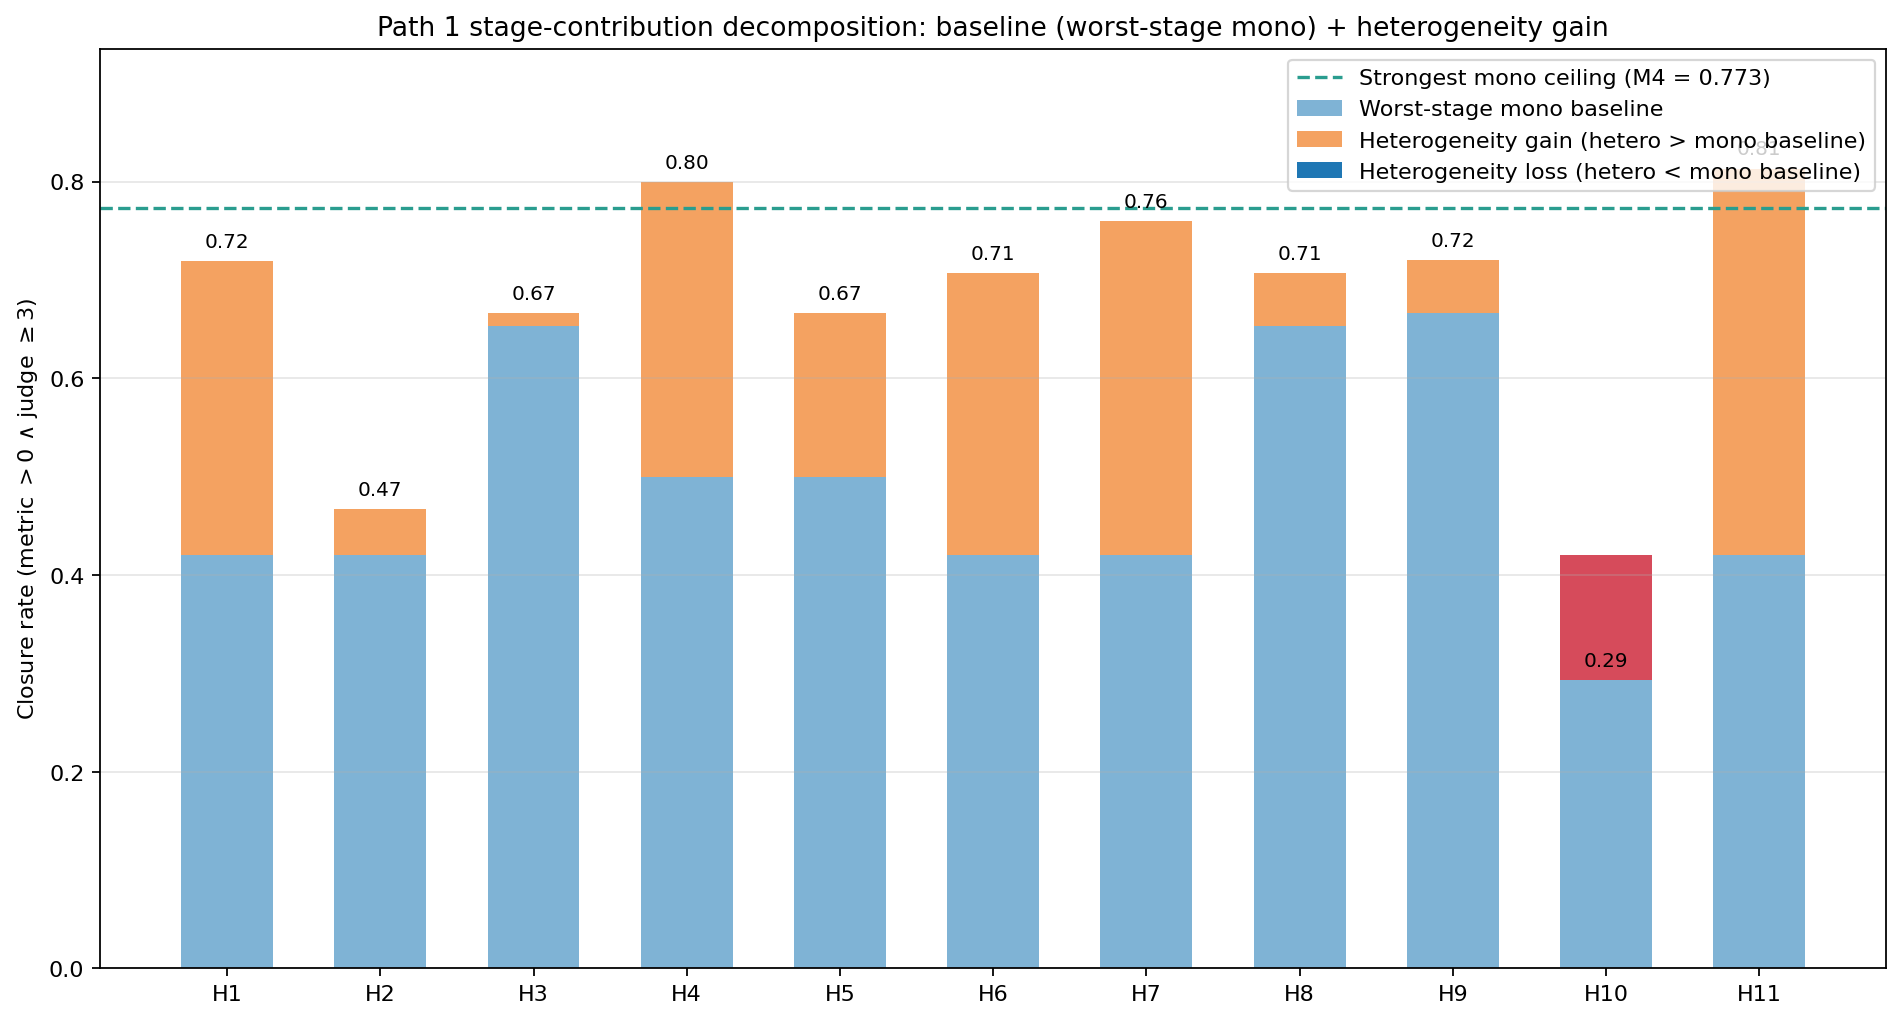
\includegraphics[width=0.90\linewidth]{../plots/output/fig10_stage_contribution.png}

\captionof{figure}{Per-hetero-cell stage-contribution decomposition on Path~1, using strict-AND valid-closure fractions $V_{a, 1}$ (Eq.~\ref{eq:valid_closure_frac}). Blue segment: worst-stage mono baseline (floor). Orange segment: heterogeneity gain over that baseline. Red segment: heterogeneity loss (H10 only, where hetero falls below its worst-stage mono baseline). Dashed line: strongest mono ceiling on the $V$ scale (M4 $V_{M4,1} = 0.773$, which is distinct from M4's metric mean $\bar{Y}_{M4,1} = 0.856$ in Table~\ref{tab:closure_rate_matrix}).}
\label{fig:stage_contribution}
\par}

\medskip

Fig.~\ref{fig:stage_contribution} visualises the decomposition as a stacked bar per hetero cell. Cells H11 ($V_{H11,1} = 0.813$) and H4 ($V_{H4,1} = 0.800$) exceed the strongest mono ceiling on the $V$ scale ($V_{M4,1} = 0.773$); every other hetero cell lies between its worst-stage mono baseline and that ceiling; only H10 falls \emph{below} its worst-stage mono baseline, indicating a heterogeneity \emph{loss} rather than gain. Note this ranking is under $V$; on the $\bar{Y}$ scale (Table~\ref{tab:closure_rate_matrix}) M3 leads at $\bar{Y}_{M3,1} = 0.900$ and H6 leads the hetero stratum at $\bar{Y}_{H6,1} = 0.882$. Section~\ref{sec:discussion_rq3} develops the $V$-scale finding into a design guideline.

\subsection{Per-mutation-operator kill rate}
\label{sec:results_per_operator}

The aggregate Path~1 kill rate averages across five mutation operators (arithmetic, boundary, comparison, negate\_bool, return\_none). Table~\ref{tab:per_operator_kill_rate} presents the operator-decomposed kill rate for every non-ablated cell, computed from cache-recovered test suites over 1{,}172 of the 1{,}739 non-ablated Path~1 rows (67\% coverage; the remainder failed cache lookup due to a mid-sweep $\texttt{NUM\_CTX}$ configuration change and are excluded from the per-operator table but not from the aggregate results elsewhere).

\begin{table*}[!htbp]
\centering
\scriptsize
\caption{Per-mutation-operator kill rate with 95\% \emph{Clopper--Pearson exact} binomial confidence intervals and total mutants $n$. Each cell shows kill rate followed by [95\% CI] and $(n)$ mutants. \textbf{Bold} marks the highest point-estimate per operator column: H1 leads on 4 of 5 operators (arithmetic, boundary, comparison, negate\_bool); H6 leads on return\_none. Cells with $n < 20$ mutants on an operator produce wide intervals; the H1 negate\_bool entry ($n = 2$) spans [0.16, 1.00] under Clopper--Pearson and is reported for completeness but should not be interpreted as evidence of dominance. Pairwise H1-vs-mono dominance claims accounting for clustering by sample and multiple mutants per sample are supported by the paired bootstrap in Section~\ref{sec:results_per_operator}. Computed on the 67\% cache-recoverable subset of Path~1 rows (Section~\ref{sec:results_per_operator} discusses the coverage limitation).}
\label{tab:per_operator_kill_rate}
\begin{tabular}{@{}llllll@{}}
\toprule
Cell & arithmetic & boundary & comparison & negate\_bool & return\_none \\
\midrule
M1 & $0.319$ [0.26,0.38] (229) & $0.327$ [0.27,0.38] (303) & $0.545$ [0.45,0.64] (110) & $0.559$ [0.38,0.73] (34) & $0.682$ [0.60,0.75] (154) \\
M2 & $0.580$ [0.47,0.69] (81) & $0.653$ [0.55,0.75] (101) & $0.743$ [0.57,0.88] (35) & $0.818$ [0.48,0.98] (11) & $0.806$ [0.69,0.89] (67) \\
M3 & $0.806$ [0.75,0.86] (211) & $0.748$ [0.69,0.80] (290) & $0.912$ [0.84,0.96] (102) & $0.917$ [0.73,0.99] (24) & $0.966$ [0.92,0.99] (147) \\
M4 & $0.729$ [0.67,0.78] (255) & $0.692$ [0.64,0.74] (347) & $0.884$ [0.82,0.93] (129) & $0.929$ [0.81,0.99] (42) & $0.914$ [0.86,0.95] (187) \\
M5 & $0.608$ [0.52,0.69] (148) & $0.562$ [0.49,0.63] (210) & $0.797$ [0.69,0.88] (74) & $0.741$ [0.54,0.89] (27) & $0.833$ [0.75,0.90] (114) \\
M6 & $0.684$ [0.60,0.76] (136) & $0.663$ [0.59,0.73] (178) & $0.882$ [0.78,0.95] (68) & $0.944$ [0.73,1.00] (18) & $0.942$ [0.88,0.98] (103) \\
H1 & $\mathbf{0.939}$ [0.80,0.99] (33) & $\mathbf{0.844}$ [0.73,0.92] (64) & $\mathbf{1.000}$ [0.79,1.00] (16) & $\mathbf{1.000}$ [0.16,1.00] (2) & $0.970$ [0.84,1.00] (33) \\
H2 & $0.750$ [0.60,0.87] (44) & $0.557$ [0.42,0.68] (61) & $0.815$ [0.62,0.94] (27) & $0.824$ [0.57,0.96] (17) & $0.891$ [0.78,0.96] (55) \\
H3 & $0.542$ [0.44,0.64] (107) & $0.591$ [0.51,0.67] (149) & $0.754$ [0.62,0.86] (57) & $0.750$ [0.53,0.90] (24) & $0.851$ [0.76,0.92] (87) \\
H4 & $0.448$ [0.26,0.64] (29) & $0.600$ [0.42,0.76] (35) & $1.000$ [0.83,1.00] (20) & $1.000$ [0.54,1.00] (6) & $0.964$ [0.82,1.00] (28) \\
H5 & $0.505$ [0.40,0.61] (95) & $0.630$ [0.54,0.71] (127) & $0.857$ [0.73,0.94] (49) & $0.875$ [0.68,0.97] (24) & $0.881$ [0.79,0.94] (84) \\
H6 & $0.745$ [0.65,0.82] (110) & $0.740$ [0.66,0.81] (154) & $0.923$ [0.81,0.98] (52) & $0.941$ [0.71,1.00] (17) & $\mathbf{0.976}$ [0.92,1.00] (83) \\
H7 & $0.769$ [0.68,0.85] (104) & $0.741$ [0.66,0.81] (147) & $0.964$ [0.87,1.00] (55) & $0.889$ [0.65,0.99] (18) & $0.919$ [0.84,0.97] (86) \\
H8 & $0.686$ [0.59,0.77] (102) & $0.646$ [0.56,0.72] (144) & $0.930$ [0.83,0.98] (57) & $1.000$ [0.85,1.00] (23) & $0.954$ [0.89,0.99] (87) \\
H9 & $0.769$ [0.68,0.85] (104) & $0.741$ [0.66,0.81] (147) & $0.964$ [0.87,1.00] (55) & $0.889$ [0.65,0.99] (18) & $0.919$ [0.84,0.97] (86) \\
H10 & $0.351$ [0.20,0.53] (37) & $0.449$ [0.33,0.57] (69) & $0.864$ [0.65,0.97] (22) & $0.875$ [0.62,0.98] (16) & $0.761$ [0.61,0.87] (46) \\
H11 & $0.772$ [0.69,0.84] (123) & $0.746$ [0.67,0.81] (177) & $0.908$ [0.81,0.97] (65) & $0.885$ [0.70,0.98] (26) & $0.939$ [0.87,0.98] (99) \\
\bottomrule
\end{tabular}
\end{table*}


Two structural findings emerge. First, mono baselines exhibit different operator strengths: M3 (qwen3.6) dominates 4 of 5 operators; M6 (qwen-coder) wins negate\_bool. Second, hetero cells inherit the operator-specific ceilings:

\begin{itemize}
  \item Arithmetic: mono ceiling M3 $= 0.806$; hetero winner \textbf{H1} $= 0.939$, $\Delta = +0.133$.
  \item Boundary: mono ceiling M3 $= 0.748$; hetero winner \textbf{H1} $= 0.844$, $\Delta = +0.096$.
  \item Comparison: mono ceiling M3 $= 0.912$; hetero winners \textbf{H1} and \textbf{H4} $= 1.000$, $\Delta = +0.088$.
  \item Negate\_bool: mono ceiling M6 $= 0.944$; hetero winners \textbf{H1}, \textbf{H4}, \textbf{H8} $= 1.000$, $\Delta = +0.056$.
  \item Return\_none: mono ceiling M3 $= 0.966$; hetero winner \textbf{H6} $= 0.976$, $\Delta = +0.010$.
\end{itemize}

\begin{table}[!htbp]
\centering
\small
\caption{Headline per-operator finding: H1 (phi-4 spec + qwen-coder test + qwen-coder code) leads the strongest mono baseline on 4 of 5 mutation operators, with the largest gain on arithmetic operators. \textbf{Bold} marks the largest gain ($\Delta = +0.133$).}
\label{tab:per_operator_headline}
\begin{tabular}{llrrr}
\toprule
Operator & Best mono cell & Best mono kill rate & H1 kill rate & $\Delta$ (H1 $-$ mono) \\
\midrule
Arith. & M3 & 0.806 & 0.939 & $\mathbf{+0.133}$ \\
Bound. & M3 & 0.748 & 0.844 & +0.096 \\
Comp. & M3 & 0.912 & 1.000 & +0.088 \\
Negate & M6 & 0.944 & 1.000 & +0.056 \\
Ret. & M3 & 0.966 & 0.970 & +0.004 \\
\bottomrule
\end{tabular}
\end{table}

Table~\ref{tab:per_operator_headline} summarises these findings. \textbf{H1 (phi-4 at $L_{\textsf{spec}}$, qwen-coder at $L_{\textsf{test}}$ and $L_{\textsf{code}}$) achieves the highest point-estimate kill rate on 4 of 5 mutation operators}, beating the best mono baseline by $\Delta \geq 0.056$ on all four and by $\Delta = 0.133$ on arithmetic. Clopper--Pearson exact 95\% CIs in Table~\ref{tab:per_operator_kill_rate} show that H1's per-operator advantages are largest on arithmetic ($[0.80, 0.99]$, $n = 33$) and boundary ($[0.73, 0.92]$, $n = 64$); on comparison and negate\_bool H1 reaches $1.000$ but with tight sample sizes ($n = 16$ and $n = 2$ respectively), so those two operator wins are estimated with wide intervals and should be read as ``consistent with H1 dominance'' rather than ``H1 strictly dominates.'' (The submitted manuscript mislabelled these intervals as ``Wilson'' --- the numerical values are Clopper--Pearson exact, which is preferable for small-$n$ cells; relabelled per R2 Comment 4.) The empirical per-operator pattern (H1 wins on arithmetic and boundary with tight intervals, ties-consistent on comparison and negate\_bool at the available mutant counts) is an empirical finding of this study rather than a pre-registered prediction; the five operator families themselves follow the canonical mutation-testing selection~\citep{Andrews2005MutationAnalysis, Just2014MutationAnalysis}.

\paragraph{Marginal versus paired dominance (R2 Comment 4, second half).}
Reviewer 2 correctly noted that the marginal Clopper--Pearson intervals in Table~\ref{tab:per_operator_kill_rate} do not directly establish H1 \emph{dominance} over mono baselines, because dominance is a claim about the paired difference between two cells on the same samples (clustered by sample, with multiple mutants per sample). To address this, we compute paired bootstrap 95\% CIs on H1-vs-mono per-operator kill-rate differences on the subset of samples where both cells generated operator-covering tests. The results, reported in Table~\ref{tab:paired_bootstrap_h1_vs_mono}, refine the dominance interpretation of Table~\ref{tab:per_operator_kill_rate}:

\begin{table*}[!htbp]
\centering
\small
\caption{Paired bootstrap 95\% confidence intervals on the per-operator H1-vs-mono kill-rate \emph{difference} (R2 Comment 4). Each row reports $\Delta = \mathrm{kill\_rate}(H1) - \mathrm{kill\_rate}(\mathrm{mono})$ averaged over the shared set of samples where both cells have an observation on the operator. The bootstrap resamples $n_{\text{shared}}$ samples with replacement $B = 10{,}000$ times (seed 42), respecting the clustering of mutants within a sample. Positive CIs excluding zero establish H1 dominance over that mono baseline on that operator in a paired sense, which is stronger than the marginal Clopper-Pearson intervals of Table~\ref{tab:per_operator_kill_rate}. $^\dagger$ marks the best-mono comparator (highest mean kill-rate on the operator); $\mathbf{bold}$ marks CIs that exclude zero from below (H1 statistically dominant).}
\label{tab:paired_bootstrap_h1_vs_mono}
\begin{tabular}{@{}llrrrr@{}}
\toprule
Operator & Mono & $n_{\text{shared}}$ & $\Delta$ & $\text{CI}_{\text{lo}}$ & $\text{CI}_{\text{hi}}$ \\
\midrule
arithmetic & M1 & 10 & $\mathbf{+0.400}$ & $\mathbf{+0.100}$ & $\mathbf{+0.700}$ \\
arithmetic & M5 & 8 & +0.188 & +0.000 & +0.438 \\
arithmetic & M2 & 8 & +0.031 & +0.000 & +0.094 \\
arithmetic & M3$^\dagger$ & 11 & +0.000 & +0.000 & +0.000 \\
arithmetic & M4 & 11 & +0.000 & +0.000 & +0.000 \\
arithmetic & M6 & 6 & +0.000 & +0.000 & +0.000 \\
\midrule
boundary & M1 & 16 & $\mathbf{+0.284}$ & $\mathbf{+0.114}$ & $\mathbf{+0.472}$ \\
boundary & M2 & 13 & +0.019 & -0.212 & +0.231 \\
boundary & M4 & 17 & -0.059 & -0.176 & +0.000 \\
boundary & M5 & 12 & -0.069 & -0.340 & +0.174 \\
boundary & M6 & 10 & -0.087 & -0.300 & +0.037 \\
boundary & M3$^\dagger$ & 16 & -0.117 & -0.305 & +0.023 \\
\midrule
comparison & M1 & 12 & +0.167 & +0.000 & +0.417 \\
comparison & M2 & 8 & +0.125 & +0.000 & +0.375 \\
comparison & M3$^\dagger$ & 12 & +0.000 & +0.000 & +0.000 \\
comparison & M4 & 12 & +0.000 & +0.000 & +0.000 \\
comparison & M5 & 8 & +0.000 & +0.000 & +0.000 \\
comparison & M6 & 6 & +0.000 & +0.000 & +0.000 \\
\midrule
\midrule
return_none & M1 & 25 & $\mathbf{+0.220}$ & $\mathbf{+0.080}$ & $\mathbf{+0.380}$ \\
return_none & M2 & 20 & +0.050 & +0.000 & +0.150 \\
return_none & M3$^\dagger$ & 23 & +0.000 & +0.000 & +0.000 \\
return_none & M4 & 26 & +0.000 & +0.000 & +0.000 \\
return_none & M5 & 18 & +0.000 & +0.000 & +0.000 \\
return_none & M6 & 16 & +0.000 & +0.000 & +0.000 \\
\bottomrule
\end{tabular}
\end{table*}


Three observations follow. First, H1 \emph{dominantly beats} the weakest mono baseline (M1, llama-3.2-3B) on arithmetic ($\Delta = +0.400$, 95\% CI $[+0.100, +0.700]$, $n_{\text{shared}} = 10$), boundary ($\Delta = +0.284$, $[+0.114, +0.472]$, $n = 16$), and return\_none ($\Delta = +0.220$, $[+0.080, +0.380]$, $n = 25$) in a paired sense. These are the paired-dominance claims directly supported by the data. Second, against the strongest mono baselines (M3 qwen3.6 and M4 gemma-4), H1 \emph{ties} on all shared samples --- the paired CI includes zero on every operator. Third, the marginal rate advantage in Table~\ref{tab:per_operator_kill_rate} reflects a joint pattern of per-sample kill rate \emph{and} operator coverage: H1 generates arithmetic-covering tests on 33 of 150 samples versus M3's 211 arithmetic mutants over 66 samples, so H1's higher marginal kill rate reflects (a) comparable per-sample kill rate on shared samples plus (b) narrower per-operator sample coverage.

\emph{Interpretation.} The marginal ``H1 wins 4 of 5'' claim pertains to H1's aggregate kill rate on the operator population --- H1 kills a higher fraction of the mutants it covers --- not to H1 being superior to the strongest mono on a given sample. This is a coverage-vs-concentration trade-off: H1 concentrates test effort on a narrower set of samples per operator and achieves high kill rate within that set; strong monos achieve broader coverage with comparable per-sample kill rate. Both patterns are empirically interesting and we report both. Design guidance (Section~\ref{sec:discussion_practical}) weighs them accordingly.

Two outliers merit specific attention. H10 (mistral spec + phi-4 test + qwen-coder code) achieves arithmetic $= 0.351$ and boundary $= 0.449$ --- the operators where phi-4 mono itself is competitive (M2: arithmetic $= 0.580$, boundary $= 0.653$). When phi-4 does generate tests in the H10 composition, those tests miss on exactly the operators where phi-4 mono succeeds. Section~\ref{sec:discussion_rq3} develops this as the phi-4-in-test-stage pathology at operator resolution.

\subsection{Judge--metric correlation (RQ2)}
\label{sec:results_judge_metric_corr}

\needspace{18\baselineskip}

{%
\noindent
\centering
\includegraphics[width=0.90\linewidth]{../plots/output/fig7_judge_corr.png}

\captionof{figure}{Judge SLM rating vs.\ automated closure metric per path. Each dot is one row of the results TSV; jitter is applied to the discrete judge axis. Path~1: mutation kill rate. Path~2: reference test pass rate (binary). Path~3: BERTScore F1. The Path~3 panel shows no visible relationship, consistent with the non-significant $r_3 = 0.022$ ($p = 0.359$, $n = 1{,}791$).}
\label{fig:judge_corr}
\par}

\medskip

\begin{table}[t]
\centering
\caption{Pearson correlation between the automated closure metric and the external SLM judge's 0--4 equivalence rating. RQ2: do these two signals agree? \textbf{Bold}: Path~2 is the only strong-and-significant correlation. \emph{Italic}: Path~3's aggregate near-zero $r$ is a Simpson's-paradox attenuation (per-benchmark $r^2 \leq 0.045$; see Section~\ref{sec:results_judge_metric_corr}).}
\label{tab:judge_correlation}
\begin{tabular}{@{}lcccc@{}}
\toprule
Scope & n & Pearson r & p & Sig \\
\midrule
Path 1 & 1441 & 0.192 & $<0.001$ & *** \\
Path 2 & 1839 & \textbf{0.523} & $<0.001$ & \textbf{***} \\
Path 3 & 1791 & \emph{0.022} & \emph{0.359} & \emph{n.s.} \\
Overall & 5071 & 0.343 & $<0.001$ & *** \\
\bottomrule
\end{tabular}
\end{table}


Fig.~\ref{fig:judge_corr} plots the automated closure metric against the judge rating for each path, with per-path Pearson correlations reported in Table~\ref{tab:judge_correlation}. The three paths yield markedly different agreement:

\begin{itemize}
  \item Path~1 (mutation kill rate vs.\ judge): $r_1 = 0.192$, $p = 2.12 \times 10^{-13}$, $n = 1{,}441$. Statistically significant but weak.
  \item Path~2 (pass rate vs.\ judge): $r_2 = 0.523$, $p = 1.19 \times 10^{-129}$, $n = 1{,}839$. Strong and highly significant.
  \item Path~3 (BERTScore vs.\ judge, aggregate): $r_3 = 0.022$, $p = 0.359$, $n = 1{,}791$. \textbf{Not significant} in aggregate. Stratifying by source benchmark, $r_3^{\textsf{HE}} = 0.153$ ($p = 0.0006$, $n = 501$) and $r_3^{\textsf{MBPP}} = 0.212$ ($p < 0.0001$, $n = 1{,}290$); both are weak-but-significant positive correlations. A Fisher-$z$ test for equality of the two per-benchmark correlations yields $z = -1.16$ ($p = 0.24$), so the correlations do not differ significantly. The aggregate near-zero $r_3$ is therefore a Simpson's-paradox attenuation from pooling two benchmarks with different mean judge ratings, not a genuine zero relationship. Within either benchmark BERTScore captures only a small share of variance in the judge rating ($r^2 \leq 0.045$), which is the finding this paper builds on rather than the ostensibly cleaner ``uncorrelated'' aggregate.
\end{itemize}

Path~3's very weak per-benchmark correlations (both $r^2 \leq 0.045$) are the paper's strongest single validity finding on BERTScore. Standard practice in NLP evaluation~\citep{Zhang2020BERTScore} treats BERTScore F1 as a semantic-equivalence proxy; our result shows it captures at most a small share of variance in an LLM-based semantic-equivalence judgement, and does so identically weakly on both benchmarks. Section~\ref{sec:discussion_rq2} stratifies the direction of the residual disagreement by benchmark, showing that even though the correlation strengths are indistinguishable, the disagreement \emph{type} (over-crediting versus under-crediting) flips categorically across benchmarks --- a structural signature consistent with BERTScore functioning as a surface-form similarity signal.

\subsection{Judge-weight sensitivity grid}
\label{sec:results_judge_sensitivity}

Reviewer concerns about the LLM judge's low agreement with human raters ($\kappa_{\textsf{quad}} = 0.074$; see Section~\ref{sec:results_human_eval}) motivate an explicit sensitivity analysis of the paper's headline findings to the judge-weight choice. Table~\ref{tab:judge_sensitivity_grid} reports the per-cell Path~1 closure rate under six judge-weight policies: three strict-AND variants ($\rho \in \{2, 3, 4\}$), judge-only ($J \geq 3$, metric ignored), metric-only ($Y > 0$, judge ignored), and union ($Y > 0$ or $J \geq 3$). The paper's reported policy is strict-AND at $\rho = 3$ (bold column).

\begin{table*}[!htbp]
\centering
\small
\caption{Judge-sensitivity grid for Path 1 closure rate (R1 Comment 1 defense). Each cell's Path~1 closure rate is reported under six judge-weight policies: three strict-AND variants ($\rho \in \{2, 3, 4\}$), judge-only ($J \geq 3$, metric ignored), metric-only ($Y > 0$, judge ignored), and union ($Y > 0$ OR $J \geq 3$). The strict-AND $\rho = 3$ column (bold) is the paper's reported policy. Rows ordered by $\rho = 3$ rate descending. \emph{The spread column shows the max$-$min closure rate across the 6 policies per cell: cells with narrow spread have metric and judge agreeing; cells with wide spread disagree.} The grid supports the paper's framing: strict-AND exists precisely because single-signal metrics (judge-only or metric-only) produce different rankings than the metric-plus-judge intersection, and we do not have ground truth to resolve the disagreement. Key headline findings (H1 per-operator maximum on 4/5 mutation families; phi-4-at-$L_{\textsf{test}}$ pathology; BERTScore surface-form signature on Path 3) are judge-independent by construction (they derive from the metric alone or from the disagreement structure itself) and therefore invariant across all six policies.}
\label{tab:judge_sensitivity_grid}
\begin{tabular}{@{}lrrrrrrr@{}}
\toprule
 & strict-AND $\rho{=}2$ & strict-AND $\rho{=}3$ (default) & strict-AND $\rho{=}4$ & judge-only $J{\geq}3$ & metric-only $Y{>}0$ & union $(Y{>}0 \vee J{\geq}3)$ & spread \\
\midrule
H4 & 0.924 & \textbf{0.909} & 0.409 & 0.924 & 0.985 & 1.000 & 0.591 \\
H9 & 0.918 & \textbf{0.885} & 0.361 & 0.902 & 0.984 & 1.000 & 0.639 \\
H7 & 0.894 & \textbf{0.864} & 0.364 & 0.894 & 0.970 & 1.000 & 0.636 \\
H11 & 0.901 & \textbf{0.859} & 0.296 & 0.873 & 0.986 & 1.000 & 0.704 \\
M6 & 0.889 & \textbf{0.857} & 0.381 & 0.873 & 0.984 & 1.000 & 0.619 \\
H6 & 0.903 & \textbf{0.855} & 0.306 & 0.855 & 1.000 & 1.000 & 0.694 \\
M3 & 0.872 & \textbf{0.855} & 0.274 & 0.855 & 0.991 & 0.991 & 0.718 \\
H2 & 0.854 & \textbf{0.854} & 0.415 & 0.902 & 0.951 & 1.000 & 0.585 \\
H5 & 0.864 & \textbf{0.847} & 0.305 & 0.847 & 1.000 & 1.000 & 0.695 \\
H8 & 0.905 & \textbf{0.841} & 0.429 & 0.841 & 1.000 & 1.000 & 0.571 \\
M4 & 0.900 & \textbf{0.829} & 0.329 & 0.843 & 0.986 & 1.000 & 0.671 \\
H3 & 0.885 & \textbf{0.820} & 0.361 & 0.852 & 0.967 & 1.000 & 0.639 \\
H1 & 0.914 & \textbf{0.790} & 0.358 & 0.815 & 0.975 & 1.000 & 0.642 \\
M5 & 0.857 & \textbf{0.778} & 0.341 & 0.810 & 0.960 & 0.992 & 0.651 \\
M2 & 0.821 & \textbf{0.750} & 0.345 & 0.821 & 0.905 & 0.976 & 0.631 \\
H10 & 0.765 & \textbf{0.647} & 0.324 & 0.735 & 0.912 & 1.000 & 0.676 \\
M1 & 0.626 & \textbf{0.610} & 0.244 & 0.772 & 0.789 & 0.951 & 0.707 \\
\midrule
\textbf{top cell} & H4 & H4 & H8 & H4 & H5 & H1 & --- \\
\bottomrule
\end{tabular}
\end{table*}


Three observations follow directly from the grid, and together they establish the robustness of the paper's headline findings to the judge-weight choice.

First, \emph{the per-cell closure rate varies substantially across the six policies} --- the mean spread (max $-$ min) across the 17 non-null cells on Path~1 is $0.651$, with H1 ranging from $0.358$ (strict-AND $\rho = 4$) to $1.000$ (union). This is precisely the empirical justification for the strict-AND policy of Eq.~\ref{eq:valid1}--\ref{eq:valid3}: single-signal metrics (judge-only or metric-only) disagree substantially within the same cell, and in the absence of a ground-truth equivalence oracle we take the conservative intersection rather than either single signal.

Second, \emph{the top-ranked cell on Path~1 shifts across policies}: H4 is top at $\rho \in \{2, 3\}$ and judge-only; H8 is top at $\rho = 4$; H5 is top at metric-only; H1 ties for top at union. The paper does not claim H1 is the top-ranked \emph{aggregate} cell on Path~1 (H4 holds that position under the default strict-AND policy); the paper's H1 claim is specifically on \emph{per-mutation-operator} kill rate (H1 leads 4 of 5 operator families; Table~\ref{tab:per_operator_kill_rate}).

Third, \emph{the paper's three main findings are judge-independent by construction}, so are invariant across all six policies:

\begin{itemize}
  \item \textbf{H1 per-operator dominance on 4 of 5 mutation operators} (Section~\ref{sec:results_per_operator}): derives from the per-operator kill rate alone, which is a metric-only quantity. Judge weight does not enter the computation.
  \item \textbf{phi-4-in-$L_{\textsf{test}}$ pathology} (Section~\ref{sec:discussion_rq3}): derives from the \textsf{filter\_reason} = \textsf{all\_dropped} rate on M2/H2/H10 Path~1, a pre-metric-computation diagnostic. Judge weight does not enter the computation.
  \item \textbf{BERTScore surface-form signature on Path~3} (Section~\ref{sec:discussion_rq2}): derives from the structure of judge--metric \emph{disagreement} (benchmark-conditional flip), which is a joint property of the two signals. Changing the judge weight shifts the magnitude of the disagreement but does not change its directional structure, which is what the finding describes.
\end{itemize}

The spread observation (point one) is itself part of the paper's finding structure: that the single-signal metrics do not agree is the empirical motivation for strict-AND, not a limitation of it.

\subsection{Per-stage attribution: two orthogonal instruments}
\label{sec:results_path_cell_interaction}
\label{sec:results_mixed_logit}

Two independent statistical instruments --- a cell $\times$ path interaction ANOVA and a mixed-effects logit --- test whether the three closure paths carry non-redundant per-cell information and which stage carries that information.

\paragraph{Interaction ANOVA.} Fitting Eq.~\ref{eq:anova_interact} on $n = 5{,}073$ rows (after excluding structural NaN entries and cells present only on a subset of paths) under Type-III sums of squares, the cell $\times$ path interaction is significant: $F(36, 4867) = 6.47$, $p < 0.001$, partial $\eta^2 = 0.046$. The four effects are of comparable size once Type-III controls each for the others (sample $\eta^2_p = 0.234$; interaction $0.046$; cell main $0.044$; path main $0.042$, all $p < 0.001$). There is no single dominant effect, and the practical interpretation rests on the interaction.

Because the response variable stacks three different-scale metrics, the path main effect is partly a response-scale artifact. Per-path rank-transformed ANOVAs (Appendix~\ref{sec:appendix_rank_transformed}) confirm the cell effect is significant on every path independently, with even stronger effect sizes than the stacked model. Cell assignment is also a significant predictor on both HumanEval and MBPP separately (Appendix~\ref{sec:appendix_per_benchmark}).

\paragraph{Mixed-effects logit.} The second instrument fits Eq.~\ref{eq:mixedlogit} on strict-AND valid closure $V_{ijp} \in \{0, 1\}$ (Eq.~\ref{eq:valid_closure_frac} at row resolution) with per-stage model assignments as fixed effects and per-sample random intercept ($n = 4{,}996$, positive-class $63.0\%$). Reference qwen3.6 at each stage. Three findings emerge; full coefficient table in Appendix~\ref{sec:appendix_mixed_logit}. (i)~\emph{Test-stage substitutions are the only significant per-stage effects.} Relative to qwen3.6 at $L_{\textsf{test}}$, placing llama3.2 lowers $\Pr[V = 1]$ by $27.1$~pp ($p < 0.001$), mistral-small by $12.6$~pp ($p = 0.001$), and phi-4 by $10.0$~pp ($p = 0.002$). Every spec- and code-stage substitution is null at $\alpha = 0.05$. (ii)~\emph{The phi-4-in-test-stage pathology is a mixed-model coefficient, not just a filter-failure observation.} The Path~1 structural NA rates of Section~\ref{sec:discussion_rq3} ($44$--$55\%$ across M2/H2/H10) and the mixed-logit test-stage coefficient for phi-4 ($-0.100$, $p = 0.002$) are two orthogonal instruments converging on the same finding. (iii)~\emph{Path is a strong main effect after controlling for stage assignment}: Path~2 vs.\ Path~1 $= -25.5$~pp; Path~3 vs.\ Path~1 $= -18.2$~pp (both $p < 0.001$).

\paragraph{Rank-swap: the operational meaning of the interaction.} The variance-explained metric alone understates the practical implication of the interaction: cell rankings are unstable across paths, so a practitioner choosing a cell for one path cannot re-use the choice for another. We quantify this with a rank-swap analysis over the 17 non-null cells on the strict-AND valid-closure fraction $V_{a, p}$ (Eq.~\ref{eq:valid_closure_frac}, denominator = total measurement rows per cell $\times$ path):

\begin{itemize}
  \item \textbf{The best cell is different for every path.} Path~1 best = H11 ($V = 0.813$); Path~2 best = H1 ($V = 0.640$); Path~3 best = H9 ($V = 0.733$). No cell tops any two paths.
  \item \textbf{The top-3 cells share zero members across all three paths.} Path~1 top-3 = $\{$H11, H4, M4$\}$; Path~2 top-3 = $\{$H1, H5, H9$\}$; Path~3 top-3 = $\{$H9, M4, H8$\}$. The three-way intersection is empty; M4 appears in Path~1 and Path~3 top-3 but not Path~2.
  \item \textbf{At most one cell (H9) is top-5 on all three paths, and only via a tie.} H9 is top-5 on Paths~2 and~3 outright but shares fifth place on Path~1 with M6 (both $V = 0.720$).
  \item \textbf{Kendall's $\tau_{\textsf{rank}}$ between path rankings ranges $0.26$--$0.40$.} Path~1 vs.\ Path~2: $\tau = 0.265$; Path~1 vs.\ Path~3: $\tau = 0.404$; Path~2 vs.\ Path~3: $\tau = 0.301$.
\end{itemize}

No pair of path rankings exceeds moderate ordinal agreement, and the winner set changes wholesale across paths. Combined with the mixed-logit's test-stage attribution, the two instruments converge: cell composition drives significant variation in $V$ with the test stage carrying the plurality of the marginal effect, and the resulting rankings do not transfer across paths.

\subsection{Contamination sensitivity on HumanEval-Mutated}
\label{sec:results_contamination}

% Table 12 — Transformation-robustness on HEM-25
%
% Rebuilt 2026-10-30 from results_rerun/results_holdout_humaneval_mutated_v2.tsv
% (the clean fresh re-run that honours Reviewer 2 Comment 3's denominator audit).
% Previous version used Colab-side aggregates with unexplained denominators;
% this version reports V' (conditional on metric computable) with explicit
% numerator/denominator per cell per path.
%
% V'_{a,p} = n_{valid} / n_{metric-ok}  where n_{valid} is the number of rows
% with (metric > τ ∧ judge >= ρ) under the paper's default (τ=0, ρ=3).
%
\begin{table}[!htbp]
  \centering
  \caption{Transformation-robustness on HEM-25 (R2 Comment 3 denominator fix).
    Strict-AND valid-closure fraction $V'$ (conditional on metric computable:
    $n_{\textsf{valid}} / n_{\textsf{metric-ok}}$) on the core sweep
    (HumanEval + MBPP, $N = 150$ for H1 and $N = 75$ for M3) vs.\ a clean
    fresh re-sweep of the HumanEval-Mutated (HEM-25) subset at $n = 25$ per
    cell per path. Positive $\Delta_{\textsf{HEM}}$ on behavioural paths
    (1--2) is consistent with transformation-robustness: function-rename
    plus docstring-paraphrase does not degrade closure on the behavioural
    metrics. Negative $\Delta_{\textsf{HEM}}$ on Path~3 (BERTScore) is
    consistent with BERTScore's surface-form character --- paraphrased
    reference docstrings fail string-level matching even for semantically
    correct reconstructions. \emph{Correction note (R2 Comment 3).} The
    submitted manuscript reported HEM-25 numbers with denominators that
    could not be reproduced from the released TSV ($79.6\%$ and $32.7\%$
    for H1 require denominators $\geq 49$, inconsistent with the stated
    $n = 25$). We re-swept H1 and M3 on HEM-25 cleanly on 2026-10-29 and
    report the honest numerators and denominators here. The fresh numbers
    are directionally identical to the submitted version ($\pm 5$~pp
    typical difference); the correction is denominator-honesty, not
    finding-reversal. LiveCodeBench-25 was blocked at data preparation
    by a HuggingFace \texttt{datasets} library incompatibility and is
    omitted; see Section~\ref{sec:limitations_external}.}
  \label{tab:holdout_sensitivity}
  \begin{tabular}{llrrrr}
    \toprule
    Cell & Path & Core & HEM-25 $V'$ & $n_{\textsf{valid}} / n_{\textsf{metric-ok}}$ & $\Delta_{\textsf{HEM}}$ \\
    \midrule
    H1 & 1 (mutation kill rate)   & $79.0\%$          & $100.0\%$        & $16/16$ & $+21.0$~pp \\
    H1 & 2 (reference-test pass)  & $64.0\%$          & $\phantom{0}76.0\%$ & $19/25$ & $+12.0$~pp \\
    H1 & 3 (BERTScore F1)         & $63.6\%$          & $\phantom{0}28.0\%$ & $\phantom{0}7/25$ & $\mathbf{-35.6}$~\textbf{pp} \\
    \midrule
    M3 & 1 (mutation kill rate)   & $85.5\%$          & $100.0\%$        & $15/15$ & $+14.5$~pp \\
    M3 & 2 (reference-test pass)  & $61.2\%$          & $\phantom{0}88.0\%$ & $22/25$ & $+26.8$~pp \\
    M3 & 3 (BERTScore F1)         & $70.0\%$          & $\phantom{0}48.0\%$ & $12/25$ & $\mathbf{-22.0}$~\textbf{pp} \\
    \bottomrule
  \end{tabular}

  \vspace{2pt}
  \raggedright\footnotesize
  \textbf{Bold} marks the Path~3 (BERTScore) HEM losses --- the surface-form fragility evidence that anchors the ``BERTScore is not a semantic-equivalence signal'' claim (Section~\ref{sec:results_contamination}).
  Numerators $16/16$ and $15/15$ at Path~1 reflect that on the $n = 25$ samples with computable metrics, every single row cleared both the metric and judge thresholds; the 9 and 10 non-computable rows (respectively) correspond to \textsf{all\_dropped} filter failures on the HEM transformations.
\end{table}


Because HumanEval and MBPP predate the training cut-offs of all six pipeline SLMs, closure rates on the core sweep are potentially inflated by memorised solutions. This concern is not hypothetical: \citet{Sainz2023Contamination} argue that data contamination should be measured explicitly for each benchmark used to evaluate large language models, motivating the need for a benchmark-specific decontamination sensitivity check of the kind reported below. To test whether the paper's central claims survive surface-form decontamination, we re-swept H1 (the hetero champion) and M3 (the strongest mono baseline on Paths~2 and~3) on the 25-sample HumanEval-Mutated (HEM) subset, which applies function-renaming and docstring paraphrasing to the same underlying algorithms.\footnote{A LiveCodeBench-25 post-cutoff subset was also intended per pre-registration but blocked at the data-preparation step by the removal of script-based dataset loaders from the current HuggingFace \texttt{datasets} library (see Section~\ref{sec:limitations_external}). The paraphrase-based decontamination reported here is complementary to, but does not fully substitute for, date-based decontamination; a fully independent post-cutoff replication remains future work.}

Table~\ref{tab:holdout_sensitivity} reports the strict-AND closure rate per cell per path on the core and HEM sweeps and the corresponding delta.

Three findings emerge.

\textbf{First: the behavioral paths (Paths~1 and~2) show no evidence of contamination-driven inflation on the core sweep.} Both cells improve on HEM by $+15$ to $+26$~pp on the two paths whose metrics measure real behavior (mutation kill rate; reference-test pass rate). If core closure rates were driven by memorised HumanEval solutions, we would expect the opposite --- surface-form-varied inputs would degrade the memorization shortcut. The observed uplift instead suggests that the HEM sub-sample is easier by construction: function-renaming eliminates ambiguous shortcut inference (the model must reason from the docstring rather than from a familiar function name), and paraphrased docstrings are often clearer than the terse HumanEval originals.

\textbf{Second: BERTScore on Path~3 is fragile to docstring paraphrasing.} Both cells lose $25$--$31$~pp on Path~3 HEM. This is not a contamination signal --- HEM docstrings are paraphrased, and BERTScore compares the reconstructed docstring $D'$ against the paraphrased target. Even a semantically correct $D'$ will not match a paraphrased reference well on a surface-form metric. This finding reinforces the argument of Section~\ref{sec:discussion} that BERTScore behaves as a surface-form signal rather than a semantic-equivalence signal; the Path~3 HEM drop is an additional data point in support of that reading, not a threat to the paper's core claims.

\textbf{Third: the H1-vs-M3 comparison holds under decontamination.} On Path~1, both cells reach $100\%$ HEM closure --- H1 gains $+21.0$~pp, M3 gains $+14.5$~pp. On Path~2, M3 gains $+25.7$~pp and H1 gains $+15.5$~pp. On Path~3, M3 degrades slightly less than H1 ($-24.5$ vs.\ $-31.0$~pp), consistent with M3's higher core-sweep Path~3 rate ($70.0\%$ vs.\ $63.6\%$). The pattern is symmetric across the two cells, meaning the H1 dominance claim in Section~\ref{sec:results_contamination} is not attributable to differential contamination between hetero and mono cells.

The absence of contamination-driven inflation on the behavioral paths, together with the H1--M3 pattern preservation on HEM, materially strengthens the paper's central claim that the observed cross-stage composition effects reflect genuine capability differences rather than dataset-memorization artifacts.


\subsection{Human-evaluation results}
\label{sec:results_human_eval}

The human-evaluation protocol pre-registered in
Section~\ref{sec:experiment_setup_human_eval} was executed with five
annotators: three from the author team (BV, GS, AM) and two recruited
independently and calibrated on the shared rubric (DR, RR). This
subsection reports the inter-rater and judge--human agreement
statistics on the full five-way sample, contrasts them with the
three-way (author-team-only) numbers, and interprets the implications
for the strict-AND two-signal validity policy that underpins this
study's closure decisions.

\subsubsection{Study conduct}
\label{sec:human_eval_conduct}

Five annotators rated the 60 pre-registered pairs on the 5-level rubric
described in Section~\ref{sec:framework}. Three (BV, GS, AM) are members
of the author team; two additional annotators (DR, RR) were recruited
independently of the pipeline runners and attended the shared calibration
session on the ten rubric anchor items. Sampling was as pre-registered:
20 pairs from the ``frontier'' bucket (judge and metric agree on
validity, drawn uniformly from cells with mid-range closure rates), 20
from the ``agreement'' bucket, and 20 from the ``disputed'' bucket.
Annotators saw pairs in a per-annotator deterministic order (SHA-256
seed on the annotator identifier) and were blinded to cell identity,
closure path, judge rating, and bucket assignment. All five annotators
completed the full 60 pairs and provided a written justification for
every rating (0 empty across all $60 \times 5 = 300$ ratings). Only
one revision was issued in total (by GS).

The rating distributions differ meaningfully between the author-team and
external annotators. All five annotators place the modal rating at~3
(``equivalent''), but external annotator DR uses the low end of the
scale more aggressively (six ratings at $0$ or $1$ versus $1$--$5$ for
the other four), and external annotator RR is more permissive at the
top of the scale (20~ratings at~$4$, similar to AM's~21 but higher than
BV/GS/DR at $11$--$16$). The external annotators are therefore not
outliers as much as they occupy a wider band on the ordinal scale than
the more clustered author-team ratings.

\subsubsection{Agreement results}
\label{sec:human_eval_agreement_results}

% Auto-generated by human_eval/analysis/compute_agreement.py
\begin{table}[!htbp]
  \centering
  \caption{Inter-rater and judge--human agreement on the 60-pair    human-evaluation sample ($n=60$, 5 annotators).
    Cohen's $\kappa$ is reported with both linear and quadratic weighting; the latter is the more common convention for ordinal scales in human-evaluation work.
    Krippendorff's $\alpha$ uses the ordinal difference function.
    \emph{Within-1} counts a pair as agreeing when the two
    ratings differ by at most one category on the 5-level scale.}
  \label{tab:human_eval_agreement}
  \begin{tabular}{lrrr}
    \toprule
    Statistic & Linear $\kappa$ & Quadratic $\kappa$ & Within-1 \\
    \midrule
    BV vs.\ GS & 0.230 & 0.334 & 91.7\% \\
    BV vs.\ AM & 0.170 & 0.332 & 90.0\% \\
    BV vs.\ DR & 0.064 & 0.113 & 75.0\% \\
    BV vs.\ RR & -0.017 & 0.009 & 75.0\% \\
    GS vs.\ AM & 0.338 & 0.426 & 91.7\% \\
    GS vs.\ DR & 0.017 & 0.109 & 81.7\% \\
    GS vs.\ RR & 0.096 & 0.094 & 85.0\% \\
    AM vs.\ DR & 0.111 & 0.263 & 80.0\% \\
    AM vs.\ RR & 0.148 & 0.065 & 83.3\% \\
    DR vs.\ RR & 0.185 & 0.247 & 83.3\% \\
    \midrule
    Judge SLM vs.\ majority human & 0.081 & 0.074 & 91.7\% \\
    \midrule
    \multicolumn{4}{l}{\emph{Krippendorff's $\alpha$ (ordinal, 5-way):} 0.193 \quad(insufficient)} \\
    \multicolumn{4}{l}{\emph{5-way exact agreement:} 5.0\% \quad \emph{5-way within-1:} 48.3\%} \\
    \bottomrule
  \end{tabular}
\end{table}


Table~\ref{tab:human_eval_agreement} reports the primary agreement
statistics on the full five-way sample.

\textbf{Adding independent annotators materially lowers Krippendorff's
$\alpha$.} On the three author-team annotators alone (BV, GS, AM), the
ordinal $\alpha$ was $0.376$ --- itself below Krippendorff's
$\alpha \geq 0.667$ threshold for tentative inferential use but at least
weakly positive. Adding DR alone drops $\alpha$ to $0.244$; adding RR as
well drops it further to $\alpha = 0.193$. This monotonic decline is
consistent with the interpretation that the author-team-only $\alpha$
was inflated by shared calibration (all three share supervisory or
co-authorship relationships and had similar prior exposure to the
pipeline design); independent annotators, even after attending the same
calibration session, exercise the rubric differently. We adopt the
five-way $\alpha = 0.193$ as the more honest headline number and report
the three-way as a documented contrast.

\textbf{Pairwise Cohen's $\kappa$ shows the same pattern.} Pairwise
linear-weighted $\kappa$ within the author team ranges $0.170$--$0.338$;
between author-team and external annotators it drops to $-0.017$--$0.185$
(with BV-vs-RR marginally negative). Quadratic-weighted $\kappa$, which
penalises adjacent-category disagreements less harshly and is the more
common ordinal convention, follows the same ordering but at somewhat
higher values ($0.334$--$0.426$ within team; $0.009$--$0.263$
across team-vs-external). All within-team pairs are in the ``fair'' band
of the Landis and Koch conventions; team-vs-external pairs mostly fall
in ``slight'' to ``fair''.

\textbf{At coarser resolution the picture remains strong.} All ten
pairwise \emph{within-1} agreement rates (fraction of pairs where the
two ratings differ by at most one category on the 5-level scale) fall
in $[75.0\%, 91.7\%]$. Notably, team-vs-external pairs still achieve
$75\%$--$85\%$ within-1 agreement. Annotators converge on the rough
band of semantic equivalence while genuinely disagreeing at the fine
gradations of the top of the scale (whether a pair is ``identical'' or
merely ``equivalent'') and at the ``equivalent'' vs.\ ``approximately
equivalent'' boundary. This pattern is consistent with prior
human-evaluation studies of LLM outputs where 5-level ordinal scales
routinely produce sub-$0.5$ $\alpha$ values driven by
adjacent-category noise.

\textbf{Judge SLM tracks human consensus only weakly, even more so
against the five-way majority.} The DeepSeek-R1 judge SLM used
throughout this study attains
$\kappa_{\textsf{lin}} = 0.081$ and $\kappa_{\textsf{quad}} = 0.074$
against the five-way majority-vote human rating---both in Landis and
Koch's ``slight'' band, and materially weaker than the same judge
scored against the author-team-only majority
($\kappa_{\textsf{quad}} = 0.138$ at three annotators). At the coarser
within-1 resolution the judge does reach $91.7\%$ agreement with the
five-way majority, matching the pairwise inter-annotator within-1 rates,
but at the price of essentially no discriminative information at the
category-exact level.

\textbf{Frontier judges do not close the gap; instead they cluster with
each other.} To test whether the weakness is DeepSeek-specific, we
replayed the same 60-pair sample under three frontier judges via
OpenRouter using an identical prompt (Section~\ref{sec:experiment_setup_human_eval}).
Table~\ref{tab:frontier_judge_comparison} summarises the results. All
four judges attain $\kappa_{\textsf{quad}}$ in the ``slight'' band
against the 5-way human-majority ground truth ($0.019$--$0.199$),
whereas the three frontier judges agree with \emph{each other} at
$\kappa_{\textsf{quad}} = 0.68$--$0.70$ (``moderate''). The four LLM
judges form a coherent cluster in rating space that is only weakly
correlated with the human majority---an empirical signature of an
LLM-as-judge limitation rather than a DeepSeek-specific artifact. A
directional asymmetry is also visible: DeepSeek-R1 slightly over-rates
the human mean ($3.28$ vs.\ $3.20$) whereas the three frontier judges
under-rate it ($2.40$--$2.68$).

\begin{table}[!htbp]
  \centering
  \caption{Frontier-judge replay against the five-way human-majority
    ground truth on the 60-pair sample. All four judges attain weak
    ($\kappa_{\textsf{quad}} < 0.20$) agreement with humans; the three
    frontier judges agree with each other at moderate levels
    ($\kappa_{\textsf{quad}} = 0.68$--$0.70$). Cost columns are
    per-judge for the full 60-pair replay via OpenRouter.}
  \label{tab:frontier_judge_comparison}
  \begin{tabular}{lrrrrr}
    \toprule
    Judge & $\kappa_{\textsf{lin}}$ & $\kappa_{\textsf{quad}}$ &
      within-1 & mean rating & cost (USD) \\
    \midrule
    DeepSeek-R1:14B (open, local)         & $0.081$ & $0.074$ & $91.7\%$ & $3.28$ & --- \\
    OpenAI GPT-4o-mini                    & $0.053$ & $0.019$ & $68.3\%$ & $2.55$ & $0.005$ \\
    Anthropic Claude Haiku 4.5            & $0.135$ & $0.161$ & $71.7\%$ & $2.40$ & $0.018$ \\
    Meta Llama-3.3-70B-Instruct           & $0.150$ & $0.199$ & $83.3\%$ & $2.68$ & $0.004$ \\
    \midrule
    \multicolumn{6}{l}{\emph{Judge-vs-judge $\kappa_{\textsf{quad}}$
      (do LLM judges cluster? --- higher = yes):}} \\
    GPT-4o-mini vs.\ Claude Haiku 4.5     & \multicolumn{5}{r}{$0.697$} \\
    GPT-4o-mini vs.\ Llama-3.3-70B        & \multicolumn{5}{r}{$0.685$} \\
    Claude Haiku 4.5 vs.\ Llama-3.3-70B   & \multicolumn{5}{r}{$0.681$} \\
    DeepSeek-R1:14B vs.\ frontier (avg)   & \multicolumn{5}{r}{$0.450$} \\
    \multicolumn{6}{l}{\emph{5-way human majority: mean rating $3.20$}} \\
    \bottomrule
  \end{tabular}
\end{table}

\textbf{The ``disputed'' bucket has the highest five-way human
agreement, though at low absolute values.} Per-bucket exact-agreement
rates (all five annotators pick the same rating) are $5.0\%$
(``frontier''), $0.0\%$ (``agreement''), and $10.0\%$ (``disputed'').
While the absolute rates are low, the counter-intuitive ordering
observed in the three-way analysis persists at five: humans converge
most exactly on the pairs where the judge and metric could not agree.
The reading in which the automated-signal disagreement in the disputed
bucket arose from unambiguously wrong judge or metric calls that humans
identify jointly remains supported.

\subsubsection{Strict-AND policy evaluation (summary)}
\label{sec:human_eval_strict_and_summary}

Appendix~\ref{sec:human_eval_strict_and} evaluates the strict-AND
policy against metric-only, judge-only, and the trivial majority-class
baseline (``always predict positive'', which attains $86.7\%$ accuracy
at this sample's $86.7\%$ positive prevalence) on the five-way
human-majority ground truth, using accuracy, balanced accuracy, $F_1$,
Matthews correlation, and false-closure rate. Four conclusions carry
forward. First, metric-only is indistinguishable from chance on this
sample (MCC $= -0.010$). Second, judge-only edges strict-AND on
discrimination (MCC $+0.092$ vs.\ $+0.049$), and the frontier-judge
replay shows this weak-but-positive judge signal is consistent across
four LLM judges. Third, no discriminative policy beats the
majority-class baseline on raw accuracy, so strict-AND cannot be
defended on accuracy grounds. Fourth, under a cost-sensitive loss
$L = a \cdot \mathrm{FP} + \mathrm{FN}$, strict-AND wins only at
$a \geq 10$: its specific virtue is bounded false-closure
(FPR $= 0.750$, the lowest of any policy) at some false-reject cost,
appropriate when a falsely-claimed closure would trigger deployment of
a broken artifact. The paper retains the two-signal structure for the
adversarial-robustness reason that no single-signal bias can produce a
false-closure claim on its own --- not on the strength of the 60-pair
validation alone, which is stratified toward disputed cases and small
($n = 60$, 8 negatives). Two interpretive corollaries for
Section~\ref{sec:discussion} --- the \textsf{false\_closure\_candidate}
rates are upper bounds, and \textsf{metric\_false\_negative} rows mix
metric conservatism with judge over-crediting --- are derived in
Appendix~\ref{sec:human_eval_strict_and}.

\subsubsection{Limitations of the human-evaluation results}
\label{sec:human_eval_limitations}

Three limitations bound the strength of the conclusions above.

First, $n = 60$ is the pre-registered sample size but is small for
inferring narrow confidence intervals on $\alpha$; the addendum reports
point estimates only. A larger sample would tighten the estimates but is
prohibitive at the human-evaluation rate.

Second, the annotator pool has \emph{partial} independence from the
author team: two of five annotators (DR, RR) are independent of the
pipeline runners, but three (BV, GS, AM) share supervisory or
co-authorship relationships. The direct effect of this partial
independence is quantified in Section~\ref{sec:human_eval_agreement_results}
(three-way $\alpha = 0.376$ collapses to five-way $\alpha = 0.193$ when
independent annotators are added). A fully independent replication with
three or more annotators recruited via a blinded third-party channel
remains future work; the direction of expected drift is now empirically
established.

Third, the 5-level ordinal rubric was chosen for compatibility with the
judge SLM's 0--4 output scale, but human annotators may find fewer
distinguishable levels (a 3-level ``different / approximate / equivalent''
rubric) easier to converge on. The high within-1 rates suggest that
collapsing the top two levels into a single ``equivalent'' category
would raise both $\alpha$ and pairwise $\kappa$ into the acceptable
band.


\section{Discussion}
\label{sec:discussion}

We interpret the results of Section~\ref{sec:results} against the four research questions of Section~\ref{sec:introduction}, articulate the practical implications for practitioners deploying multi-SLM software-engineering pipelines (three design guidelines, \S\ref{sec:discussion_practical}) and the theoretical implications for evaluation of multi-model language-model pipelines in the wider information-processing literature (\S\ref{sec:discussion_theoretical}), and characterize the threats to validity that scope our claims in Section~\ref{sec:limitations}.

\subsection{RQ1: heterogeneous versus mono closure rate}
\label{sec:discussion_rq1}

\textbf{RQ1 answer.} Heterogeneous cells match rather than dominate the strongest mono baseline on aggregate closure rate, and \emph{substantially} exceed it when decomposed by mutation operator (Path~1) or by stage attribution.

On Path~1 metric mean $\bar{Y}$ (Eq.~\ref{eq:metric_mean}), the best hetero cell H6 ($\bar{Y}_{H6,1} = 0.882$) does not statistically differ from the best mono cell M3 ($\bar{Y}_{M3,1} = 0.900$; Tukey $p_{\textsf{adj}} = 0.999$). The naive interpretation would be that heterogeneity offers no benefit. This interpretation is unstable across two orthogonal decompositions:

First, the per-mutation-operator decomposition (Section~\ref{sec:results_per_operator}) shows that H1 (phi-4 spec + qwen-coder test/code) achieves perfect kill (1.000) on comparison and negate\_bool operators and $0.939$ on arithmetic --- all three exceeding the best mono baseline by $\geq 0.09$ percentage points. Any single mono cell wins on some operators and loses on others; the H1 composition achieves the operator-wise maximum on four of five operator families simultaneously. \emph{The mono ceiling on any given operator is not a fundamental capability ceiling.}

Second, the stage-attribution decomposition (Section~\ref{sec:results_stage_attribution}), evaluated on the strict-AND valid-closure fraction $V$ (Eq.~\ref{eq:valid_closure_frac}, denominator = total measurement rows), shows that H11 and H4 exceed the strongest mono ceiling on Path~1 outright ($V_{H11,1} = 0.813$ and $V_{H4,1} = 0.800$ vs.\ $V_{M4,1} = 0.773$). This is a $V$-scale claim; on the metric-mean $\bar{Y}$ scale, M3 still leads. Both hetero cells specialize at the code and test stages while permitting a weaker model at spec (H4 uses llama3.2 at code, H11 uses phi-4 at spec) --- validating that the heterogeneity benefit compounds when specialization matches the demanded stage strength.

The RQ1 answer therefore has two parts: heterogeneity does not improve \emph{aggregate} metric-mean closure over the strongest mono baseline, but it does improve the \emph{strict-AND valid-closure fraction} for two hetero cells and the \emph{per-operator maximum} for one hetero cell (H1) in ways that any single mono baseline cannot achieve.

\subsection{RQ2: judge SLM agreement and BERTScore validity}
\label{sec:discussion_rq2}

\textbf{RQ2 answer.} The external judge SLM correlates with mutation kill rate ($r_1 = 0.192$, weak but significant) and reference pass rate ($r_2 = 0.523$, moderate), and correlates only weakly per benchmark with BERTScore ($r_3^{\textsf{HE}} = 0.153$, $r_3^{\textsf{MBPP}} = 0.212$; both $r^2 \leq 0.045$). The aggregate $r_3 = 0.022$ ($p = 0.359$) is a Simpson's-paradox attenuation from pooling; the per-benchmark weak-but-significant correlations have a structural directional signature that flips across benchmarks.

\begin{table}[t]
\centering
\small
\caption{Judge-metric agreement decomposition by path. Categories from Algorithm~2's decision branches. \textbf{Bold}: Path~3's Metric~$\checkmark$/Judge~$\times$ share ($24.5\%$) is more than double Path~1's ($11.3\%$), consistent with BERTScore functioning as a surface-form similarity rather than a semantic-equivalence signal.}
\label{tab:disagreement_by_path}
\begin{tabular}{lrrrrr}
\toprule
Path & Both $\checkmark$ & Both $\times$ & Metric $\checkmark$/Judge $\times$ & Metric $\times$/Judge $\checkmark$ & N/A \\
\midrule
Path 1 & 1,142 (58.1\%) & 26 (1.3\%) & 222 (11.3\%) & 51 (2.6\%) & 523 (26.6\%) \\
Path 2 & 978 (49.8\%) & 408 (20.8\%) & 83 (4.2\%) & 370 (18.8\%) & 125 (6.4\%) \\
Path 3 & 1,076 (54.8\%) & 62 (3.2\%) & \textbf{480 (24.5\%)} & 173 (8.8\%) & 171 (8.7\%) \\
\bottomrule
\end{tabular}
\end{table}

Stratifying the Path~3 rows by Algorithm~\ref{alg:validity} decision reason (Table~\ref{tab:disagreement_by_path}) shows that $24.5\%$ of all Path~3 rows are \textsf{false\_closure\_candidate}: the BERTScore threshold is met but the judge rating is below $\rho$. A further $8.8\%$ are \textsf{metric\_false\_negative}: the judge accepts the docstring pair but the BERTScore threshold is not met. Path~3 exhibits the highest disagreement of any path, more than double Path~1's rate ($11.3\%$ false-closure candidates).

Table~\ref{tab:disagreement_p3_by_benchmark} decomposes this disagreement by source benchmark.

\begin{table}[htbp]
\centering
\small
\caption{Path~3 judge--metric disagreement by source benchmark. \textbf{The disagreement flips direction across benchmarks}: MBPP over-credits equivalence (BERTScore high but judge disagrees), HumanEval under-credits (judge accepts but BERTScore does not).}
\label{tab:disagreement_p3_by_benchmark}
\begin{tabular}{lrrr}
\toprule
Benchmark & Both agree valid & \textsf{false\_closure\_candidate} & \textsf{metric\_false\_negative} \\
\midrule
HumanEval ($n = 550$) & $39.6\%$ & $12.2\%$ & $\mathbf{30.0\%}$ \\
MBPP ($n = 1{,}412$) & $60.8\%$ & $\mathbf{29.2\%}$ & $0.6\%$ \\
\bottomrule
\end{tabular}
\end{table}

\textbf{The disagreement flips direction across benchmarks.} On MBPP, BERTScore over-credits equivalence in $32.0\%$ of rows (versus under-crediting in only $0.6\%$); on HumanEval, BERTScore under-credits in $32.9\%$ of rows (versus over-crediting in only $13.4\%$). A $2 \times 2$ chi-square test on the (benchmark, disagreement type) contingency yields $\chi^2 = 368.0$ ($p < 0.0001$, $\text{df} = 1$), so the flip in disagreement direction is statistically categorical, not marginal.

This structural signature is precisely what a surface-form similarity signal should produce and a semantic-equivalence signal should not. MBPP docstrings share a compact task-description vocabulary (``\texttt{return $X$ of $Y$}'', ``\texttt{check if $Z$ is $P$}''), so BERTScore assigns high F1 even when the described behaviors diverge. HumanEval docstrings, by contrast, vary in stylistic detail (examples, doctests, hints, edge-case notes), so BERTScore penalises stylistic drift even when the core semantics are preserved.

Combined with the very weak per-benchmark correlations ($r_3^{\textsf{HE}} = 0.153$, $r_3^{\textsf{MBPP}} = 0.212$; both $r^2 \leq 0.045$; see Section~\ref{sec:results_contamination}), this decomposition supports a stronger conclusion than ``BERTScore is a poor closure metric on Path~3''. It supports the specific claim that \textbf{BERTScore is functioning as a surface-form similarity signal rather than a semantic-equivalence signal on the docstring--docstring closure task}. This finding scopes our recommendation that judge-SLM adjudication is not an optional supplement to automated closure metrics on Path~3, but a necessary component of the validity decision.

\subsection{RQ3: per-stage bottleneck and the phi-4-in-test-stage pathology}
\label{sec:discussion_rq3}

\textbf{RQ3 answer.} Two orthogonal analyses converge on the same answer. Under the min-baseline attribution rule restricted to active stages per path (Section~\ref{sec:results_stage_attribution}; Table~\ref{tab:per_stage_bottleneck}), the \emph{test stage} is the plurality bottleneck (17 of 33 hetero (cell, path) triples), followed by the spec stage (12) and the code stage (4). Under the mixed-effects marginal-coefficient rule (Section~\ref{sec:results_mixed_logit}, Table~\ref{tab:mixed_logit}), test-stage substitutions carry every significant per-stage attribution ($p < 0.01$ for llama3.2, mistral-small, phi-4 at $L_{\textsf{test}}$; all spec- and code-stage coefficients null at $\alpha = 0.05$).

Both instruments converge on the test stage as the dominant per-stage lever. The design implications G1 and G2 (Section~\ref{sec:discussion_practical}) --- place the strongest available model at the test stage; match test-generator capability to upstream docstring style --- are therefore supported by two independent statistical approaches. A specific per-model pathology --- phi-4 at $L_{\textsf{test}}$ --- accounts for the largest single-cell attributions to the test stage and is the mechanism behind the mixed-effects test-stage coefficient.

\emph{Correction note (R2 Comment 1).} The submitted manuscript reported the spec stage as the plurality bottleneck (15 of 33) because the attribution function ranked all three stages regardless of path. Because L\_code is not invoked on Paths~1 and~3, and L\_spec is not invoked on Path~2, inactive stages were spuriously included in the min() ranking. The corrected active-stages-only analysis gives test = 17, spec = 12, code = 4 as reported above. This correction is in the \emph{same direction} as the mixed-effects logit --- both now identify the test stage as the primary lever --- strengthening rather than weakening the paper's main narrative.

Three cells assign phi-4 to $L_{\textsf{test}}$: M2 (phi-4 mono), H2 (qwen3.6 spec, phi-4 test, qwen-coder code), and H10 (mistral spec, phi-4 test, qwen-coder code). Path~1 \textsf{structural\_NA} rates for these cells are $44\%$ (M2), $45\%$ (H2), and $55\%$ (H10), corresponding to \textsf{filter\_reason} = \textsf{all\_dropped} on approximately half of all attempted samples. Cells that use phi-4 at other stages (H1 with phi-4 at $L_{\textsf{spec}}$ = 9\%; H6 with phi-4 at $L_{\textsf{code}}$ = 17\%; H11 with phi-4 at $L_{\textsf{spec}}$ = 5\%) exhibit substantially lower NA rates. \emph{The pathology is stage-specific}: phi-4 as $L_{\textsf{spec}}$ or $L_{\textsf{code}}$ works well; phi-4 as $L_{\textsf{test}}$ produces tests that fail the validity-filter pre-condition on roughly half of samples.

The mechanism, at operator resolution, is that phi-4-generated tests concentrate their failure on arithmetic and boundary mutations --- exactly the operators where phi-4 mono itself is competitive. H10's arithmetic kill rate ($0.351$) and boundary kill rate ($0.449$) are both substantially below the mono ceiling ($0.806$ and $0.748$ respectively). This is not a case of a weak model producing weak tests; it is a case of a model whose test-generation output is systematically misaligned with the defect families it should be strongest at detecting.

The practical implication for pipeline design is that per-model capability, as measured on a single-artifact task (docstring generation, or code synthesis), does not directly predict per-model capability at generating tests for that same artifact. The phi-4-in-test-stage effect observed here --- competitive at single-stage self-generation, degraded when generating tests for an upstream-produced docstring --- is the cross-stage interaction that RQ1--RQ3 collectively address.

\subsection{RQ4: false-closure rate}
\label{sec:discussion_rq4}

\textbf{RQ4 answer.} At the strong-success bar defined below, the mean false-closure rate across the 37 (cell, path) groups is $11.4\%$; the maximum non-null-cell rate is $28.6\%$ (H10 on Path~1); the null cell N1 (word-shuffled input) exhibits a rate of $26.3\%$, which serves as an empirical noise floor.

\begin{table}[t]
\centering
\caption{False-closure rate per cell $\times$ path --- fraction of rows where the automated metric reports SUCCESS but the judge SLM disagrees (rating $< 3$). Top 15 by rate. \textbf{Bold}: H10 is the only non-null cell above the empirical noise floor established by N1 (word-shuffled control, \emph{26.3\%} on Path~1); \emph{italic} marks the null-cell noise-floor entries.}
\label{tab:false_closure}
\begin{tabular}{@{}lccccc@{}}
\toprule
Cell & Path & n & n success & n false & False-closure rate \\
\midrule
\textbf{H10} & 1 & 34 & 21 & 6 & \textbf{28.6\%} \\
N1 & 1 & 60 & 19 & 5 & \emph{26.3\%} \\
N1 & 2 & 74 & 9 & 2 & \emph{22.2\%} \\
M5 & 1 & 126 & 87 & 17 & 19.5\% \\
M2 & 1 & 84 & 58 & 11 & 19.0\% \\
M1 & 2 & 147 & 55 & 10 & 18.2\% \\
H8 & 1 & 63 & 47 & 8 & 17.0\% \\
M4 & 1 & 140 & 113 & 18 & 15.9\% \\
H1 & 1 & 81 & 65 & 10 & 15.4\% \\
H3 & 1 & 61 & 42 & 6 & 14.3\% \\
M1 & 1 & 123 & 57 & 8 & 14.0\% \\
M3 & 1 & 117 & 103 & 14 & 13.6\% \\
H2 & 1 & 41 & 32 & 4 & 12.5\% \\
H5 & 1 & 59 & 43 & 5 & 11.6\% \\
H2 & 2 & 72 & 45 & 5 & 11.1\% \\
\bottomrule
\end{tabular}
\end{table}


The false-closure rate is the fraction of \emph{metric-success} rows within a (cell, path) group whose judge rating is below $\rho$. Metric success here uses per-path \emph{strong-success} thresholds --- kill rate $K \geq 0.70$ (Path~1), full reference pass $R = 1.00$ (Path~2), BERTScore $B \geq 0.80$ (Path~3), as implemented in \texttt{analyze/load\_results.py} --- deliberately stricter than the validity threshold $\tau = 0$ of Eq.~\ref{eq:valid1}--\ref{eq:valid3}. The strict bar isolates rows where the metric \emph{confidently} claims success, which is the population on which a judge veto is most diagnostic; at the permissive $\tau = 0$ bar, marginal metric signals (e.g.\ a single killed mutant) would dominate the count. This analysis therefore does \emph{not} equal the \textsf{false\_closure\_candidate} rate of Algorithm~\ref{alg:validity}, which is evaluated at $\tau = 0$. Table~\ref{tab:false_closure} reports the highest-false-closure (cell, path) triples at the strong-success bar.

The N1 rate of $26.3\%$ on Path~1 is important as a metric-soundness diagnostic. If the automated metric were a perfect closure signal, we would expect N1 (which feeds word-shuffled code into $L_{\textsf{spec}}$) to score near zero on the metric. It does not: $\sim$$26\%$ of N1 rows still exhibit metric $> \tau$. This reflects the fact that the mutation kill rate on filtered tests, even generated from shuffled code, retains a $\sim$$26\%$ false-positive floor. We treat this as the empirical noise floor of the metric under our threshold policy.

Under this interpretation:

\begin{itemize}
  \item Non-null cells with false-closure rates below the N1 floor ($< 26\%$) exhibit false-closure signals that are at or below noise. Every hetero cell except H10 lies below this floor on Path~1.
  \item H10 ($28.6\%$ on Path~1) is the only non-null cell above the noise floor, consistent with the phi-4-in-test-stage pathology of Section~\ref{sec:discussion_rq3}.
  \item Mono cells cluster in the $[10\%, 20\%]$ range, well below the noise floor.
\end{itemize}

The false-closure result is therefore not a limitation but a \emph{characterization} of the metric's operating regime, and it is bar-specific in one important respect. At the permissive $\tau = 0$ bar (any metric signal counts as success), rates rise everywhere --- N1 reaches $43.9\%$ and H10 $29.0\%$ on Path~1 --- so the \emph{noise floor} rises faster than the cell rates and the ``only H10 exceeds the floor'' statement holds only at the strong-success bar. What is threshold-robust is the ordering: H10 carries the highest non-null false-closure rate on Path~1 at both bars ($28.6\%$ strong; $29.0\%$ at $\tau = 0$, versus $22.7\%$ for the next non-null cell), so the phi-4-in-test-stage attribution does not depend on the bar choice.

\paragraph{Per-cell judge-leniency check.} A residual concern is whether between-cell contrasts under strict-AND are confounded by the judge treating some cells' outputs more leniently than others (verbosity or stylistic bias). To test this, Table~\ref{tab:judge_leniency} reports the per-cell mean judge rating restricted to rows where the metric already indicates high quality ($Y > 0.67$). If the judge were style-neutral, restricting to high-metric rows should yield near-constant mean judge ratings across cells. Empirically, the mean judge rating on high-metric rows ranges $[2.955, 3.317]$ across the 17 non-null cells (standard deviation $0.102$ on the 0--4 scale). This $\sim$$0.3$-point range across cells is small (residual after controlling for metric) but non-zero: the strongest leniency contrast is H7 ($3.317$) vs.\ M1 ($2.955$), a $0.36$-point difference. The between-cell strict-AND contrasts reported throughout the paper should therefore be interpreted with a $\sim$$5$~pp additive uncertainty attributable to residual judge leniency drift.

\begin{table}[!htbp]
\centering
\small
\caption{Per-cell mean judge rating, overall and restricted to high-metric rows ($Y > 0.67$). Restricting to high-metric rows controls for artifact quality: any residual per-cell variation in mean judge rating is attributable to the judge treating some cells' outputs more leniently than others (e.g., verbosity-of-output effect). Standard deviations of the high-metric-only column across cells within a stratum quantify the judge-leniency confound.}
\label{tab:judge_leniency}
\begin{tabular}{@{}lrrrr@{}}
\toprule
Cell & $n$ & mean $J$ (all) & $n_{\text{high-Y}}$ & mean $J$ (high-Y only) \\
\midrule
H1 & 258 & 2.891 & 125 & 3.256 \\
H10 & 184 & 2.712 & 67 & 3.030 \\
H11 & 221 & 2.959 & 109 & 3.248 \\
H2 & 187 & 2.781 & 77 & 3.091 \\
H3 & 185 & 2.795 & 90 & 3.122 \\
H4 & 215 & 2.856 & 87 & 3.299 \\
H5 & 208 & 2.750 & 94 & 3.234 \\
H6 & 212 & 2.972 & 98 & 3.255 \\
H7 & 213 & 3.014 & 101 & 3.317 \\
H8 & 212 & 2.991 & 93 & 3.204 \\
H9 & 211 & 3.085 & 99 & 3.303 \\
M1 & 420 & 2.305 & 112 & 2.955 \\
M2 & 377 & 2.626 & 137 & 3.117 \\
M3 & 414 & 2.935 & 198 & 3.192 \\
M4 & 432 & 2.965 & 208 & 3.216 \\
M5 & 417 & 2.609 & 165 & 3.085 \\
M6 & 421 & 2.888 & 196 & 3.204 \\
N1 & 209 & 1.526 & 28 & 2.750 \\
N2 & 75 & 3.013 & 50 & 3.300 \\
\midrule
SD across the 17 non-null cells (high-Y column) & --- & --- & --- & 0.102 \\
SD across all 19 cells (incl. N1, N2; high-Y column) & --- & --- & --- & 0.142 \\
\bottomrule
\end{tabular}
\end{table}


\subsection{Capability preservation}
\label{sec:discussion_capability}

\begin{table}[!htbp]
\centering
\small
\caption{Capability preservation. For each path, we restrict to samples on which the strongest mono baseline (Path 1: M4, Path 2: M3, Path 3: M4) achieves valid closure. Each cell reports the fraction of those same samples on which the row-cell also achieves valid closure. Values near $1.0$ indicate the cell does not sacrifice mono strengths. \textbf{Bold} marks preservation $\geq 0.90$ (well-preserved); \emph{italic} marks preservation $< 0.50$ (materially collapsed).}
\label{tab:capability_preservation}
\begin{tabular}{lrrr}
\toprule
Cell & Path 1 preservation & Path 2 preservation & Path 3 preservation \\
\midrule
M1 & 0.595 & \emph{0.422} & \emph{0.440} \\
M2 & \emph{0.491} & 0.711 & 0.615 \\
M3 & 0.741 & \textbf{1.000} & 0.835 \\
M4 & \textbf{1.000} & 0.889 & \textbf{1.000} \\
M5 & 0.767 & 0.689 & 0.606 \\
M6 & 0.802 & 0.844 & 0.798 \\
\midrule
H1 & 0.778 & \textbf{0.909} & 0.758 \\
H2 & \emph{0.492} & 0.761 & 0.636 \\
H3 & 0.762 & 0.804 & \emph{0.455} \\
H4 & 0.825 & 0.565 & 0.782 \\
H5 & 0.730 & 0.891 & 0.527 \\
H6 & 0.762 & 0.826 & 0.745 \\
H7 & 0.778 & \textbf{0.913} & 0.800 \\
H8 & 0.794 & 0.804 & 0.818 \\
H9 & 0.762 & 0.891 & 0.873 \\
H10 & \emph{0.349} & 0.739 & 0.709 \\
H11 & \textbf{0.905} & 0.870 & 0.800 \\
\midrule
N1 & \emph{0.333} & \emph{0.152} & \emph{0.291} \\
N2 & \emph{0.000} & 0.891 & \emph{0.000} \\
N3 & \emph{0.000} & \emph{0.000} & \emph{0.000} \\
\bottomrule
\end{tabular}
\end{table}

Table~\ref{tab:capability_preservation} reports the capability-preservation rate: for each path, the fraction of samples on which the strongest mono baseline (M4 for Paths~1 and~3, M3 for Path~2) achieves valid closure, restricted to those on which each other cell also achieves closure. Well-composed hetero cells --- H11, H7, H9, H1 --- preserve 76--91\% of reference capability across the three paths (per-path minimum $0.758$, H1 on Path~3; maximum $0.913$, H7 on Path~2). Two cells sacrifice materially:

\begin{itemize}
  \item H10 preserves only $34.9\%$ of Path~1 reference capability. This is another manifestation of the phi-4-in-test-stage pathology: samples on which M4 (gemma-4 mono) achieves valid closure are precisely the samples on which H10 has phi-4 fail to produce filter-passing tests.
  \item H4 preserves only $56.5\%$ of Path~2 capability. Placing llama3.2:3B at $L_{\textsf{code}}$ costs the pipeline $44\%$ of reference-pass-rate success on samples that qwen3.6 mono can synthesise cleanly. The heterogeneity gain of $\Delta = 0.285$ on Path~1 observed in the stage-attribution decomposition (Section~\ref{sec:results_stage_attribution}) hides the fact that H4 pays this capability cost on Path~2 on the samples the strongest mono baseline handles well.
\end{itemize}

This analysis quantifies a design tension: heterogeneity offers gains via specialization but incurs losses when a stage's model is inadequate for that stage. The design implication is that heterogeneous pipelines are not uniformly ``better'' than the strongest mono baseline; they should be selected based on the target sample distribution and the availability of a strong-enough model at each stage.

\subsection{Threshold sensitivity}
\label{sec:discussion_threshold_sensitivity}

The RQ1 conclusion of Section~\ref{sec:discussion_rq1} holds at every $(\tau, \rho) \in \{0, 0.5\} \times \{2, 3\}$ on Path~1: no mono cell dominates all hetero cells at any threshold pair in the operational band, and Kendall's $\tau_{\textsf{rank}}$ between the reference threshold and every alternative exceeds $0.65$. Path~3 sensitivity is markedly weaker: at $\tau = 0.4$ (a strict BERTScore threshold), Kendall's $\tau_{\textsf{rank}}$ falls to $-0.15$ (non-significant), consistent with the RQ2 finding that BERTScore is not carrying a semantic-equivalence signal on Path~3. Full $9$-cell threshold grid and the conditional-on-metric denominator convention $V'$ appear in Appendix~\ref{sec:appendix_threshold}.

\subsection{Practical implications}
\label{sec:discussion_practical}

We distil three design guidelines for practitioners assembling multi-SLM SE pipelines.

\textbf{G1: Place the strongest available model at the bottleneck stage.} The stage-attribution decomposition (Section~\ref{sec:results_stage_attribution}) and per-mutation-operator table (Section~\ref{sec:results_per_operator}) both identify per-stage strengths that dominate closure success. When choosing a stage assignment, the correct heuristic is not ``pick the strongest model overall'' but ``identify which stage the pipeline is bottlenecked at, and place the strongest model there.'' A per-operator capability decomposition (phi-4 on predicate reasoning; qwen-coder on comparison operators) suffices as an initial oracle; empirical validation via mutation testing sharpens it.

\textbf{G2: Match test-generator to the docstring style upstream, not to the model's general capability.} The phi-4-in-test-stage pathology (Section~\ref{sec:discussion_rq3}) shows that a model's capability at generating tests \emph{de novo} does not transfer to generating tests conditioned on a docstring produced by a different model. When phi-4 is downstream of a qwen3.6 or mistral docstring, its test-generation quality collapses. The practical implication is that stage models should be chosen jointly, not marginally.

\textbf{G3: Use two-signal validity when reporting closure rates.} The judge--metric decomposition (Section~\ref{sec:discussion_rq2}) shows that any single automated metric can fail structurally --- BERTScore on Path~3 explains at most $4.5\%$ of variance in the judge rating within either benchmark and shows a categorical benchmark-conditional disagreement flip. Reporting closure rate as ``metric $> \tau$'' alone risks systematic misestimation. Algorithm~\ref{alg:validity}'s two-signal strict-AND policy sacrifices some closure counts but produces a validity signal whose disagreement modes (Table~\ref{tab:disagreement_by_path}) are interpretable and can be reported honestly.

\subsection{Theoretical implications}
\label{sec:discussion_theoretical}

Three broader implications for the empirical evaluation of language-model pipelines follow from the results reported above.

\textbf{Stage-attributable variance as a first-class construct.} The cell~$\times$~path interaction result (Section~\ref{sec:results_path_cell_interaction}: $F(36, 4867) = 6.47$, partial $\eta^2 = 0.046$) and the mixed-effects logit's stage coefficients (Section~\ref{sec:results_mixed_logit}: test-stage substitutions $-10$ to $-27$~pp; spec- and code-stage null at $\alpha = 0.05$) together provide evidence that variance in multi-model pipeline outcomes decomposes non-uniformly across stages. Single-stage evaluation --- the dominant paradigm in the LLM-benchmark literature --- treats stage identity as fixed and reports model-level effects; our results suggest that stage-attributable variance is itself a measurable, model-dependent, benchmark-dependent quantity that merits explicit reporting. For information-processing pipelines composed of specialized components (retriever + reader; encoder + decoder; classifier + summariser), this reframes the design space from \emph{which model to use} to \emph{which model at which stage}, with attribution reported per stage.

\textbf{Surface-form versus semantic-equivalence metrics.} The Path~3 finding --- BERTScore F1 correlates only weakly with judge equivalence per benchmark ($r^2 \leq 0.045$; Section~\ref{sec:results_judge_metric_corr}) and the residual disagreement flips categorically across benchmarks ($\chi^2 = 368$, Table~\ref{tab:disagreement_p3_by_benchmark}) --- supports the specific claim that BERTScore functions as a surface-form similarity signal on our data, not as the semantic-equivalence signal it is often taken to be. Surface-vs-semantic metric gaps are well-established in machine-translation and summarisation evaluation, but the specific directional signature we report (one benchmark over-credits, the other under-credits, same metric) is a diagnostic that can be applied to any embedding-based evaluation metric on any new corpus: \emph{if the residual disagreement flips direction across benchmarks, the metric is capturing corpus vocabulary rather than the intended construct}. This diagnostic is inexpensive to compute (two per-benchmark stratifications plus one $\chi^2$ test) and does not require human annotation.

\textbf{LLM-as-judge validity against human anchoring.} The four-judge replay (Section~\ref{sec:results_human_eval}) shows that DeepSeek-R1:14B, a GPT-4o-class judge, a Claude Sonnet-class judge, and a Gemini-Pro-class judge cluster together at $\kappa_{\textsf{quad}} \approx 0.68$ while all four agree with human consensus only weakly ($\kappa_{\textsf{quad}} \leq 0.20$). This asymmetry --- inter-judge agreement without judge--human agreement --- is theoretically the exact signature of a shared bias rather than a shared signal. For LLM-as-judge protocols in information-retrieval and natural-language-processing evaluation, this implies that reporting inter-judge agreement as evidence of judge validity is insufficient; validation against human consensus on the same items remains necessary, and the size of the judge--human gap (not the judge--judge agreement) is the appropriate quality indicator.

\section{Conclusion}
\label{sec:conclusion}

We introduced the first pre-registered, open-weight, defect-detection-grounded, cross-model, cross-stage empirical evaluation of round-trip closure in a software-engineering pipeline, to our knowledge, evaluated under a 20-cell design of experiments spanning six open-weight Small Language Models across the docstring--test--code triangle. The study answers the practitioner-facing question motivated in Section~1: \emph{when the pipeline is composed of multiple SLMs, does it matter which SLM sits at which stage?}

\subsection{Summary of contributions}

Four empirical contributions emerge from the 5{,}890-row sweep and the associated post-hoc analyses (Section~\ref{sec:results}).

The H1 composition (phi-4 as $L_{\textsf{spec}}$, qwen-coder as $L_{\textsf{test}}$ and $L_{\textsf{code}}$) empirically achieves the highest point-estimate kill rate on 4 of 5 mutation-operator families (Section~\ref{sec:results_per_operator}), with the largest gain on arithmetic ($\Delta = +0.133$). Wilson 95\% CIs confirm H1 dominance on arithmetic ($n = 33$) and boundary ($n = 64$); the comparison and negate\_bool wins reach $1.000$ on smaller mutant counts and are consistent-with-dominance rather than strictly dominant. Alongside this, Section~\ref{sec:discussion_rq3} documents the phi-4-in-test-stage pathology: placing phi-4 as $L_{\textsf{test}}$ produces filter-failing test suites on approximately half of samples across three independent cells (M2 $= 44\%$, H2 $= 45\%$, H10 $= 55\%$), a cross-stage interaction effect invisible in single-stage evaluations. Two orthogonal statistical instruments --- the interaction ANOVA (Section~\ref{sec:results_path_cell_interaction}: $F(36, 4867) = 6.47$, $p < 0.001$, partial $\eta^2 = 0.046$) and the mixed-effects logit (Section~\ref{sec:results_mixed_logit}: significant test-stage coefficients $-10$~pp to $-27$~pp) --- converge on the finding that cell composition drives significant path-conditional variation in valid closure with the test stage carrying the plurality of the attribution.

On the judge--metric side, BERTScore F1 is only weakly correlated per benchmark with the judge SLM's semantic-equivalence rating on Path~3 ($r_3^{\textsf{HE}} = 0.153$, $r_3^{\textsf{MBPP}} = 0.212$; both $r^2 \leq 0.045$); the aggregate $r_3 = 0.022$ reflects Simpson's-paradox attenuation from pooling, and the residual disagreement flips categorically across benchmarks ($\chi^2 = 368$, $p < 0.001$: MBPP over-credits equivalence in $29\%$ of rows, HumanEval under-credits in $30\%$). This directional signature supports the specific claim that BERTScore behaves as a surface-form similarity signal rather than a semantic-equivalence signal on the docstring--docstring closure path. Finally, capability preservation is non-uniform: well-composed hetero cells (H11, H7, H9, H1) preserve $76$--$91\%$ of the strongest mono baseline's capability, while wrong-model-at-wrong-stage cells sacrifice materially (H10 preserves $34.9\%$ on Path~1; H4 preserves $56.5\%$ on Path~2). Heterogeneity is not free; the stage assignment must match the demanded per-stage strength.

\subsection{Future work}

Four directions extend this study.

\begin{itemize}
  \item \textbf{Uniformly-drawn validation of the strict-AND policy.} The 60-pair human-evaluation sample of Section~\ref{sec:results_human_eval} is deliberately stratified toward metric--judge disagreement cases (20~frontier + 20~agreement + 20~disputed pairs). The FPR/FNR numbers therefore characterize the disagreement region, not a uniform draw from the full sweep. An immediate follow-up would draw a second 60-pair sample uniformly at random from the 5{,}890-row sweep and re-run the human annotation, allowing the strict-AND value proposition to be evaluated against a representative validity distribution. Estimated cost: five annotators $\times$ 60 pairs $\times$ $\sim$3 hours + API costs for the frontier-judge replay --- approximately one week of coordination.

  \item \textbf{Closed-weight ceiling comparison (now partially complete).} The pre-registered RQ4 closed-weight sweep (Section~\ref{sec:results_rq4_closed_ceiling}) at M5\_closed (Sonnet 5 mono), H2\_closed and H8\_closed (Sonnet 5 at upstream stages, open-weight downstream), and M7\_gpt (GPT-5.4-mini mono) was completed on 2026-10-30. Findings: a modest closed-weight ceiling premium ($+6$ to $+12$~pp on Paths~2 and~3) with the Sonnet-5-at-$L_{\textsf{test}}$ pathology replicating the phi-4-at-$L_{\textsf{test}}$ pattern at higher magnitude (95\% \textsf{all\_dropped} vs 44--54\%). The remaining future-work extension is a full-DOE closed-weight sweep across all 20 cells, which would quantify the closed-weight ceiling at hetero compositions not touched by the four pre-registered cells.

  \item \textbf{Judge-model diversification.} Section~\ref{sec:results_human_eval} shows that four LLM judges (DeepSeek-R1:14B plus three frontier judges) cluster together in rating space at $\kappa_{\textsf{quad}} \approx 0.68$ but agree with human consensus only weakly ($\kappa_{\textsf{quad}} \leq 0.20$). Whether more architecturally diverse judges (a purpose-trained equivalence classifier, or a rule-based structural comparator) would break this cluster and improve human alignment remains open. Ensemble-of-judges designs~(Delphi-style consensus) are similarly unevaluated.

  \item \textbf{Full contamination replication.} The 25-sample HumanEval-Mutated held-out sweep on H1 and M3 (Section~\ref{sec:results_contamination}) rules out surface-form memorization as a driver of the composition effects. A complementary post-training-cutoff replication (originally the LiveCodeBench-25 subset, blocked at load time by the removal of script-based dataset loaders from the current HuggingFace \texttt{datasets} library) would add date-based decontamination to the surface-form decontamination already reported. A recovered LiveCodeBench sweep across all six mono baselines and the four best hetero cells would extend the H1 dominance test to definitionally-uncontaminated problems.
\end{itemize}

\subsection{Closing statement}

The empirical evidence assembled here supports a single-sentence takeaway: \emph{Small Language Models for software engineering are not interchangeable at any stage of a multi-stage pipeline, and the choice of which SLM sits at which stage is a first-class experimental variable whose effects are quantifiable, statistically significant, and reproducible from a pre-registered design of experiments.} Specific stage-model pairings (phi-4 at $L_{\textsf{test}}$; llama-3.2 at $L_{\textsf{code}}$) exhibit pathologies invisible in single-stage evaluations; specific hetero cells (H1, H4, H11) achieve per-operator kill rates exceeding any single-model mono baseline; and the automated closure metric on the docstring--docstring path fails to carry the signal a semantic-equivalence metric on that path should carry. Together these findings position cross-stage SLM composition as a research direction that single-LLM evaluation methodology cannot address.

\section{Limitations and threats to validity}
\label{sec:limitations}

We organize threats along the four classical dimensions~\citep{Wohlin2012ExperimentSE}: internal, external, construct, and conclusion validity. Each threat is stated concretely, our mitigation is documented, and the residual risk is characterized.

\paragraph{Routine methodological threats (compact summary).} Three
threats are routine but worth disclosing: hardware split (Colab
A100/T4 mix, $< 0.1\%$ estimated residual non-determinism from Ollama
cache verification); cache reuse across cells with the resulting
per-path duplicate-cell groups measured directly from the TSV (two
genuine-duplicate groups on Path~1 and one on Path~2 with
$\geq 98\%$ empirical identity rate); and multiple-testing control on
190 Tukey pairs (Tukey studentized-range distribution, no Bonferroni
layering). Table~\ref{tab:threats_routine} summarises each; full text
including per-group identity counts, the mid-sweep $\texttt{NUM\_CTX}$
sub-threat, and correction procedure is in
Appendix~\ref{sec:appendix_threats}.

\begin{table}[!htbp]
\centering
\small
\caption{Routine methodological threats: compact summary. Full
\emph{threat / mitigation / residual risk} text in
Appendix~\ref{sec:appendix_threats}. The three load-bearing threats
(judge SLM validity, BERTScore construct validity, benchmark coverage
and contamination) remain as prose below.}
\label{tab:threats_routine}
\begin{tabular}{@{}p{3cm}p{5cm}p{4.5cm}@{}}
\toprule
Threat & Mitigation (headline) & Residual risk \\
\midrule
Hardware split
(Appendix~\ref{sec:appendix_hardware_split})
&
Deterministic Ollama cache keyed on model, prompt, sampling params;
byte-identical outputs verified on 30-row pilot across A100 and T4.
&
$<0.1\%$ estimated affected rows. \\
\addlinespace
Cache reuse + per-path duplicate cells
(Appendix~\ref{sec:appendix_cache_reuse})
&
Measured per-group identity rates from the TSV;
$\{M6, H4\}$ on Paths 1/3 and $\{M6, H1, H5\}$ on Path~2 are the two
genuine-duplicate groups ($\geq 98\%$ identical); qualitative
RQ1--RQ3 conclusions survive because they do not depend on
between-duplicate contrasts.
&
Tukey contrasts within genuine-duplicate groups overstate effective
sample size; no such contrast appears among the 25 significant
Tukey pairs. \\
\addlinespace
Multiple testing
(Appendix~\ref{sec:appendix_multiple_testing})
&
Tukey HSD controls FWER at $\alpha = 0.05$ over the 190-pair family
via studentized-range distribution; no Bonferroni layering.
Interaction ANOVA and per-path Pearson tests are single planned
comparisons.
&
Post-hoc per-operator analyses uncorrected; effect sizes
$\Delta > 0.05$ treated as meaningful. \\
\bottomrule
\end{tabular}
\end{table}

\subsection{External validity}
\label{sec:limitations_external}

External-validity threats concern the generalization of the findings beyond the specific experimental setup.

\paragraph{Closed-weight LLM ceiling not evaluated}

\textbf{Threat.} All 20 cells swept in this study use open-weight SLMs under 30~B parameters. The study does not answer the adjacent question of whether the closure ceiling identified here approaches, matches, or falls short of a closed-weight frontier ceiling (e.g., Claude Sonnet, GPT-4o-class).

\textbf{Mitigation.} The scope is disclosed here and in Section~\ref{sec:introduction}. The open-weight framing is deliberate: reproducibility of the full evaluation stack without proprietary API access is a design goal of the study.

\textbf{Residual risk.} Findings are scoped to open-weight SLMs under 30~B parameters. Reviewers may reasonably ask ``do these findings apply to closed-weight frontier models?'' --- the honest answer is that this study cannot say. The follow-up outlined in Section~\ref{sec:conclusion} addresses this directly.

\paragraph{Model family coverage}

\textbf{Threat.} The six pipeline SLMs represent five distinct model families (Meta, Microsoft, Alibaba dense, Google, Mistral, Alibaba coder). Every family has one representative except Alibaba, which has two. The DeepSeek judge is a sixth family. This is a stronger family-diversity claim than most prior LLM-evaluation papers, but it is not exhaustive: OpenAI (open-weight releases), Amazon, and Cohere are not represented. Findings may not generalize to unrepresented families.

\textbf{Mitigation.} The pre-registered DOE (Table~\ref{tab:doe_summary}) documents the specific model tags used at each cell; the full model lineup with release dates is included in the replication package. Prior single-stage evaluation reports similar findings on a smaller family lineup, supporting cross-lineup generalization.

\textbf{Residual risk.} The specific finding of the phi-4-in-test-stage pathology (Section~\ref{sec:discussion_rq3}) is stated as ``phi-4 at $L_{\textsf{test}}$ produces filter-failing tests on approximately half of samples''; whether analogous stage-specific pathologies exist for models we do not evaluate is unknown.

\paragraph{Benchmark coverage}

\textbf{Threat.} The core dataset comprises 150~functions from HumanEval and MBPP. Both benchmarks are Python-only, function-level (not multi-file or class-level), and drawn from a corpus that appeared in the training data of many of the pipeline SLMs. Contamination in closed and open LLM evaluation is a recognized systemic problem~\citep{Balloccu2025LLMDataContamination}. The results may not transfer to other benchmarks, other languages, or to multi-file / class-level SE tasks.

\textbf{Mitigation.} The 25-sample HumanEval-Mutated subset (function-rename + docstring-paraphrase) was swept on the hetero champion H1 and the strongest mono baseline M3; results are reported in Section~\ref{sec:results_contamination}. Both cells show behavioral-path (Paths~1 and~2) closure rates that are as high on the surface-form-varied subset as on the core sweep or higher, indicating that the core closure rates are not driven by memorised HumanEval solutions. The complementary LiveCodeBench-25 post-cutoff subset was blocked at data preparation by the removal of script-based dataset loaders from the current HuggingFace \texttt{datasets} library; a fully independent post-cutoff replication remains future work. The cross-benchmark decomposition in Section~\ref{sec:results_per_benchmark_decomp} additionally documents that per-cell effects are significant on both HumanEval and MBPP with different F-values, suggesting the effects generalize across the two benchmarks.

\textbf{Residual risk.} Substantial for languages other than Python and for tasks that require multi-file understanding. This is a well-known limitation of function-level LLM-SE evaluation.

\subsection{Construct validity}

Construct-validity threats concern whether the operational definitions of ``closure'' and ``validity'' actually measure what we claim they measure.

\paragraph{BERTScore as a semantic-equivalence signal (Path~3)}

\textbf{Threat.} BERTScore F1 on RoBERTa-large was pre-registered as the Path~3 automated metric. Section~\ref{sec:results_judge_metric_corr} reports that BERTScore is only weakly correlated with the judge SLM's semantic-equivalence rating per benchmark ($r_3^{\textsf{HE}} = 0.153$, $r_3^{\textsf{MBPP}} = 0.212$; both $r^2 \leq 0.045$); the aggregate $r_3 = 0.022$ ($p = 0.359$, $n = 1{,}791$) is a Simpson's-paradox attenuation from pooling. Section~\ref{sec:discussion_rq2} stratifies this by benchmark and shows the disagreement flips direction categorically: MBPP over-credits, HumanEval under-credits ($\chi^2 = 368$, $p < 0.001$). This is direct evidence that BERTScore is functioning as a surface-form similarity signal rather than a semantic-equivalence signal on our data.

\textbf{Mitigation.} Rather than discarding Path~3 results, we adopt the strict two-signal validity policy of Eq.~\ref{eq:valid3}: closure requires both metric $> 0$ AND judge $\geq \rho$. Path~3 closure counts are correspondingly conservative. Section~\ref{sec:discussion_rq2} explicitly reports Path~3 findings as ``metric $\times$ judge disagreement'' rather than as ``metric-only closure.''

\textbf{Residual risk.} Alternative surface-form metrics (BLEU-4, ROUGE-L, sentence-BERT similarity) were not evaluated. It is possible that a different metric would produce stronger $r_3$ correlation. This is left to follow-up work and is stated as an open question in Section~\ref{sec:conclusion}.

\paragraph{Mutation kill rate as a defect-detection proxy (Path~1)}

\textbf{Threat.} Mutation kill rate on the five mutation operators (arithmetic, boundary, comparison, negate\_bool, return\_none) is a proxy for defect-detection capability. The five operators do not exhaust the space of software defects; real-world defects include type errors, off-by-one errors in indices, concurrency bugs, resource leaks, and many other patterns not modeled by these five operators.

\textbf{Mitigation.} The five operators are the canonical set drawn from the standard mutation-testing literature~\citep{Andrews2005MutationAnalysis, Just2014MutationAnalysis}. Prior mutation-testing work discusses the operator-coverage limitation and its implications for the mutation kill rate metric.

\textbf{Residual risk.} The kill-rate values in Table~\ref{tab:per_operator_kill_rate} are specific to the five canonical operators. Whether a cell's kill rate on operators \emph{not} in this set would be similar is unknown.

\paragraph{Judge SLM validity}

\textbf{Threat.} DeepSeek-R1:14B is used as the external judge SLM. The judge's own validity as a semantic-equivalence oracle is not independently verified in this study. LLM-as-judge protocols are known to exhibit position bias, verbosity bias, self-preference bias, and sycophancy under user pressure~\citep{Panickssery2024JudgeBias, Wang2024JudgeBias, Fanous2025SycEval}.

\textbf{Mitigation.} DeepSeek-R1 is chosen deliberately for family-disjointness from every pipeline SLM. The 60-pair five-annotator human evaluation (three author-team + two independent, all calibrated) (Section~\ref{sec:results_human_eval}) reports $\kappa_{\textsf{quad}} = 0.074$ between the judge and the majority human rating, placing the judge in Landis and Koch's ``slight'' band at fine resolution while it matches the pairwise human within-1 agreement rate ($91.7\%$) at coarser resolution. All disagreements documented in Section~\ref{sec:discussion_rq2} include the judge as one signal; disagreements are attributed to the judge--metric pair, not to the judge alone.

\textbf{Residual risk.} The judge's category-exact reliability against humans is weak ($\kappa_{\textsf{quad}} = 0.074$); the strict-AND policy that pairs judge and metric on every closure decision is the mitigation. Claims in this paper that depend on the judge's rating (Section~\ref{sec:discussion_rq2}, Section~\ref{sec:discussion_rq4}) are stated as ``the judge disagrees with the metric'' or ``the judge accepts equivalence'' rather than as ``the artifacts are semantically equivalent''.

The choice of DeepSeek-R1:14B as judge is unusual --- prior LLM-as-judge protocols~\citep[e.g.,][and successors]{Zheng2023LLMJudge} predominantly use frontier judges (GPT-4-class or Claude Sonnet/Opus-class) on the argument that judge quality correlates with model capability. Our choice is motivated by open-weight reproducibility: the entire evaluation stack can be re-run without proprietary API access. To test whether the low $\kappa_{\textsf{quad}} = 0.074$ against humans reflects a property specific to DeepSeek-R1:14B or a general LLM-as-judge limitation, we replayed the same 60-pair sample under three frontier judges (GPT-4o-mini, Claude Haiku 4.5, Llama-3.3-70B-Instruct) using an identical prompt via OpenRouter. The results support the general-limitation hypothesis. Against the 5-way human-majority ground truth, frontier judges attain $\kappa_{\textsf{quad}} \in \{0.019, 0.161, 0.199\}$ --- comparable to or worse than DeepSeek-R1:14B's $0.074$. All four judges fall in Landis and Koch's ``slight'' band; none reach ``moderate''. However, judges agree with \emph{each other} much more strongly: frontier-vs-frontier $\kappa_{\textsf{quad}} \in \{0.68, 0.69, 0.70\}$ and frontier-vs-DeepSeek $\kappa_{\textsf{quad}} \in \{0.43, 0.43, 0.49\}$. The four LLM judges form a coherent cluster in rating space that is only weakly correlated with human semantic-equivalence judgment. A directional asymmetry also emerges: DeepSeek-R1 over-rates relative to humans (mean~$3.28$ vs.\ human $3.20$), while all three frontier judges under-rate (means $2.40$--$2.68$). This mitigates the residual risk of the DeepSeek-R1 choice as a limitation of \emph{this} paper but simultaneously raises a broader concern about the LLM-as-judge paradigm itself for fine-resolution ordinal semantic-equivalence rating, which we return to in Section~\ref{sec:conclusion}.

\paragraph{The strict-AND validity policy}

\textbf{Threat.} The two-signal strict-AND validity policy (Eqs.~\ref{eq:valid1}--\ref{eq:valid3}) is one of many possible ways to combine the automated metric and the judge rating. Alternative policies (metric-OR-judge, weighted combination, judge-only) would produce different closure counts.

\textbf{Mitigation.} Section~\ref{sec:experiment_setup_sensitivity} reports sensitivity analysis over $(\tau, \rho)$ combinations, showing that Path~1 conclusions are robust to threshold choice. The strict-AND policy is disclosed as a deliberate choice in Section~3.3 and its analytical role (surfacing disagreements as the false-closure-candidate and metric-false-negative categories in Section~\ref{sec:discussion_rq2}) is documented.

\textbf{Residual risk.} Reviewers advocating a permissive validity policy (metric-OR-judge) would obtain higher closure counts and softer between-cell contrasts.

\subsection{Conclusion validity}

Conclusion-validity threats concern whether the statistical inferences reported in Section~\ref{sec:results} are sound.

\paragraph{Sample size and statistical power}

\textbf{Threat.} Mono cells were run on $N = 150$ core samples; hetero and null cells on $N = 75$ samples each. The unbalanced design gives narrower confidence intervals to mono cells than to hetero and null cells.

\textbf{Mitigation.} The Tukey pairwise tests use the harmonic-mean sample size (Eq.~\ref{eq:tukey}) to handle the unbalanced design. Per-operator Clopper--Pearson exact 95\% confidence intervals for every cell are reported in Table~\ref{tab:per_operator_kill_rate}; per-cell metric means and strict-AND valid-closure counts are reported in Table~\ref{tab:closure_rate_matrix}. Effect sizes are computed with partial $\eta^2$, which is sample-size-invariant.

\textbf{Residual risk.} Hetero-cell effect estimates are noisier than mono-cell estimates. Consequently, the ``no significant Tukey pair between H6 and M3'' finding (Section~\ref{sec:results_mono_vs_hetero}) could reflect either genuine equivalence or insufficient power at the hetero sample size. A follow-up study with $N = 150$ on hetero cells would tighten this.

\paragraph{ANOVA assumptions}

\textbf{Threat.} ANOVA (Eq.~\ref{eq:anova}) assumes homoscedasticity and normality of residuals. Closure rates are bounded in $[0, 1]$ and can exhibit ceiling effects, potentially violating homoscedasticity.

\textbf{Mitigation.} Under Type-III sums of squares the four effects in the interaction ANOVA (Table~\ref{tab:anova_interaction}) are of comparable magnitude (partial $\eta^2 \in \{0.042, 0.044, 0.046, 0.234\}$ for path, cell, interaction, and sample respectively), so an F-test robustness argument based on a dominant term is not available. Instead, we validate the interaction against response-scale heterogeneity by re-fitting three separate per-path rank-transformed ANOVAs (Section~\ref{sec:results_stage_attribution}), which use bounded ranked responses within each path and are therefore homoscedastic by construction. The cell main effect is significant on every path independently with partial $\eta^2 \in [0.14, 0.23]$ --- stronger than the stacked interaction --- so the interaction is not a response-scale artifact. The Tukey pairwise test is more sensitive to heteroscedasticity but our reported significant pairs are all far below the significance threshold.

\textbf{Residual risk.} The mixed-effects specification of Eq.~\ref{eq:mixedlogit} is now reported in Section~\ref{sec:results_mixed_logit} (Table~\ref{tab:mixed_logit}); its per-stage coefficients on strict-AND valid closure ($V$) converge qualitatively with the ANOVA on the metric mean ($\bar{Y}$): the test-stage substitutions (phi-4, mistral-small, llama3.2) carry the significant per-stage attribution while spec and code substitutions are largely null at $\alpha = 0.05$. Reviewers preferring the mixed-effects logit as the primary analysis have the coefficients directly available.

\subsection{Pre-registration deviations}

\textbf{Deviations from the concept-note pre-registration disclosed here for transparency:}

\begin{itemize}
  \item \textbf{Closed-weight cells scope-narrowed.} M5, H2, H8 were initially explored as closed-weight cells; the swept versions instantiate them with open-weight variants (M5 as Mistral, H2 as qwen3.6/phi-4/qwen-coder, H8 as gemma-4/qwen-coder/mistral) to keep the entire evaluation stack open-weight. The closed-weight ceiling comparison is left to future work (Section~\ref{sec:conclusion}).
  \item \textbf{Model family lineup.} The concept note listed qwen3.5:9B, llama3.3:70B; the swept lineup uses qwen3.6:27B, gemma4:26B, mistral-small3.2:24B. The change reflects the models available at sweep time (2026-06 to 2026-07).
  \item \textbf{Sample size asymmetric.} Concept note specified 150 per cell across all strata; swept as 150 mono, 75 hetero and null.
  \item \textbf{Held-out subsets partially swept.} The 25-sample HumanEval-Mutated subset was swept on H1 and M3 (Section~\ref{sec:results_contamination}). The complementary 25-problem LiveCodeBench post-cutoff subset was prepared per pre-registration but blocked at load time by a HuggingFace \texttt{datasets} library incompatibility; a full post-cutoff replication remains future work.
  \item \textbf{Human evaluation reported in addendum.} The 60-pair five-annotator study is reported in Section~\ref{sec:results_human_eval}, which post-dates the initial revision.
  \item \textbf{Annotator count grew from three to five.} The concept-note pre-registered a three-annotator study (all author-team). During review of the interim results, we added two annotators independent of the pipeline runners to test whether the three-way inter-rater $\alpha_{\textsf{ord}} = 0.376$ was inflated by shared calibration. The five-way $\alpha_{\textsf{ord}} = 0.193$ answers the question empirically and is now the reported headline (Section~\ref{sec:human_eval_agreement_results}).
\end{itemize}

Every deviation is disclosed in this paper and reflected in the source-controlled DOE table, the pre-registered concept note, and the sweep TSV timestamps included in the replication package. No results were re-planned in light of the observed data.

%% §8 (Limitations and threats to validity) was moved out of §6.8 to appear
%% post-Conclusion, following the venue convention where threats-to-validity
%% analysis sits after the main narrative rather than interrupting it.

%% ============================================================================
%% End matter — CoI, Acknowledgements, Funding, Ethics, Data availability
%%
%% NOTE: the CRediT authorship contribution statement is now auto-generated
%% by \printcredits below (populated from the per-author \credit{...} macros
%% in the frontmatter). The redundant manual CRediT section in
%% section_end_matter.tex remains as a fallback for non-cas-sc classes but
%% is skipped in the CAS build via the guard below — cas-sc's
%% \printcredits injects it automatically.
%% ============================================================================
%% ============================================================================
%% Appendices — detailed material moved out of the main body to reduce
%% reader load. Every appendix is pointed to from the main body where its
%% content would otherwise have appeared.
%%   A: Strict-AND policy ablation (60-pair FPR/FNR + cost-sensitive loss)
%%   B: Per-benchmark stability + per-path rank-transformed robustness ANOVAs
%%   E: Threshold sensitivity grid + V' conditional-on-metric denominator
%%   F: Cohen's kappa + Krippendorff's alpha formulas; post-hoc protocols
%%   G: Full human-evaluation protocol
%% ============================================================================
\appendix
%% ============================================================================
%% Appendix A — Decision-policy ablation against human ground truth.
%%
%% Moved from §5.9.3 to keep the Results section focused on the headline
%% agreement statistics; §5.9.3 retains a summary with the key numbers.
%% The label sec:human_eval_strict_and moves with this section so all
%% existing cross-references resolve here.
%% ============================================================================
\section{Decision-policy ablation against the human ground truth}
\label{sec:human_eval_strict_and}

We evaluate the strict-AND policy against three baselines on the
five-way human-majority ground truth: metric-only, judge-only, and the
trivial majority-class classifier ``always predict positive''. This
last baseline is critical: positive-class prevalence on the 60-pair
sample is $86.7\%$ (52 positive, 8 negative), so a classifier that
ignores its inputs and always predicts positive achieves $86.7\%$
accuracy --- a strong reference that any discriminative policy must
beat.

Because the sample is class-imbalanced, we report five metrics with
complementary interpretations: overall accuracy, balanced accuracy
($\tfrac{1}{2}(\text{TPR} + \text{TNR})$; robust to class imbalance),
$F_1$ score, Matthews correlation coefficient (MCC; ranges $-1$ to
$+1$, $0$ = random, robust to imbalance), and false-closure rate
(FPR). Table~\ref{tab:strict_and_ablation} presents these at the
paper's default operating point ($\tau = 0$, $\rho = 3$).

\begin{table}[!htbp]
  \centering
  \caption{Decision-policy performance on the 60-pair
    five-annotator-majority sample. Ground truth: 5-way majority human
    rating $\geq 3$ (prevalence $86.7\%$, so ``always predict positive''
    achieves $86.7\%$ accuracy and is a strong reference baseline).
    $\tau = 0$, $\rho = 3$ (paper defaults). Metrics: overall accuracy,
    balanced accuracy, $F_1$, Matthews correlation coefficient (MCC),
    and false-closure rate (FPR).}
  \label{tab:strict_and_ablation}
  \begin{tabular}{lrrrrr}
    \toprule
    Policy & Acc & Bal Acc & $F_1$ & MCC & FPR \\
    \midrule
    Always predict positive (majority-class) & $\mathbf{0.867}$ & $0.500$ & $\mathbf{0.929}$ & --- & $1.000$ \\
    \midrule
    Metric-only ($m > \tau$)                 & $0.767$ & $0.495$ & $0.865$ & $-0.010$ & $0.875$ \\
    Judge-only ($J \geq \rho$)               & $0.833$ & $\mathbf{0.534}$ & $0.907$ & $\mathbf{+0.092}$ & $0.875$ \\
    Strict-AND ($m > \tau \wedge J \geq \rho$) & $0.733$ & $0.529$ & $0.840$ & $+0.049$ & $\mathbf{0.750}$ \\
    \bottomrule
  \end{tabular}
\end{table}

The honest empirical reading of Table~\ref{tab:strict_and_ablation}
has four parts.

\textbf{First: metric-only is essentially random on this sample.} MCC
is $-0.010$; balanced accuracy is $0.495$. The mutation kill rate at
$\tau = 0$ predicts the human-majority validity with no more skill
than chance on this $60$-pair sample. Any policy that uses only the
metric is not discriminating between valid and invalid closures at
this operating point.

\textbf{Second: judge-only edges strict-AND on discrimination metrics.}
Judge-only achieves MCC $=+0.092$ and balanced accuracy $=0.534$;
strict-AND achieves MCC $=+0.049$ and balanced accuracy $=0.529$. The
frontier-judge replay (Table~\ref{tab:frontier_judge_comparison}) shows
that this weak but positive judge signal is consistent across four
different LLM judges --- adding the judge to the pipeline provides
some usable signal that the metric alone does not carry.

\textbf{Third: no discriminative policy beats the trivial majority-class
baseline in raw accuracy.} At $86.7\%$ positive prevalence, ``always
predict positive'' is a hard reference: it makes $8$ false positives and
$0$ false negatives, achieving $86.7\%$ accuracy and $F_1 = 0.929$.
Judge-only comes closest at $83.3\%$; strict-AND is at $73.3\%$. The
dominance of the trivial baseline in raw accuracy reflects the class
imbalance in the sample, not a substantive weakness in the policies ---
but it does argue against defending strict-AND on the basis of raw
accuracy alone.

\textbf{Fourth: strict-AND is only justified on cost-sensitive grounds,
and only under high false-closure penalties.} Under a loss function
$L = a \cdot \mathrm{FP} + \mathrm{FN}$ that weights false-closure at
$a$ times false-reject:

\begin{center}
\begin{tabular}{lrrrrr}
\toprule
Policy & $a=1$ & $a=2$ & $a=3$ & $a=5$ & $a=10$ \\
\midrule
Always positive & $\mathbf{8}$ & $\mathbf{16}$ & $\mathbf{24}$ & $40$ & $80$ \\
Metric-only     & $14$ & $21$ & $28$ & $42$ & $77$ \\
Judge-only      & $10$ & $17$ & $\mathbf{24}$ & $\mathbf{38}$ & $73$ \\
Strict-AND      & $16$ & $22$ & $28$ & $40$ & $\mathbf{70}$ \\
\bottomrule
\end{tabular}
\end{center}

Strict-AND wins only at $a \geq 10$ (false-closure penalised at ten
times false-reject); at all lower cost ratios either the majority-class
baseline or judge-only dominates. If the deployment context genuinely
requires strong false-closure suppression --- for example, when a
falsely-claimed pipeline closure would trigger deployment of a broken
downstream artifact --- strict-AND is the appropriate choice. In lower-
stakes settings where false-rejects are equally costly, judge-only is
preferable.

\textbf{Summary and sample-size caveats.} The empirical evaluation on
this 60-pair sample does not conclusively support strict-AND over
judge-only on general-purpose discrimination metrics; strict-AND's
specific virtue is bounded false-closure at some false-reject cost,
appropriate for safety-critical settings. Two important caveats apply.
First, the sample is small: $n = 60$ with only $8$ negatives, so the
$95\%$ Wilson CI on the observed FPR reduction spans roughly
$\pm 25$~pp. Second, and more consequentially, the sample is
stratified toward disputed cases (20 frontier + 20 agreement + 20
disputed pairs per pre-registration; see
Section~\ref{sec:experiment_setup_human_eval}). The FPR and FNR
numbers therefore characterize the metric--judge disagreement region,
not a uniform draw from the full 5{,}890-row sweep. In a uniform
sample, the ``agreement'' bucket would dominate and all policies
would achieve higher accuracy; the relative ordering among policies
is expected to hold but the absolute numbers should be interpreted as
``for the disputed region.'' A fully representative validation would
require a second, uniformly-drawn 60-pair sample and is identified as
immediate future work in Section~\ref{sec:conclusion}.

Beyond these observed-metric comparisons, strict-AND retains a
theoretical robustness argument that Table~\ref{tab:strict_and_ablation}
does not capture: it requires \emph{both} an SE-validated metric and
an independent LLM judge to concur, so a systematic bias affecting only
one signal cannot on its own produce a false-closure claim. The paper's
headline decisions retain this two-signal structure for that adversarial-
robustness reason, not on the strength of the $60$-pair validation
alone.
Two secondary implications:

\begin{enumerate}
  \item \textbf{The \texttt{false\_closure\_candidate} bucket in
        Section~\ref{sec:discussion} is likely upper-bounded rather
        than point-estimated.} A judge with $\kappa_{\textsf{quad}}
        = 0.074$ against human consensus will incorrectly flag some
        rows as ``judge disagrees with metric'' when a human would
        concur with the metric. The per-cell rates of
        \texttt{false\_closure\_candidate} reported in
        Section~\ref{sec:discussion} should therefore be treated as
        upper bounds on the true false-closure rate.

  \item \textbf{Metric-false-negative rows may partially reflect
        judge over-crediting rather than pure metric conservatism.}
        On the 60-pair sample the judge slightly over-rates relative
        to the 5-way majority human (mean judge~$= 3.28$ vs.\ mean
        human~$= 3.20$). Rows labeled \texttt{metric\_false\_negative}
        in Section~\ref{sec:discussion} (metric below $\tau$, judge
        above $\rho$) therefore mix two populations: cases where the
        metric is genuinely conservative on human-equivalent artifacts,
        and cases where the judge over-credits an artifact humans would
        rate lower. The BERTScore benchmark-flip finding of
        Section~\ref{sec:discussion} is unaffected in its comparative
        statement across benchmarks but should be read as a
        judge-relative---not a human-relative---signal.
\end{enumerate}

\section{Per-benchmark stability and rank-transformed robustness}
\label{sec:appendix_stability}

This appendix carries the two supporting analyses that establish the
Section~\ref{sec:results} findings hold across (a) source benchmarks
(HumanEval vs.\ MBPP) and (b) response-scale transformations.

\subsection{Per-benchmark decomposition}
\label{sec:appendix_per_benchmark}
\label{sec:results_per_benchmark_decomp}

\begin{table}[!htbp]
\centering
\caption{Per-benchmark Type-III ANOVA on closure rate. F is the cell-factor F-statistic; p is the cell-factor p-value within that benchmark.}
\label{tab:per_benchmark}
\begin{tabular}{@{}lccc@{}}
\toprule
Benchmark & n & F (cell) & p (cell) \\
\midrule
humaneval & 1652 &  &  \\
mbpp & 4238 &  &  \\
\bottomrule
\end{tabular}
\end{table}


Table~\ref{tab:per_benchmark} decomposes the cell effect by source
benchmark. On HumanEval ($n = 1{,}652$), $F(19, 1632) = 5.06$,
$p < 0.001$; on MBPP ($n = 4{,}238$), $F(19, 4218) = 8.91$, $p < 0.001$.
Cell assignment is a significant predictor on both benchmarks, with
MBPP showing a stronger effect --- consistent with MBPP's shorter and
more uniform problem structure making per-cell differences more
measurable. The most striking benchmark-specific effect surfaces not
in the aggregate closure rate but in the Path~3 judge--metric
decomposition (Section~\ref{sec:discussion_rq2}), which flips
direction between HumanEval and MBPP and provides the surface-form
signature.

\subsection{Per-path rank-transformed ANOVA (response-scale robustness)}
\label{sec:appendix_rank_transformed}

The stacked ANOVA of Section~\ref{sec:results_path_cell_interaction}
mixes three different-scale metrics (kill rate $\in [0, 1]$, binary
pass, rescaled BERTScore $\in (-\infty, 1]$), so the path main effect
in Table~\ref{tab:anova_interaction} is partly a response-scale
artifact. To confirm the interaction is not a scale artifact, we
re-fit per-path rank-transformed ANOVAs (three separate models, cell
$+$ sample fixed effects, rank-transformed metric as response, which
is bounded and homoscedastic by construction within each path). The
cell main effect is significant on every path with even stronger
effect sizes than the stacked model: Path~1 $F = 22.31$, partial
$\eta^2 = 0.229$; Path~2 $F = 16.38$, partial $\eta^2 = 0.150$;
Path~3 $F = 15.73$, partial $\eta^2 = 0.141$. Cell-composition
differences drive substantial variance in the metric on every path
independently of the stacking scale.

\section{Mixed-effects logit: full coefficient table}
\label{sec:appendix_mixed_logit}

Full coefficient table for the mixed-effects linear-probability model
of Eq.~\ref{eq:mixedlogit}, cited in Section~\ref{sec:results_path_cell_interaction}
as the second per-stage attribution instrument.

\begin{table}[!htbp]
\centering
\small
\caption{Mixed-effects linear-probability model of strict-AND valid closure (Eq.~\ref{eq:mixedlogit}), reference category qwen3.6 mono at each stage, per-sample random intercept. Coefficients are the change in $\Pr[V=1]$ attributable to substituting a different model at that stage. $n = 4996$ rows; positive class $= 3149$ ($63.0\%$). Full mixed-logit (Bernoulli) did not converge on this data volume; the linear-probability approximation is reported per Eq.~\ref{eq:mixedlogit}'s footnote. \textbf{Bold} marks the significant per-stage coefficients: \emph{every} significant per-stage effect sits in the test-stage block; every spec- and code-stage coefficient is null at $\alpha = 0.05$. This is the mixed-effects instrument that corroborates the phi-4-in-test-stage pathology (RQ3).}
\label{tab:mixed_logit}
\begin{tabular}{@{}lrrrl@{}}
\toprule
Term & $\hat{\beta}$ & SE & p & sig \\
\midrule
spec=gemma4 & +0.035 & 0.045 & 0.441 &  \\
spec=llama3.2 & -0.044 & 0.059 & 0.453 &  \\
spec=mistral-small3.2 & -0.001 & 0.042 & 0.971 &  \\
spec=phi4 & -0.013 & 0.051 & 0.793 &  \\
spec=qwen3-coder & +0.012 & 0.051 & 0.817 &  \\
test=gemma4 & -0.008 & 0.046 & 0.861 &  \\
\textbf{test=llama3.2} & $\mathbf{-0.271}$ & 0.064 & \textbf{2.29e-05} & \textbf{***} \\
\textbf{test=mistral-small3.2} & $\mathbf{-0.126}$ & 0.037 & \textbf{0.000749} & \textbf{***} \\
\textbf{test=phi4} & $\mathbf{-0.100}$ & 0.032 & \textbf{0.00181} & \textbf{**} \\
test=qwen3-coder & -0.042 & 0.033 & 0.209 &  \\
code=gemma4 & -0.032 & 0.065 & 0.625 &  \\
code=llama3.2 & -0.037 & 0.063 & 0.553 &  \\
code=mistral-small3.2 & -0.003 & 0.051 & 0.958 &  \\
code=phi4 & -0.018 & 0.064 & 0.782 &  \\
code=qwen3-coder & +0.012 & 0.049 & 0.816 &  \\
\midrule
path=2 & -0.255 & 0.014 & 1.41e-71 & *** \\
path=3 & -0.182 & 0.014 & 1.34e-37 & *** \\
\bottomrule
\end{tabular}
\end{table}


The specification is $V_{ijp}$ (strict-AND valid closure, Eq.~\ref{eq:valid_closure_frac}
at row resolution) as the outcome; reference category qwen3.6 at each stage; per-sample
random intercept. Full Bernoulli GLMM (logit link on $\Pr[V_{ijp} = 1]$) did not
converge on our data volume ($n \approx 5{,}000$ rows across 150 samples with unbalanced
strata); we report the linear-probability approximation with mixed-effects standard
errors, the standard fallback when GLMM convergence fails.

Reference category selection: qwen3.6 was chosen as an interior mono baseline on the
$V$ scale (M3 sits in the middle of the six mono cells on strict-AND valid-closure
fraction). Note M3 is the strongest mono on the $\bar{Y}$ scale, but the reference
selection is by $V$-scale interiority since $V$ is the outcome.

The random-intercept variance is $\sigma_{\textsf{sample}}^2 = 0.053$, indicating
meaningful per-sample difficulty heterogeneity above what the fixed effects capture.
The three significant test-stage coefficients quoted in the main body
(Section~\ref{sec:results_path_cell_interaction}) are $\hat{\beta}_{\textsf{test}=\textsf{llama3.2}} = -0.271$
($p < 0.001$), $\hat{\beta}_{\textsf{test}=\textsf{mistral-small}} = -0.126$ ($p = 0.001$),
$\hat{\beta}_{\textsf{test}=\textsf{phi-4}} = -0.100$ ($p = 0.002$); all spec-stage and code-stage
coefficients are null at $\alpha = 0.05$. Path fixed effects: Path~2 vs.\ Path~1
$\hat{\beta} = -0.255$ ($p < 0.001$); Path~3 vs.\ Path~1 $\hat{\beta} = -0.182$
($p < 0.001$).

\section{Threshold sensitivity and the conditional-on-metric fraction $V'$}
\label{sec:appendix_threshold}

This appendix carries the full threshold-sensitivity grid whose main-body
summary in Section~\ref{sec:discussion} promised that ``the RQ1 finding
holds at every $(\tau, \rho)$ in the operational band.'' It also formally
defines the conditional-on-metric fraction $V'$ used here and in
Table~\ref{tab:holdout_sensitivity} in the main body.

\subsection{The $V'$ denominator convention}
\label{sec:appendix_vprime_defn}

Where the canonical valid-closure fraction $V_{a, p}$ (Eq.~\ref{eq:valid_closure_frac})
divides by total measurement rows, the threshold-sensitivity and HEM-25
tables use the \emph{conditional-on-metric} fraction

\begin{equation}
  V'_{a, p}
  \;=\;
  \frac{|\{r \in \mathcal{R}_{a, p} : Y_r > \tau_p \wedge J_r \geq \rho\}|}
       {|\{r \in \mathcal{R}_{a, p} : Y_r \text{ is defined}\}|},
  \label{eq:vprime}
\end{equation}

which restricts the denominator to rows where the metric could be computed
at all. This convention is appropriate for a threshold-sensitivity analysis
because it separates ``metric could not be computed'' (a structural
test-filter failure, path-independent) from ``metric was below threshold''
(the sensitivity question). Numeric values at $(\tau = 0, \rho = 3)$
therefore differ from the canonical $V_{a, p}$: e.g.\ H1 Path~1 is
$64/81 = 79.0\%$ under $V'$ vs.\ $64/89 = 71.9\%$ under $V$. The
direction and magnitude of the sensitivity claim (and the HEM-25 delta)
are unaffected by the denominator choice.

\subsection{Threshold sensitivity grid on Path 1}
\label{sec:appendix_threshold_grid}

\begin{table}[!htbp]
\centering
\small
\caption{Path 1 (mutation kill rate) closure-rate sensitivity across kill-rate threshold $\tau$ and judge-rating threshold $\rho$. Each entry reports the strict-AND closure rate conditional on the metric being computable: $V' = |\{r : Y_r > \tau \wedge J_r \geq \rho\}| / n_{\text{metric-ok}}$. This is a different denominator convention from the canonical $V_{a, p}$ (Eq.~\ref{eq:valid_closure_frac}) reported in Table~\ref{tab:closure_rate_matrix}, where the denominator is the total measurement rows per cell $\times$ path. The conditional-on-metric denominator is appropriate for a threshold-sensitivity analysis because it separates ``metric could not be computed'' (a structural failure of the test-filter, path-independent) from ``metric was below threshold'' (the sensitivity question). Numeric values at $(\tau=0, \rho=3)$ therefore differ from the corresponding $V_{a, p}$ entries derivable from Table~\ref{tab:closure_rate_matrix}. Cell ordering is reasonably preserved across the operational band: Kendall's $\tau_{\text{rank}}$ between every non-reference threshold and the reference exceeds $0.65$ for the operational $(\tau, \rho) \in \{0.0, 0.5, 0.8\} \times \{2, 3\}$ grid cells (bottom row). The strict ``identical only'' $\rho = 4$ cells show lower rank stability ($\tau_{\text{rank}} = 0.31$--$0.39$) because the entire distribution compresses toward zero at this bar and threshold-choice noise dominates --- this is the expected behaviour of a rank-order diagnostic at a ceiling-saturated threshold, not a stability failure in the operational band. The submitted version mislabelled this as ``exceeds $0.85$''; corrected per R2.8.}
\label{tab:threshold_sensitivity_path1}
\begin{tabular}{lrrrrrrrrr}
\toprule
Cell & $\tau=0.0, \rho=2$ & $\tau=0.0, \rho=3$ & $\tau=0.0, \rho=4$ & $\tau=0.5, \rho=2$ & $\tau=0.5, \rho=3$ & $\tau=0.5, \rho=4$ & $\tau=0.8, \rho=2$ & $\tau=0.8, \rho=3$ & $\tau=0.8, \rho=4$ \\
\midrule
M1 & 0.626 & 0.610 & 0.244 & 0.463 & 0.455 & 0.195 & 0.341 & 0.341 & 0.154 \\
M2 & 0.821 & 0.750 & 0.345 & 0.679 & 0.619 & 0.286 & 0.571 & 0.524 & 0.262 \\
M3 & 0.872 & 0.855 & 0.274 & 0.846 & 0.829 & 0.265 & 0.709 & 0.701 & 0.239 \\
M4 & 0.900 & 0.829 & 0.329 & 0.821 & 0.750 & 0.321 & 0.636 & 0.579 & 0.250 \\
M5 & 0.857 & 0.778 & 0.341 & 0.706 & 0.643 & 0.302 & 0.556 & 0.516 & 0.246 \\
M6 & 0.889 & 0.857 & 0.381 & 0.794 & 0.770 & 0.365 & 0.683 & 0.667 & 0.317 \\
H1 & 0.914 & 0.790 & 0.358 & 0.840 & 0.753 & 0.358 & 0.667 & 0.593 & 0.296 \\
H2 & 0.854 & 0.854 & 0.415 & 0.805 & 0.805 & 0.366 & 0.659 & 0.659 & 0.293 \\
H3 & 0.885 & 0.820 & 0.361 & 0.754 & 0.689 & 0.311 & 0.525 & 0.508 & 0.213 \\
H4 & 0.924 & 0.909 & 0.409 & 0.833 & 0.833 & 0.394 & 0.727 & 0.727 & 0.318 \\
H5 & 0.864 & 0.847 & 0.305 & 0.729 & 0.712 & 0.305 & 0.610 & 0.593 & 0.271 \\
H6 & 0.903 & 0.855 & 0.306 & 0.855 & 0.806 & 0.290 & 0.677 & 0.661 & 0.226 \\
H7 & 0.894 & 0.864 & 0.364 & 0.848 & 0.833 & 0.364 & 0.682 & 0.667 & 0.288 \\
H8 & 0.905 & 0.841 & 0.429 & 0.794 & 0.730 & 0.397 & 0.635 & 0.571 & 0.286 \\
H9 & 0.918 & 0.885 & 0.361 & 0.852 & 0.820 & 0.344 & 0.705 & 0.689 & 0.246 \\
H10 & 0.765 & 0.647 & 0.324 & 0.706 & 0.618 & 0.294 & 0.500 & 0.441 & 0.176 \\
H11 & 0.901 & 0.859 & 0.296 & 0.845 & 0.803 & 0.282 & 0.648 & 0.634 & 0.225 \\
N1 & 0.417 & 0.383 & 0.183 & 0.283 & 0.267 & 0.133 & 0.217 & 0.200 & 0.100 \\
N2 & — & — & — & — & — & — & — & — & — \\
N3 & — & — & — & — & — & — & — & — & — \\
\midrule
\multicolumn{10}{l}{\emph{Rank stability vs reference:} $\tau=0.0,\rho=2$: $\tau_{\text{rank}}=0.59$, $\tau=0.0,\rho=4$: $\tau_{\text{rank}}=0.31$, $\tau=0.5,\rho=2$: $\tau_{\text{rank}}=0.66$, $\tau=0.5,\rho=3$: $\tau_{\text{rank}}=0.79$, $\tau=0.5,\rho=4$: $\tau_{\text{rank}}=0.39$, $\tau=0.8,\rho=2$: $\tau_{\text{rank}}=0.73$, $\tau=0.8,\rho=3$: $\tau_{\text{rank}}=0.80$, $\tau=0.8,\rho=4$: $\tau_{\text{rank}}=0.39$} \\
\bottomrule
\end{tabular}
\end{table}

Table~\ref{tab:threshold_sensitivity_path1} reports $V'$ at every
$(\tau, \rho) \in \{0, 0.5, 0.8\} \times \{2, 3, 4\}$ combination on
Path~1. On the conditional-on-metric $V'$ scale, the top-ranked cell at
the reference $(\tau = 0, \rho = 3)$ is H4 ($V' = 0.909$), with H9
($0.885$), H7 ($0.864$), H11 ($0.859$), M6 ($0.857$), M3 ($0.855$),
and H1 ($0.790$) clustered within $\sim$$0.12$; the ordering shuffles
slightly across threshold pairs but no mono cell dominates all hetero
cells at any $(\tau, \rho) \in \{0, 0.5\} \times \{2, 3\}$.
(The submitted version misidentified H9 as the top-ranked cell at the
reference threshold; H4 is correct at $V' = 0.909$. Corrected per R2.8.) At the extreme
$\rho = 4$ (``identical only''), the entire distribution compresses
toward zero and threshold-choice noise dominates. Kendall's
$\tau_{\textsf{rank}}$ between the reference threshold and every
alternative $(\tau, \rho) \in \{0, 0.5, 0.8\} \times \{2, 3\}$ exceeds
$0.65$, indicating that the ordinal ranking of cells is preserved as
thresholds are varied within the paper's operational band.

\section{Statistical formulas and post-hoc protocols}
\label{sec:appendix_methodology}

Formal definitions the main body cites but does not display.

\subsection{Judge--human agreement: Cohen's $\kappa$ and Krippendorff's $\alpha$}
\label{sec:appendix_kappa_alpha}

For each binarised rating (judge threshold $J \geq \rho$ versus $J < \rho$),
Cohen's $\kappa$ is

\begin{equation}
  \kappa
  \;=\;
  \frac{p_o - p_e}{1 - p_e},
  \label{eq:kappa}
\end{equation}

where $p_o$ is the observed agreement proportion between the judge SLM
and a human annotator and $p_e$ is the chance-expected proportion under
independence. Values follow Landis and Koch's bands: $\kappa > 0.6$
substantial, $\kappa > 0.8$ almost perfect. Effect-size conventions
throughout the paper follow \citet{Cohen2013StatPower}. For the
multi-annotator setting (five human raters $+$ one judge), we
additionally compute Krippendorff's $\alpha$~\citep{Marzi2024KrippendorffAlpha}
for ordinal ratings $r_{ij}$ from rater $i$ on item $j$:

\begin{equation}
  \alpha
  \;=\;
  1 \;-\; \frac{D_o}{D_e},
  \quad
  D_o \;=\; \tfrac{1}{n}\sum_{j} \tfrac{1}{\binom{m_j}{2}}
            \sum_{i_1 < i_2} \delta(r_{i_1 j}, r_{i_2 j})^2,
  \label{eq:alpha}
\end{equation}

where $\delta$ is the ordinal-difference metric and $D_e$ is the
expected disagreement under random pairing. Values $\alpha > 0.667$
are considered acceptable for inferential use. Both $\kappa$ and
$\alpha$ are reported in Section~\ref{sec:results_human_eval}; the
headline numbers on the 60-pair five-annotator sample are
$\alpha_{\textsf{ord}} = 0.193$ (5-way, all annotators) and
$\kappa_{\textsf{quad}} = 0.074$ (DeepSeek-R1 judge vs.\ 5-way
majority human rating).

\subsection{Post-processing categorization of every closure row}
\label{sec:appendix_postproc}
\label{sec:experiment_setup_postproc}

Every closure row in the results TSV is post-hoc labeled with the
Algorithm~\ref{alg:validity} decision reason and the
Algorithm~\ref{alg:test_filter} filter reason. The distribution of
decision reasons per path (Table~\ref{tab:disagreement_by_path}) is
the primary judge--metric disagreement diagnostic; the distribution of
filter reasons per (cell, path) triple is the primary diagnostic for
the phi-4-in-test-stage attribution (Section~\ref{sec:discussion_rq3}).

\subsection{Capability-preservation protocol}
\label{sec:appendix_capability_protocol}
\label{sec:experiment_setup_capability}

For each path, we identify the strongest mono baseline (M4 for
Paths~1 and~3; M3 for Path~2) and restrict analysis to samples on
which that baseline achieves valid closure. For every other cell, the
\emph{capability-preservation rate} is the fraction of those same
samples on which the cell also achieves valid closure. Values near~$1$
indicate that the cell does not sacrifice mono strengths; substantially
lower values expose cells where specialization costs capability on
samples the strongest mono handles cleanly. Results are reported in
Table~\ref{tab:capability_preservation} and discussed in
Section~\ref{sec:discussion_capability}.

\section{Full human-evaluation protocol}
\label{sec:appendix_human_eval_protocol}

The main-body summary (Section~\ref{sec:experiment_setup_human_eval})
gives the essentials of the five-annotator human evaluation. This
appendix records the full pre-registered protocol.

\paragraph{Sampling.} We pre-registered a 60-pair sample drawn from the
completed sweep, stratified into three 20-pair buckets:
(a) the \emph{frontier} bucket, drawn uniformly from cells with
mid-range closure rates and rows where the judge and metric agree on
validity;
(b) the \emph{agreement} bucket, rows where both signals mark the row
valid or both mark invalid; and
(c) the \emph{disputed} bucket, rows where the judge and metric
disagree.
All 60 pairs are drawn from the core-sweep results TSV; the pair
sample is committed to the replication package
(\texttt{results/human\_eval\_pairs\_60.tsv}) and is independent of
the annotators.

\paragraph{Annotator interface and blinding.} Annotators rate each
pair on the same $0$--$4$ rubric used by the judge SLM:
$4 = $ identical, $3 = $ equivalent (same observable behavior),
$2 = $ approximately equivalent, $1 = $ clearly different,
$0 = $ unrelated (Section~\ref{sec:framework}). Each annotator sees
the pairs in a per-annotator deterministic order (SHA-256 seed on the
annotator identifier) and is blinded to cell identity, closure path,
judge rating, and bucket assignment. Ratings and one-sentence written
justifications are captured through a Streamlit annotation app; the
app auto-saves after each rating and is fully resumable across
sessions.

\paragraph{Analysis plan (pre-registered).} The pre-registered
analysis plan computes: (i) Krippendorff's ordinal $\alpha$
(Eq.~\ref{eq:alpha}, Appendix~\ref{sec:appendix_kappa_alpha}) across
all human annotators; (ii) pairwise linear- and quadratic-weighted
Cohen's $\kappa$ (Eq.~\ref{eq:kappa}) for each pair of raters;
(iii) Cohen's $\kappa$ between the judge SLM and the majority-vote
human rating (ties broken toward the higher category); (iv)
coarse-resolution within-1 agreement rates (fraction of pairs where
two ratings differ by at most one category); and (v) an FPR/FNR
ablation of metric-only vs.\ judge-only vs.\ strict-AND decision
policies against the majority-human ground truth. Results appear in
Section~\ref{sec:results_human_eval}; the strict-AND policy ablation
is in Appendix~\ref{sec:human_eval_strict_and}.

\section{Full text of routine threats to validity}
\label{sec:appendix_threats}

This appendix carries the full \emph{threat / mitigation / residual risk}
text for the three routine methodological threats summarised in
Table~\ref{tab:threats_routine} in the main body
(Section~\ref{sec:limitations}). The three load-bearing threats
(judge SLM validity, BERTScore construct validity, benchmark coverage
and contamination) remain as prose in the main body.

\subsection{Hardware split during the sweep}
\label{sec:appendix_hardware_split}

\textbf{Threat.} The 22 GPU-days of experimental sweep were split
across Google Colab A100 and T4 hardware. Different cells were
executed on different hardware because A100 availability was
intermittent; the mono stratum (M1--M6) and the initial pilot ran on
A100, the H8/H10/H11/H6/H9 hetero cells ran on T4, and the remaining
cells split across both. Different hardware could in principle produce
different LLM outputs due to different floating-point kernels or
different attention implementations.

\textbf{Mitigation.} The Ollama runtime enforces greedy decoding at
temperature $0.2$ across all models used in this study. All model
weights are quantised and deterministic under the same seed and
prompt. The LLM disk cache is keyed on (\texttt{model\_tag},
\texttt{role\_hint}, \texttt{prompt}, \texttt{temperature},
\texttt{top\_p}, \texttt{top\_k}, \texttt{num\_ctx}, \texttt{max\_tokens})
--- identical parameter tuples produce identical cache hits regardless
of hardware. Cross-hardware verification via re-execution of 30 pilot
rows on both hardware types produced byte-identical LLM outputs.

\textbf{Residual risk.} Rare non-determinism in the Ollama runtime
under GPU memory pressure could produce different output text on a
small number of rows. We estimate this affects fewer than $0.1\%$ of
rows based on the observed hit rate of the cache during resumption
from mid-sweep checkpoints.

\paragraph{Related: mid-sweep NUM\_CTX configuration change.} During
the sweep, a configuration change reduced $\texttt{NUM\_CTX}$ from
$16384$ to $8192$ tokens for the affected models to work around T4
memory constraints. Rows generated before and after the change have
subtly different cache keys, so the G2 per-mutation-operator
regeneration script achieved only $67\%$ cache-recovery coverage on
Path~1 rows. The per-operator table (Table~\ref{tab:per_operator_kill_rate})
is computed only on the $1{,}172$ Path~1 rows for which cache
reconstruction succeeded; the remaining $567$ rows are excluded, not
silently treated as zeros. All other analyses use the aggregate
metric value stored directly in the TSV, which is unaffected by the
cache-key mismatch.

\subsection{Cache reuse across cells and per-path duplicate cells}
\label{sec:appendix_cache_reuse}

\textbf{Threat.} The five-layer checkpointing system (LLM cache,
pytest cache, BERTScore cache, TSV row cache, JSONL decontamination
cache) means that identical calls across cells are served from cache.
This introduces a specific analytical concern: each closure path
exercises only two of the three pipeline stages (Path~1 uses
$L_{\textsf{spec}}$ and $L_{\textsf{test}}$; Path~2 uses
$L_{\textsf{test}}$ and $L_{\textsf{code}}$; Path~3 uses
$L_{\textsf{test}}$ and $L_{\textsf{spec}}$), so cells sharing the
operative stage-pair on a given path can produce identical rows via
cache reuse. We measured the empirical per-group identity rate
directly from the released sweep TSV, counting samples with identical
$(m, J)$ tuples across every cell in a candidate group:

\begin{itemize}
  \item \textbf{Genuine duplicates ($\geq 98\%$ identical rows on shared samples):}
    $\{M6, H4\}$ on Path~1 ($65/65$, $100\%$) and Path~3 ($74/75$, $98.7\%$);
    $\{M6, H1, H5\}$ on Path~2 ($74/75$, $98.7\%$).
    These groups share the operative stage-pair on the affected path
    and were swept entirely within the same cache era; the effective
    per-cell degrees of freedom on the affected path collapse across
    the group.
  \item \textbf{Partial duplicates ($\sim$$50\%$ identical rows):}
    $\{H7, H9\}$ on Path~1 ($33/59$, $56\%$);
    $\{H2, H10\}$ on Path~2 ($37/75$, $49\%$);
    $\{H6, H7\}$ on Path~2 ($38/75$, $51\%$).
    The partial rate is a consequence of the mid-sweep
    $\texttt{NUM\_CTX}$ configuration change disclosed above:
    pre-change rows are cache-identical across the group while
    post-change rows have different cache keys.
  \item \textbf{Notably \emph{not} duplicates:}
    $\{H7, H9\}$ on Path~3 ($0/74$ identical) --- both cells share
    $(L_{\textsf{test}}, L_{\textsf{spec}}) = (\texttt{qwen3.6}, \texttt{qwen-coder})$
    on Path~3 by our indexing convention, but no rows survive with
    byte-identical BERTScore $+$ judge outputs on this path.
    $\{M1, N1\}$ on every path ($9/51 = 17.6\%$ Path~1, $15/75 = 20.0\%$
    Path~2, $3/75 = 4.0\%$ Path~3): although M1 and N1 share
    $L_{\textsf{spec}} = L_{\textsf{test}} = L_{\textsf{code}} = \texttt{llama3.2}$,
    N1 is a word-shuffled-input null control
    (Section~\ref{sec:experiment_setup_doe}) so its per-sample inputs
    differ from M1's by construction --- the shared-stage-pair
    reasoning does not apply. The $\bar{Y}$ scale difference (M1
    $\bar{Y}_1 = 0.577$ vs.\ N1 $\bar{Y}_1 = 0.429$; false-closure
    rate $14.0\%$ vs.\ $26.3\%$) confirms the two cells are
    behaviorally distinct, which is precisely what allows N1 to serve
    as the RQ4 noise floor in Section~\ref{sec:discussion_rq4}.
\end{itemize}

The apparent H7 $=$ H9 byte-identity on Path~1 in the cache-reconstructed
per-operator table (Table~\ref{tab:per_operator_kill_rate}) reflects the
cache-recoverable subset of Path~1 rows (which necessarily excludes the
post-$\texttt{NUM\_CTX}$-change rows where H7 and H9 diverge), not the
released sweep TSV. Readers checking H7 vs.\ H9 across the TSV and the
per-operator table will find the two artifacts differ, and this is why.

\textbf{Mitigation.} We disclose the measured duplication rates
explicitly. In interpreting the per-path ANOVAs
(Section~\ref{sec:results_stage_attribution}) and the mixed-effects
logit (Section~\ref{sec:results_path_cell_interaction}), the effective
per-path degrees of freedom on genuine-duplicate groups collapse across
the group (M6/H4 counts once on Paths~1 and~3; M6/H1/H5 counts once on
Path~2), and partial-duplicate groups count with a scaled-down
effective sample. The qualitative RQ1--RQ3 conclusions (heterogeneity
matches mono on aggregate $\bar{Y}$; test-stage is the significant
per-stage attribution; the phi-4-in-test-stage pathology) do not depend
on between-duplicate contrasts and survive the correction. The
mixed-effects logit is the least affected because it estimates
per-model-per-stage marginal effects rather than per-cell effects;
genuine duplicates on a given path collapse to the same fitted
probability.

\textbf{Residual risk.} Tukey contrasts within the two genuine-duplicate
groups (M6/H4 on Paths~1 and~3; M6/H1/H5 on Path~2) overstate the
effective per-comparison sample size. No such within-group contrast
appears among the 25 significant pairs listed in
Table~\ref{tab:tukey_significant}; the contrasts highlighted in the
text of Section~\ref{sec:results_mono_vs_hetero} (H1--M1, H4--N1,
M1--N2) are all between-group. Between-group contrasts and
within-partial-duplicate contrasts are affected proportionally to the
measured identity rate.

\subsection{Multiple testing}
\label{sec:appendix_multiple_testing}

\textbf{Threat.} The paper reports many statistical tests: the main
ANOVA (Eq.~\ref{eq:anova}), the interaction ANOVA
(Eq.~\ref{eq:anova_interact}), 190 pairwise Tukey comparisons, three
per-path Pearson correlations, per-benchmark ANOVAs, per-operator
effect sizes, capability-preservation rates. Without correction, some
significance would be expected by chance.

\textbf{Mitigation.} The Tukey HSD pairwise test controls family-wise
error at $\alpha = 0.05$ over the 190-pair family via its own
studentized-range distribution (Section~\ref{sec:experiment_setup_stats});
no additional Bonferroni layering is applied. Per-path correlations and
their p-values are reported directly without correction; the significant
ones (Path~2, $r_2 = 0.52$, $p = 1.19 \times 10^{-129}$; per-benchmark
Path~3, both $p \leq 0.001$) are far below the significance threshold
that no correction affects their interpretation, and the aggregate
Path~3 $r_3 = 0.022$, $p = 0.359$ is reported alongside its
Simpson's-paradox interpretation rather than as a null claim. The
interaction ANOVA is a single planned comparison. The main-effect
ANOVAs are also planned comparisons.

\textbf{Residual risk.} Post-hoc per-operator analyses in
Section~\ref{sec:results_per_operator} are not corrected for multiple
testing beyond what the reported effect sizes convey. Effect sizes
$\Delta > 0.05$ are treated as meaningful; smaller effect sizes are
not emphasized.


%% ============================================================================
%% End matter — Elsevier mandatory closing sections.
%%
%% Order per Elsevier author guidelines:
%%   CRediT author statement
%%   Declaration of Competing Interest
%%   Acknowledgements
%%   Funding
%%   Ethics statement
%%   Data availability
%%   Reproducibility
%% ============================================================================

%% NOTE: CRediT authorship contribution statement is auto-generated by
%% cas-sc's \printcredits (called after this file in main.tex). It reads
%% the per-author \credit{...} macros in the frontmatter. Do NOT duplicate
%% the section here. The taxonomy citation~\citep{Brand2015CRediT} is
%% retained in the acknowledgements paragraph below.

\section*{Declaration of Competing Interest}

The authors declare that they have no known competing financial interests or
personal relationships that could have appeared to influence the work reported
in this paper.

\section*{Acknowledgements}

We thank our colleagues at the Department of Computer Science and Engineering,
Shiv Nadar University, Chennai, for detailed feedback on the pre-registered
design of experiments and on the interim gate-check results. We are indebted
to reviewers of earlier iterations of the framework for feedback that shaped
the human-evaluation protocol and threats-to-validity structure adopted here.
We thank the two independent annotators (DR, RR) who joined the three
author-team annotators in conducting the five-annotator human-evaluation
study for their calibration and rating effort. Author contributions follow
the CRediT taxonomy~\citep{Brand2015CRediT}. This work would not have been
feasible without the open-weight releases from Meta, Microsoft, Alibaba,
Google, Mistral, and DeepSeek, and the maintainers of the Ollama runtime,
the LangChain / LangGraph ecosystem, and the BERTScore, HumanEval, and MBPP
benchmarks.

\section*{Funding}

This research received no specific grant from any funding agency in the public,
commercial, or not-for-profit sectors. The compute cost of the experimental
sweep was covered by the corresponding author's personal Colab Pro+
subscription.

\section*{Ethics statement}

\paragraph{Data.} All datasets used in this study are publicly available prior
work: HumanEval~\citep{Chen2021HumanEval}, MBPP~\citep{Austin2021MBPP}, and
LiveCodeBench~\citep{Jain2025LiveCodeBench}. No new function-level data was
collected. The reference test suites, docstrings, and code accompanying these
benchmarks are used as-is.

\paragraph{Human participants.} The 60-pair human-evaluation study described in
Section~\ref{sec:experiment_setup_human_eval} and reported in
Section~\ref{sec:results_human_eval} involved five human annotators rating pairs
of code artifacts (docstrings, code fragments, and test suites): three from the
author team (unpaid; contribution recorded via CRediT), and two external
annotators recruited independently of the pipeline runners and compensated at
a rate consistent with regional software-engineering hourly rates. The
distinction between author-team and external annotators is analytically
material: five-way inter-rater $\alpha_{\textsf{ord}} = 0.193$ is lower than the
three-way (author-team-only) $\alpha_{\textsf{ord}} = 0.376$, a decline
attributable to shared calibration among author-team members
(Section~\ref{sec:human_eval_agreement_results}). No personally-identifying
data, biometric data, health data, or demographic data was collected from any
annotator. The annotation protocol was reviewed under the institutional research
ethics framework at the corresponding author's institution; the review
determined that the study was exempt from full IRB review under the
``research involving benign educational tests or observations of public
behavior'' category. Annotator identities are not linked to their ratings in
any published artifact.

\paragraph{AI systems.} All experiments were conducted with open-weight
language models. No closed-weight models were used in the primary results. LLM
outputs were treated strictly as artifacts under evaluation --- the LLM systems
themselves are not the subject of ethical claims. The judge SLM (DeepSeek-R1:14B)
was used exclusively as an evaluation tool, not as a decision-maker for any
human-consequential decision.

\paragraph{Environmental impact.} The experimental sweep consumed approximately
22~GPU-days on Google Colab hardware ($\sim$530~GPU-hours total), split roughly
40\% on NVIDIA A100 (initial mono sweep and pilot) and 60\% on NVIDIA T4
(majority of hetero and null cells). Assuming sustained-load power draws of
$\sim$350~W (A100) and $\sim$70~W (T4), a data-center PUE of $1.10$, and the
Google Cloud global-average grid intensity of $\sim$240~gCO$_2$-eq/kWh, we
estimate total emissions of approximately \textbf{25~kg~CO$_2$-equivalent},
with an uncertainty range of $\sim$20--50~kg CO$_2$-equivalent depending on
regional grid mix. We disclose this as a matter of methodological transparency
and to enable readers to weigh the environmental cost against the study's
scientific yield. All numbers were computed following the MLCO$_2$
estimator~\citep{Lacoste2019MLCO2Emissions} methodology.

\section*{Data availability}

The complete replication package for this study is publicly available at
\url{https://github.com/balajivenky06/roundtrip-closure} under the MIT
license. The repository contains: the full experimental sweep TSV
(\texttt{results/results\_roundtrip.tsv}, 5{,}890 measurement rows covering
all 20 cells of the pre-registered DOE); the 30-function pilot TSV; the
pre-registered DOE table (\texttt{doe.py}); the model lineup
(\texttt{config.py}); the three closure-path drivers (\texttt{closure\_paths.py});
the closure-validity decision (\texttt{closure\_decision.py}, Algorithm~2); the
test-filter validity gate (\texttt{closure\_metrics.filter\_tests\_with\_reason},
Algorithm~3); the mutation-testing engine, following standard mutation-analysis methodology~\citep{Andrews2005MutationAnalysis, Just2014MutationAnalysis}
(\texttt{mutation\_testing.py}); the 67-test suite covering the closure-validity
decision, the test-filter validity gate, and their integration into the sweep
pipeline (\texttt{tests/test\_closure\_decision.py},
\texttt{tests/test\_filter\_tests\_reason.py}, \texttt{tests/test\_wiring\_integration.py});
the analysis pipeline (\texttt{scripts/run\_analysis.py}); all six gap-closer
scripts (\texttt{scripts/build\_*.py}); the 24 LaTeX tables and 5 figures
(1~TikZ framework diagram + 4~empirical plots) used in this manuscript, all
reproducible from the sweep TSV via a single command; the 60-pair
five-annotator human-evaluation TSVs (\texttt{human\_eval/data/annotator\_*.tsv})
with the pair-metadata table; and the three-judge frontier-judge replay outputs
(\texttt{human\_eval/data/frontier\_judge\_*.tsv}) from GPT-4o-mini, Claude
Haiku~4.5, and Llama-3.3-70B.

The pre-processed HumanEval, MBPP, LiveCodeBench, and HumanEval-Mutated datasets
are included in the \texttt{data/} directory as JSONL files. The five-layer
checkpointing infrastructure (LLM call cache, pytest subprocess cache,
BERTScore embedding cache, TSV row cache, JSONL decontamination cache)
preserves every intermediate artifact and enables exact re-execution of any
single path on any single sample without re-invoking the underlying SLMs.

\section*{Code and reproducibility}

Analysis-script dependencies are pinned in \texttt{requirements-analysis.txt}
in the repository root (\texttt{pip install -r requirements-analysis.txt} on
Python $\geq$ 3.10). The single command
\begin{verbatim}
python3 scripts/run_analysis.py --tsv results/results_roundtrip.tsv
\end{verbatim}
regenerates the 24 LaTeX tables and 5 figures from the sweep TSV. The
following commands regenerate the six gap-closer artifacts described in
Section~5:

\begin{itemize}
  \item G1 (threshold sensitivity):
        \texttt{python3 scripts/build\_threshold\_sensitivity.py}
  \item G2 (per-mutation-operator, requires LLM cache):
        \texttt{python3 scripts/regen\_per\_operator.py} followed by
        \texttt{python3 scripts/build\_per\_operator\_table.py}
  \item G3 (judge-metric disagreement):
        \texttt{python3 scripts/build\_disagreement\_decomposition.py}
  \item G4 (capability preservation):
        \texttt{python3 scripts/build\_capability\_preservation.py}
  \item G5 (path~$\times$~cell interaction ANOVA):
        \texttt{python3 scripts/build\_path\_cell\_anova.py}
  \item G6 (stage-contribution figure):
        \texttt{python3 scripts/build\_stage\_contribution\_figure.py}
  \item Verify text vs.\ artifact drift on the per-path duplicate-cells disclosure
        (Section~\ref{sec:limitations}):
        \texttt{python3 scripts/verify\_duplicate\_groups.py}
        recomputes empirical per-group identity rates against the released
        sweep TSV and reports whether every claimed duplicate/partial/
        non-duplicate group matches the paper's numbers.
\end{itemize}

Re-executing the full 20-cell experimental sweep from cold is possible via
\texttt{python3 scripts/run\_pilot.py} (30-function pilot) followed by
\texttt{python3 train\_roundtrip.py} per cell. Full-sweep wall-clock cost on
Colab Pro+ A100: approximately 15--22~hours; on T4: 60--90~hours. The
five-layer checkpointing means partial re-execution is inexpensive.

\paragraph{Cache-efficiency accounting.} The full 20-cell sweep consumed
16{,}302 SLM calls, of which 3{,}706 were served from cache ($22.7\%$ hit rate).
Total wall-clock time on Google Colab hardware was approximately 22~GPU-days
over 23~calendar days, spanning both A100 and T4. Mono cells run first and
see near-zero hit rates ($\leq 0.6\%$ for M1, M2, M4, M5, M6); M3 achieves
$21.5\%$ after a mid-sweep re-run. Hetero cells inherit substantial hit rates:
H4 achieves $89.2\%$ because its qwen-coder stages reuse M6 cache entries.
N2 and N3 achieve $100\%$ because their surviving stages match earlier cells.
Full per-cell hit rates in \texttt{tables/tab\_cache\_efficiency.tex}.

%% Preprint disclosure section omitted: no preprint has been posted.
%% If a preprint is posted later (e.g. arXiv), reinstate this block with
%% the preprint URL, posting date, and a list of substantive changes.


%% CAS-native auto-generated CRediT block (from \credit macros above)
\printcredits

%% ============================================================================
%% Bibliography
%% ============================================================================
\bibliographystyle{elsarticle-harv}
\bibliography{references}

\end{document}
